\documentclass[10pt, a4paper]{report}

% archivo con las configuraciones del documento y los paquetes usados
% archivo con las configuraciones del documento y los paquetes usados

\usepackage{tocloft} % para cambiar formato de \tableofcontents
\usepackage{titlesec} % para cambiar formato de los titulos
\usepackage{amsmath, amsthm, mathtools, esint} % Paquetes de simbolos matematicos
\usepackage{amsfonts}
\usepackage{amssymb}
\usepackage{xcolor}
\usepackage[skip=20pt, indent=0pt]{parskip} 
\usepackage[margin=3cm]{geometry}
\usepackage[spanish, shorthands=off]{babel} % Disable shorthands to prevent conflicts
\usepackage{chngcntr} % para cambiar los contadores
\usepackage{hyperref} % para hyperlinks asociados al documento
    % Configure the hyperref package
  \hypersetup{
    colorlinks=false, % Disable colored links
    linkcolor=black,  % Set link color (if colorlinks is true)
    citecolor=black,  % Set citation link color
    filecolor=black,  % Set file link color
    urlcolor=black,   % Set URL link color
    pdfborder={0 0 0} % Remove the borders around links
  }

\usepackage{float} 
\usepackage{pgfplots} % para graficos 
  \pgfplotsset{compat=1.18}
\usepackage{tikz} % ambiente para graficar 
  \usepgfplotslibrary{fillbetween}
  \usetikzlibrary{patterns, shapes}
  \usetikzlibrary{arrows.meta, decorations.pathmorphing, positioning}
% estas lineas estan para acelerar la compilacion, pero antes se debe activar 
% el flag --shell-escape de compilacion. en cada editor de texto/compilador de 
% latex es distinto. si usan overleaf no le den bola. checkear para mas info:
% https://tex.stackexchange.com/questions/482557/how-to-externalize-tikz-pictures
  \usetikzlibrary{external}
    \tikzexternalize[prefix=tikz/] % Activate externalization and set dirctory
  % prefix=tikz/: Specifies that all externalized files should be saved in a subfolder named tikz. You can change this to any folder you prefer.

% para graficar flechas en curvas cerradas
\xdef\Rad{2}
\newcommand{\ARW}[2][]{%
    \foreach \ang in {#2}{%
        \draw[#1] (\ang:\Rad)--(\ang+1:\Rad) ;
    }
}
% simbolo final de teorema, definicion, corolario, etc.
\newcommand{\final}{\hfill$\diamond$}
\newcommand{\finalmath}{\tag*{$\diamond$}}
% numeros reales
\renewcommand{\Re}{\mathbb {R}}
% derivadas parciales
\newcommand{\partialx}{\frac{\partial}{\partial x}}
\newcommand{\partialy}{\frac{\partial}{\partial y}}
\newcommand{\partialz}{\frac{\partial}{\partial z}}
% numeros romanos
\newcommand*{\rom}[1]{\expandafter\@slowromancap\romannumeral #1@}
% interior de un conjunto
\newcommand{\interior}[1]{%
    {\kern0pt#1}^{\mathrm{o}}%
}

%%%%%%%%%%%%%%%%%%%%%%%%%%%%
\renewcommand{\contentsname}{Indice}
\renewcommand{\listfigurename}{Lista de Figuras}
\renewcommand{\listtablename}{Lista de Tablas}
\renewcommand{\bibname}{Bibliograf\'{\i}a}
\renewcommand{\indexname}{Indice}
\renewcommand{\figurename}{Figura}
\renewcommand{\tablename}{Tabla}
\renewcommand{\partname}{Parte}
\renewcommand{\chaptername}{Cap\'{\i}tulo}
\renewcommand{\appendixname}{Ap\'endice}
\renewcommand{\abstractname}{Resumen}
%%%%%%%%%%%%%%%%%%%%%%%%%%%%

%%%%%%%%%%%%%%%%%%%%%%%%%%%%%%%%
%  Teoremas y proposiciones
%%%%%%%%%%%%%%%%%%%%%%%%%%%%%%%%%
\theoremstyle{definition} % Para que el texto no aparezca en italicas
\newtheorem{question}{Ejercicio}
\newtheorem{solution}{Solución}
\newtheorem{theorem}{Teorema}[section]
\newtheorem{corollary}{Corolario}[section]
\newtheorem{definition}{Definici\'on}[section]
\newtheorem{propertie}{Propiedad}[section]
\newtheorem{example}{Ejemplo}[section]
\newtheorem{obs}{Observaci\'on}[section]
% \newthorem{demo}{Demostraci\'on}[section]

% Provide commands for \autoref
\providecommand*{\questionautorefname}{Ejercicio}
\providecommand*{\solutionautorefname}{Solución}
\providecommand*{\theoremautorefname}{Teorema}
\providecommand*{\corollaryautorefname}{Corolario}
\providecommand*{\definitionautorefname}{Definición}
\providecommand*{\propertieautorefname}{Propiedad}
\providecommand*{\exampleautorefname}{Ejemplo}

% Para que se resetee el contador en cada seccion
\counterwithin*{solution}{subsubsection}
\counterwithin*{question}{subsubsection}

\spanishdecimal{.}

% ajuste formato capitulos
\titleformat{\chapter}[display]
  {\normalfont\fontsize{14}{16}\selectfont\bfseries}{\vspace{-4cm}}{0pt}{}[\vspace{-1cm}]

% ajuste formato secciones
\titleformat{\section}
  {\normalfont\fontsize{12}{14}\selectfont\bfseries}{\thesection}{1em}{}

% ajuste formato indice
\renewcommand{\cfttoctitlefont}{\normalfont\Large\bfseries}
\renewcommand{\cftbeforetoctitleskip}{-.5cm}

%========================--paquetes de Pablo Bucello--=========================%

% \ProvidesPackage{pablo}

% \usepackage{amsmath}
% \usepackage{amsthm}
% \usepackage{amssymb}
% \usepackage{amsfonts}
% \usepackage{amsopn}
% \usepackage{mathtools}
\usepackage{physics}
% \usepackage{tikz}
% \usetikzlibrary{patterns}
% % \usepackage{enumitem}
% \usepackage{enumerate}
% \usepackage[spanish,es-noshorthands]{babel}
% % \usepackage[english]{babel}
% \usepackage[latin1]{inputenc}
% \usepackage{url}



\newcommand{\field}[1]{\mathbb{#1}}

\newcommand{\N}{\field{N}}
\newcommand{\Z}{\field{Z}}
\newcommand{\Q}{\field{Q}}
\newcommand{\I}{\field{I}}
\newcommand{\R}{\field{R}}
\newcommand{\C}{\field{C}}

\newcommand{\Rn}[1]{\R^#1}
\newcommand{\Cn}[1]{\C^#1}
\newcommand{\Rnp}[2]{\R^{#1 \times #2}}
\newcommand{\Cnp}[2]{\C^{#1 \times #2}}

% \newcommand{\ip}[2]{< #1 , #2 >}
\newcommand{\dist}[2]{dist \left( #1 , #2 \right)}

% \newcommand{\abs}[1]{\left\lvert#1\right\rvert}
% \newcommand{\norm}[1]{\left\lVert#1\right\rVert}

\newcommand{\conj}[1]{\overline{#1}}

\newcommand{\then}{\Rightarrow}

\newcommand{\dif}[2]{\dfrac{\partial #1}{\partial #2}}
\newcommand{\diff}[2]{\frac{\partial^2 #1}{\partial #2^2}}
\newcommand{\tdif}[2]{\frac{d #1}{d #2}}
\newcommand{\tdiff}[2]{\frac{d^2 #1}{d #2^2}}
% \newcommand{\grad}{\grad}

\DeclareMathOperator{\gen}{gen}
\DeclareMathOperator{\col}{Col}
\DeclareMathOperator{\nul}{Nul}
\DeclareMathOperator{\rg}{rg}
\DeclareMathOperator{\proy}{proy}
% \DeclareMathOperator{\tr}{tr}
\DeclareMathOperator{\diag}{diag}
\DeclareMathOperator{\im}{Im}
% \DeclareMathOperator{\interior}{int}
\DeclareMathOperator{\frontera}{front}
\DeclareMathOperator{\front}{\partial}
\DeclareMathOperator{\dis}{d}

% \theoremstyle{plain}
%   \newtheorem{theorem}{Teorema}
%   \newtheorem{corolario}{Corolario}
%   \newtheorem{lema}{Lema}
%   \newtheorem{propiedad}{Propiedad}

% \theoremstyle{definition}  
%   \newtheorem{definition}{Definici�n}

% \theoremstyle{remark}  
%   \newtheorem{exmp}{Ejemplo}
%   \newtheorem{obs}{Observaci�n}

% \numberwithin{equation}{section}
% \numberwithin{theorem}{section}
% \numberwithin{corolario}{section}
% \numberwithin{exmp}{section}
% \numberwithin{lema}{section}
% \numberwithin{definition}{section}
% \numberwithin{propiedad}{section}
% % \numberwithin{proposicion}{section}
% \numberwithin{obs}{section}

% \renewcommand{\labelenumi}{\textbf{(\Roman{enumi})}}
\renewcommand{\thefootnote}{(\arabic{footnote})}


\begin{document}
%===================================================
%                     CARATULA
%===================================================
    \begin{center}

        \thispagestyle{empty}  % Saca la numeracion a la primer pagina

        
\includegraphics[scale=0.2]{../figs/logoitba2.png}
        \medskip
        
        \textbf{\large{INSTITUTO  TECNOL\'OGICO DE BUENOS AIRES}\normalsize}
        
        \smallskip
        
        \textbf{\large  Departamento de Ciencias Exactas y Naturales}
        
        \smallskip
        \textbf{\large \'Area  Matem\'atica}
      
        \vspace{2 cm}
        
        \textbf{\Large \noindent \textbf{Parciales Resueltos.}}
             
        \vspace{1.5cm}
        
        \large  Material de lectura para alumnos........  \normalsize
    \end{center}
    
    \newpage

%===================================================
%                   INTRODUCCION
%===================================================
    \setcounter{page}{1}
    \begin{center}
        \textbf{ \noindent \textbf{Parciales Resueltos}}
    \end{center}
    \vspace{3cm}
      
    (Pequena explicacion).  Este documento presentaremos distintos ejercicios de parcial....
    \newpage

%===================================================
%                      INDICE
%===================================================
    \tableofcontents
        \pagenumbering{arabic}
        \setcounter{page}{1}
    \vfill
    \textcolor{red}{algun tipo de nota explicando detalles de notacion, por ej.} Los símbolos para los vectores serán marcados en negrita minúscula, $\mathbf{v},\;\mathbf{x},\;\mathbf{n},\;\boldsymbol{\sigma}$ etc., y mayúscula los campos vectoriales, $\mathbf{F},\;\mathbf{G},\;\boldsymbol{\Sigma}$, etc. Las matrices estarán en negritas e italicas, $\boldsymbol{D},\;\boldsymbol{H}$, etc.

%===================================================
%                CONTENIDO TEORICO
%===================================================
    \chapter{Contenido teórico. Primera parte}
        \section{Recuerdo de Análisis Matemático 1}
            \begin{definition}\textbf{Función en $\mathbb{R}$.}
    Se llama \textit{función} a la relación $f: A \subseteq \mathbb{R} \rightarrow B \subseteq \mathbb{R}$ tal que a cada elemento de
    $A$ le corresponde un y s\'olo un elemento de $B$.
\end{definition}

\begin{example}
    Si tomamos como ejemplo a $f: A \subseteq \mathbb{R} \rightarrow B \subseteq \mathbb{R}$ tal que $f(x)=2x-1$,
    \begin{itemize}
        \item $f$ es el nombre de la función.
        \item $A$ es el dominio.
        \item $B$ es el codominio.
        \item $x$ es la variable.
        \item $2x-1$ es la fórmula de la función.
    \end{itemize}
\end{example}

\begin{definition}\textbf{Dominio de una función en $\mathbb{R}$.}
    Se llama \textit{dominio} de una función \newline$f: A \subseteq \mathbb{R} \rightarrow B \subseteq \mathbb{R}$
    al conjunto de entrada del mismo. Es decir, $\text{Dom}(f)=A$.
\end{definition}
\begin{definition}\textbf{Codominio de una función en $\mathbb{R}$.}
    Se llama \textit{codominio} de una función \newline $f: A \subseteq \mathbb{R} \rightarrow B \subseteq \mathbb{R}$
    al conjunto al que se restringen las salidas del mismo. Es decir que $\text{Cod}(f)=B$.
    Puede que no todos los elementos de $B$ correspondan a una evaluación de la función.
\end{definition}
\begin{definition}\textbf{Imagen de una función en $\mathbb{R}$.}
    Se llama \textit{imagen} de una función \newline $f: A \subseteq \mathbb{R} \rightarrow B \subseteq \mathbb{R}$ 
    al conjunto 
    \begin{equation*}
        \text{Im}(f) = \left\{ y\in B: \exists\;x\in A\:|\:f(x)=y \right\}.    
    \end{equation*}
\end{definition}
\begin{definition}\textbf{Gráfica de una función en $\mathbb{R}$.}
    La \textit{gráfica} de una función $f: A \subseteq \mathbb{R} \rightarrow B \subseteq \mathbb{R}$ es
    el conjunto
    \begin{equation*}
        \text{Graf}(f) = \left\{ (x,y)\in \mathbb{R}: x \in A \land y=f(x)\right\}.    
    \end{equation*}
\end{definition}
\begin{example}
    Si se tiene la función ejemplo $f: A \subseteq \mathbb{R} \rightarrow B \subseteq \mathbb{R} \:|\: f(x)=2x-1$.
    Se puede armar la siguiente tabla de valores:
    \begin{table}[H]
        \centering
        \begin{tabular}{|c|c|}
            \hline
            $x$ & $y=f(x)$ \\ \hline
            -2  & 4        \\ \hline
            -1  & 1        \\ \hline
            0   & 0        \\ \hline
            1   & 1        \\ \hline
            2   & 4        \\ \hline
            \end{tabular}
      \end{table}
    Luego, el siguiente conjunto de puntos, se encuentran incluidos en la
    gráfica de la función (que cabe aclarar, tiene infinitos elementos).
    \begin{equation*}
        \left\{ (-2,4),(-1,1),(0,0),(1,1),(2,4) \right\}\subset \text{Graf}(f)
    \end{equation*}
    De hecho, si se fuera a posicionar los puntos de $\text{Graf}(f)$, se obtendría
    lo que se entiende normalmente si se habla de la gráfica de la función. De hecho,
    graficando la función como uno lo haría normalmente, en realidad
    se están dibujando los infinitos puntos pertenecientes
    al $\text{Graf}(f)$ sobre el plano.
    \begin{center}
        \begin{tikzpicture}
            \begin{axis}[
                axis lines = middle,
                xmin = -2.5, xmax = 2.5,
                ymin = 0, ymax = 4.5,
                xlabel = {$x$},
                ylabel = {$y$},
                domain = -2:2,
                samples = 100,
                xtick={-2,-1,1,2},
                ytick={1,2,3,4},
                clip=false,
                ]
            
                % Define the curves
                \addplot[name path=A, blue, thick, domain=-2:2] {x^2};
                \fill[red] (0,0) circle (4pt);
                \fill[red] (-2,4) circle (4pt);
                \fill[red] (-1,1) circle (4pt);
                \fill[red] (1,1) circle (4pt);
                \fill[red] (2,4) circle (4pt);
            \end{axis}
        \end{tikzpicture}
        \end{center}
\end{example}
\begin{definition}\textbf{Sobreyectividad, Inyectividad y Biyectividad.}
    Se tiene una función
    \begin{equation*}
        f: A \subseteq \mathbb{R} \rightarrow B \subseteq \mathbb{R}.
    \end{equation*}
    La función se dice \textit{sobreyectiva} si se cumple que su codominio es igual a su imagen, esto es
    \begin{equation*}
        \text{Cod}(f)=\text{Im}(f).
    \end{equation*}
    Es decir que cada elemento del conjunto de salida es la evaluación de la función en al menos un elemento del
    dominio.

    La función se dice \textit{inyectiva} si a cada elemento en el conjunto imagen le corresponde un único
    valor del dominio. Es decir, que la función es inyectiva cuando se cumple que
    \begin{equation*}
        a=b \iff f(a)=f(b),
    \end{equation*}
    tal que $a,b\in \text{Dom}(f)$.

    Finalmente, la función es \textit{biyectiva} cuando es simultáneamente sobreyectiva e inyectiva.
\end{definition}
        \section{Recuerdo de Álgebra}
            \begin{definition}
    Un espacio $\mathbb{R}^n$ es un espacio vectorial real al que pertenecen
    los vectores de $n$ componentes. Es decir:
    \begin{equation*}
        \mathbb{R}^n = \left\{ \boldsymbol{v} / \boldsymbol{v}=(x_1,x_2,x_3,...,x_n), \; x_i \in \mathbb{R} \;\forall i \in \mathbb{N}_{\leq n} \right\}
    \end{equation*}
\end{definition}
\begin{definition}
    Una \textbf{Transformación Lineal} es una función $\boldsymbol{T}:A\subseteq \mathbb{V} \rightarrow A\subseteq \mathbb{W}$, con 
    $\mathbb{V}$ y $\mathbb{W}$ espacios vectoriales, que cumple con la condición de linealidad:
    \begin{equation*}
        \boldsymbol{T}(\alpha \cdot \boldsymbol{v_1} + \beta \cdot \boldsymbol{v_2})=\alpha \cdot \boldsymbol{T}(\boldsymbol{v_2}) + \beta \cdot \boldsymbol{T}(\boldsymbol{v_2})
    \end{equation*}
    Donde $\boldsymbol{v_1},\boldsymbol{v_2} \in \mathbb{V}$ y $\alpha,\beta \in \mathbb{K}$. En el caso de espacios vectoriales reales,
    $\mathbb{K} = \mathbb{R}$.
\end{definition}
A continuación, se detallan las ecuaciones de curvas y superficies comunes.
\begin{definition}
    (Ecuación de la recta en el espacio) La ecuación vectorial de una recta en $\mathbb{R}^3$ es:
    \begin{equation*}
        (x,y,z) = \lambda \cdot \boldsymbol{v} + \boldsymbol{x_0}
    \end{equation*}
    con $\lambda\in\mathbb{R}$ un parámetro, $\boldsymbol{v}\in\mathbb{R}^3$ el vector director de la recta,
    y $\boldsymbol{x_0}\in\mathbb{R}^3$ un punto de paso. El punto de paso es un punto cual se quiera
    sobre la recta y el vector director se puede expresar como $\boldsymbol{v}=\boldsymbol{x_1}-\boldsymbol{x_2}$, 
    con $\boldsymbol{x_1}$ y $\boldsymbol{x_2}$ dos puntos distintos cualquiera sobre la recta.
\end{definition}
\begin{definition}
    (Ecuación del plano) La ecuación canónica del plano (en $\mathbb{R}^3$) es $ax+by+cz=d$, que también puede expresarse,
    vectorialmente, como $(a,b,c)\cdot(x-x_0,y-y_0,z-z_0)=0$. Esto último equivale a:
    \begin{equation*}
        \boldsymbol{n}\cdot(\boldsymbol{x} - \boldsymbol{x_0})=0
    \end{equation*}
    con $\boldsymbol{n}\in\mathbb{R}^3$ un vector normal al plano, y $\boldsymbol{x_0}\in\mathbb{R}^3$
    un punto de perteneciente al plano. El vector normal, además, puede calcularse como el producto vectorial
    de dos vectores pertenecientes al plano.
\end{definition}
\begin{definition}
    (Ecuación de la circunferencia) La ecuación de una circunferencia en el plano ($\mathbb{R}^2$)
    se expresa como 
    \begin{equation*}
        (x-x_0)^2+(y-y_0)^2=r^2
    \end{equation*} 
    En este caso, $(x_0,y_0)$ es el centro
    de la circunferencia, y $r$ el radio de la misma.
\end{definition}
\begin{definition}
    (Ecuación del círculo) Para representar un circulo en el plano ($\mathbb{R}^2$), se lo hace como el
    área dentro de una circunferencia. Por lo tanto, una región circular en el plano se expresa
    como
    \begin{equation*}
        (x-x_0)^2+(y-y_0)^2\leq r^2
    \end{equation*} 
    incluyendo su borde, la circunferencia exterior.
\end{definition}
\begin{definition}
    (Ecuación de la esfera) La cáscara de una esfera (es decir, sólo su superficie exterior, hueca) 
    en $\mathbb{R}^3$ se expresa con la ecuación
    \begin{equation*}
        (x-x_0)^2+(y-y_0)^2+(z-z_0)^2=r^2
    \end{equation*}
    Se tiene $(x_0,y_0,z_0)$ como el centro de la cáscara y $r$ como el radio de la misma.
    Para obtener la esfera completa, es decir, cáscara y relleno interior, se usa la inecuación:
    \begin{equation*}
        (x-x_0)^2+(y-y_0)^2+(z-z_0)^2\leq r^2
    \end{equation*}
    Esto es análogo al caso de la circunferencia y el círculo.
\end{definition}
        \section{Campos vectoriales y escalares}
            \begin{definition}\textbf{Notación de Funciones.}
    $\mathbf{F}:A\subseteq \mathbb{R}^n \rightarrow B \subseteq \mathbb{R}^m$
    es una función que a cada vector de $A$ le asigna un único vector en el conjunto $B$.
    \begin{example}
        La función $\boldsymbol{T}:\mathbb{R}^2 \rightarrow \mathbb{R}^3 / \boldsymbol{T}(x,y) = (x+y,x-y,xy)$
        es un campo vectorial que asigna a cada vector de $\mathbb{R}^2$ un único vector de $\mathbb{R}^3$.
        \begin{equation*}
            \Rightarrow \boldsymbol{T}(1,1)=(2,0,1)
        \end{equation*}
        \label{ej:campoVectorial}
    \end{example}
\end{definition}
\begin{definition}\textbf{Dominio de una función.}
    Si se tiene una función $\mathbf{F}:A\subseteq \mathbb{R}^n \rightarrow B \subseteq \mathbb{R}^m$
    se llama, análogamente a una función en $\mathbb{R}$, dominio a el conjunto de la salida de la función, $A$.
\end{definition}
\begin{definition}\textbf{Imágen de una función.}
    Se llama imágen de una función \newline$\mathbf{F}:A\subseteq \mathbb{R}^n \rightarrow B \subseteq \mathbb{R}^m$ al conjunto:
    \begin{equation*}
        \text{Img}(\mathbf{F})={\boldsymbol{Y}\in\mathbb{R}^m: \mathbf{F}(\boldsymbol{X})=\boldsymbol{Y}, \boldsymbol{X} \in A}
    \end{equation*}
    Esto es análogo a las funciones en $\mathbb{R}$.
\end{definition}
\begin{definition}\textbf{Campo Escalar.}
    Un campo escalar es una función $f:A\subseteq \mathbb{R}^n \rightarrow B \subseteq \mathbb{R}$, tal que asigna
    a un vector (o escalar) perteneciente a $A\subseteq \mathbb{R}^n$ un escalar real.
    Un campo escalar se nota con una letra minúscula de imprenta.
    \begin{example}
        La función $d:\mathbb{R}^3 \rightarrow \mathbb{R} / d(x,y,z) = \sqrt{x^2+y^2+z^2}$
        es un campo escalar que asigna a cada vector de $\mathbb{R}^3$ un escalar. 
        En particular, si se piensa el vector argumento como un punto en el espacio, $d$ devuelve su distancia euclidea al orígen.
        \begin{equation*}
            \Rightarrow d(1,2,3)=\sqrt{1^2+2^2+3^2}=\sqrt{14}
        \end{equation*}
        \label{ej:campoEscalar}
    \end{example}
\end{definition}
\begin{definition}\textbf{Campo Vectorial.}
    Se llama campo vectorial a una función $\mathbf{F}:A\subseteq \mathbb{R}^n \rightarrow B \subseteq \mathbb{R}^m$
    donde $n\geq2$ y $m\geq2$. Es decir, donde se asigna un vector de un espacio real de dimensión al menos 2 y se devuelve otro
    en un espacio (igual o distinto) de, también, dimensión al menos 2. 
    A un campo vectorial se lo llama con una letra mayúscula de imprenta.
    
    La función del ejemplo (\ref{ej:campoVectorial}) es un campo vectorial.

    Sea $\mathbf{F}(x_0,x_1,...,x_n)=(y_0,y_1,...,y_m)$ un campo vectorial, el vector que devuelve
    se puede pensar como la evaluación de $m$ campos escalares en $(x_0,x_1,...,x_n)=\boldsymbol{X}$. 
    Es decir:
    \begin{equation*}
        \mathbf{F}(\boldsymbol{X})=(f_0(\boldsymbol{X}),f_1(\boldsymbol{X}),...,f_m(\boldsymbol{X}))
    \end{equation*}
    Donde $f_0,f_1,...,f_m$ se llaman las \textbf{componentes de} $\mathbf{F}$.

    Volviendo al ejemplo (\ref{ej:campoVectorial}), las componentes de $T$ son: 
    \begin{equation*}
        f_1(x,y)=x+y\qquad f_2(x,y)=x-y\qquad f_3(x,y)=x+y
    \end{equation*}
\end{definition}
\begin{definition}\textbf{Parametrización.}
    Se llaman parametrizaciones a las funciones de la forma $\boldsymbol{\sigma}:A\subseteq\mathbb{R}^m\rightarrow B\subseteq\mathbb{R}^n$
    donde $n\geq2 \land n\geq m>0$. El vector de entrada es un escalar real, o un conjunto de escalares reales, denominados parámetros.
    Luego, las parametrizaciones son funciones que asignan a cada parámetro o conjunto de parámetros en el conjunto $A$
    un vector perteneciente a $\mathbb{R}^n$. 
    
    Las parametrizaciones suelen ser de curvas (donde $m=1$ y $n=2$ en $\mathbb{R}^2$ o $n=3$ en $\mathbb{R}^3$),
    áreas en el plano (donde $m=2$ y $n=2$), superficies (donde $m=2$ y $n=3$) o volumenes (donde $m=3$ y $n=3$).
    Si se piensa a los vectores de salida como puntos en el plano ($\mathbb{R}^2$) o en el espacio ($\mathbb{R}^3$),
    la imágen de una parametrización es un conjunto de puntos que conforman una curva, area, superficie o volumen, según se parametrice.

    A una parametrización se la suele notar con una letra griega.

    \begin{example}[Parametrización de la circunferencia]
        Para parametrizar una circunferencia, primero pensemos en el circulo unitario.
        En el circulo unitario, la abcisa (coordenada x) de cualquier punto es el coseno del ángulo que forma el eje horizontal con el segmento de radio
        que une el origen con tal punto. Asimismo, el seno del ángulo representa la ordenada (coordenada y).
        \begin{figure}[H] 
            \centering
            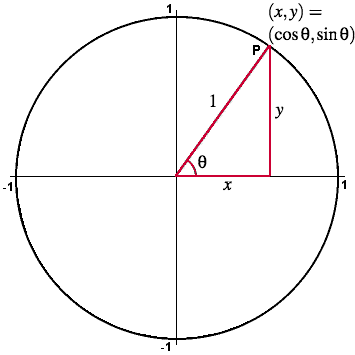
\includegraphics[width=0.5\textwidth]{../figs/unitCircle1.png} % Cambia esta ruta por la ubicación de tu imagen
            \caption{Coordenadas de los puntos sobre una circunferencia unitaria.}
            \label{fig:unitCircle1} % Etiqueta para hacer referencia a la imagen
        \end{figure}
        Por lo tanto, se propone una parametrización de la circunferencia unitaria de la forma:
        \begin{equation*}
            \boldsymbol{\sigma}:[0,2\pi)\rightarrow\mathbb{R}^2/ \\ \boldsymbol{\sigma}(t)=(\cos{t},\sin{t})
        \end{equation*}
        Así, si se graficase $\text{Img}(\boldsymbol{\sigma})$ como puntos en el plano se obtendría toda la circunferencia unitaria.
        Vale aclarar que se tomó el dominio como cerrado en $0$ y abierto en $2\pi$, para que, puesto que ambos valores de 
        entrada corresponden al mismo punto de salida, la parametrización no tenga "puntos repetidos", es decir, que sea inyectiva 
        (análogo a la inyectividad de funciones de $\mathbb{R}$ a $\mathbb{R}$).

        Para contemplar circunferencias de radio distinto de 1, vale con multiplicar el radio a cada componente de la parametrización.
        Además, para parametrizar aquellas que no estén centradas en el orígen, se desplaza cada punto de salida de la
        parametrización por $(x_0,y_0)$, el centro de la nueva circunferencia.
        Por lo tanto, la parametrización de una circunferencia de radio $r\in\mathbb{R}^+$ centrada en $(x_0,y_0)$ es:
        \begin{equation*}
            \boldsymbol{\sigma}:[0,2\pi)\rightarrow\mathbb{R}^2/ \\ \boldsymbol{\sigma}(t)=(r\cdot\cos{t}+x_0,r\cdot\sin{t}+y_0)
        \end{equation*} 
    \end{example}
\end{definition}
        \section{Nociones de Topolog\'ia}
            \begin{definition} [Bola de radio $\delta$ y centro $x_o$] \label{def:bola}
    Sean $x_o \in \Re^n,\;\delta > 0$ y $\text{d}$ una distancia en $\Re^n$. La \emph{bola de radio $\delta$ y centro $x_o$}, que denotamos con $B_{\delta}(x_o)$, es el conjunto:
    \[
     B_{\delta}(x_o) = \left\lbrace x \in \Re^n : \text{d}(x,x_o) < \delta \right\rbrace.
    \]
    El conjunto
    \[
     B^*_{\delta}(x_o) = B_{\delta}(x_o) - \{ x_o \}
    \]
    es la \emph{bola reducida de radio $\delta$ y centro $x_o$}.
   
   \end{definition}
   
   \begin{definition} [Punto interior, interior de un conjunto] \label{def:interior}
    Sean $A \subset \Re^n \text{ y } x_o \in A$. Decimos que $x_o$ es \emph{punto interior} de $A$ si
    \[
     \exists \delta > 0 / B_{\delta}(x_o) \subset A.
    \]
    El \emph{interior} de $A$, que denotamos con $\interior(A)$ o \AA{}, es el conjunto de todos los puntos interiores de $A$:
    \[
     \interior(A) = \left\lbrace x \in A : x \text{ es punto interior de } A \right\rbrace.
    \]
   \end{definition}
   
   \begin{definition} [Conjunto abierto] \label{def:abierto}
       Sea $A \subset \Re^n$. Decimos que $A$ es \emph{abierto} si
   \[
        \forall x_o \in \exists \delta > 0 : B_{\delta}(x_o) \subset A.\footnote{\text{i.e.: $A$  es abierto si todos sus puntos son interiores.}}
   \]
   \end{definition}
   
   \begin{propertie} \label{prop:abierto_int} 
     Un conjunto $A \subset \Re^n$ es abierto si y solo si $A = \interior(A)$.
   \end{propertie}
   
   \begin{definition} [Conjunto cerrado] \label{def:cerrado}
    Sea $A \subset \Re^n$. Decimos que $A$ es \emph{cerrado} si su complemento $A^c = \Re^n - A$ es abierto.
   \end{definition}
   
   \begin{definition} [Frontera de un conjunto] \label{def:frontera}
    Sea $A \subset \Re^n$. La \emph{frontera} de $A$, que denotamos con $\front A$ o $\frontera(A)$, es el conjunto:
    \[
     \front A = \left\lbrace x_o \in \Re^n : \forall \delta > 0 \,
     B_{\delta}(x_o) \cap A \ne \emptyset \wedge
     B_{\delta}(x_o) \cap A^c \ne \emptyset \right\rbrace.
    \]
   \end{definition}
   
   \begin{propertie} \label{prop:cerrado_front}
    Un conjunto $A \subset \Re^n$ es cerrado si y solo si $\front A \subset A$.
   \end{propertie}
   
   \begin{definition} [Punto de acumulaci\'on] \label{def:pto_acum}
    Sean $A \subset \Re^n \text{ y } x_o \in \Re^n$. Decimos que $x_o$ es \emph{punto de acumulaci\'on} de $A$ si
    \[
     \forall \delta > 0 \left( B_{\delta}(x_o) - \{ x_o \} \right) \cap A \ne \emptyset. 
    \]
    Denotamos el conjunto de todos los puntos de acumulaci\'on de $A$ con $A'$:
    \[
     A' = \{ x \in \Re^n : x \text{ es punto de acumulaci\'on de } A \}.
    \]
   
   \end{definition}
   
   \begin{definition} [Entorno de un punto] \label{def:entorno}
    Sean $N \subset  \Re^n$ y $x_o \in \Re^n$. Decimos que $N$ es \emph{entorno} de $x_o$ si
    \[
     \exists \delta > 0 : B_{\delta}(x_o) \subset N.
    \]
   \end{definition}
   
   \begin{definition} [Punto aislado] \label{def:pto_ais}
    Sean $A \subset  \Re^n$ y $x_o \in A$. Decimos que $x_o$ es \emph{punto aislado} de $A$ si $x_o$ no es punto de acumulaci\'on de $A$.
   \end{definition}
   
   \begin{definition} [Conjunto acotado] \label{def:conj_acotado}
    Sea $A \subset \Re^n$. Decimos que $A$ es un \emph{conjunto acotado} si existe $\delta > 0$ tal que la bola de radio $\delta$  centrada en el origen contiene al conjunto $A$, es decir, si $\exists \delta > 0 : A \subset B_{\delta}(\mathbf{0})$.\\
    Equivalentemente, $A$ es un \emph{conjunto acotado} si $\exists \delta > 0, x_o \in \Re^n : A \subset B_{\delta}(x_o)$.
   \end{definition}
   
        \section{Gráfica}
            
Observacion: \textcolor{red}{(enumerar)} Si en la definic\'ion \textcolor{red}{(recuerdo de mate 1. poner referencia)} (\ref{grafm1}) cambiemos  $A \subseteq \mathbb{R}$ por $A \subseteq \mathbb{R}^{n}$  obtenemos de manera an\'aloga la siguiente definici\'on.    




\begin{definition}  \label{def:grafica}
 
 Sea $f: A\subseteq\Rn{n}\rightarrow\R$; se define la \textit{gráfica de $f$ }, y se nota $graf(f)$,  a
 \[
graf(f)=\{(x_1,x_2,...,x_n,x_{n+1})\in \mathbb{R}^{n+1} \backslash (x_1,x_2,...,x_n) \in A \land f(x_1,x_2,...,x_n)=x_{n+1} \}
 \]


Observaci\'on: \textcolor{red}{Enumerar}   Si $f: A\subseteq\Rn{n}\rightarrow\R$ entonces $graf(f) \subset \mathbb{R}^{n+1}.$
 

Observaci\'on: \textcolor{red}{Enumerar} Dada la  anterio observaci\'onr y con el objetivo de poder dibujar,  nos detendremos especialmente en el caso de gr\'aficas de  campos  $f: A\subseteq\Rn{2}\rightarrow\R,$ cuya definici\'on se desprende automaticamente  de  (\ref{def:grafica}), o sea, el caso
 \[
graf(f)=\{(x,y,z)\in\Rn{3} \backslash (x,y)\subseteq A \land z=f(x,y) \}
 \]



\textcolor{red}{Todo esto va en el recuerdo de mate 1 para completar y corregir los ejemplos------------------------}
\begin{figure}[h!] % El entorno figure te permite incluir imágenes
    \centering
    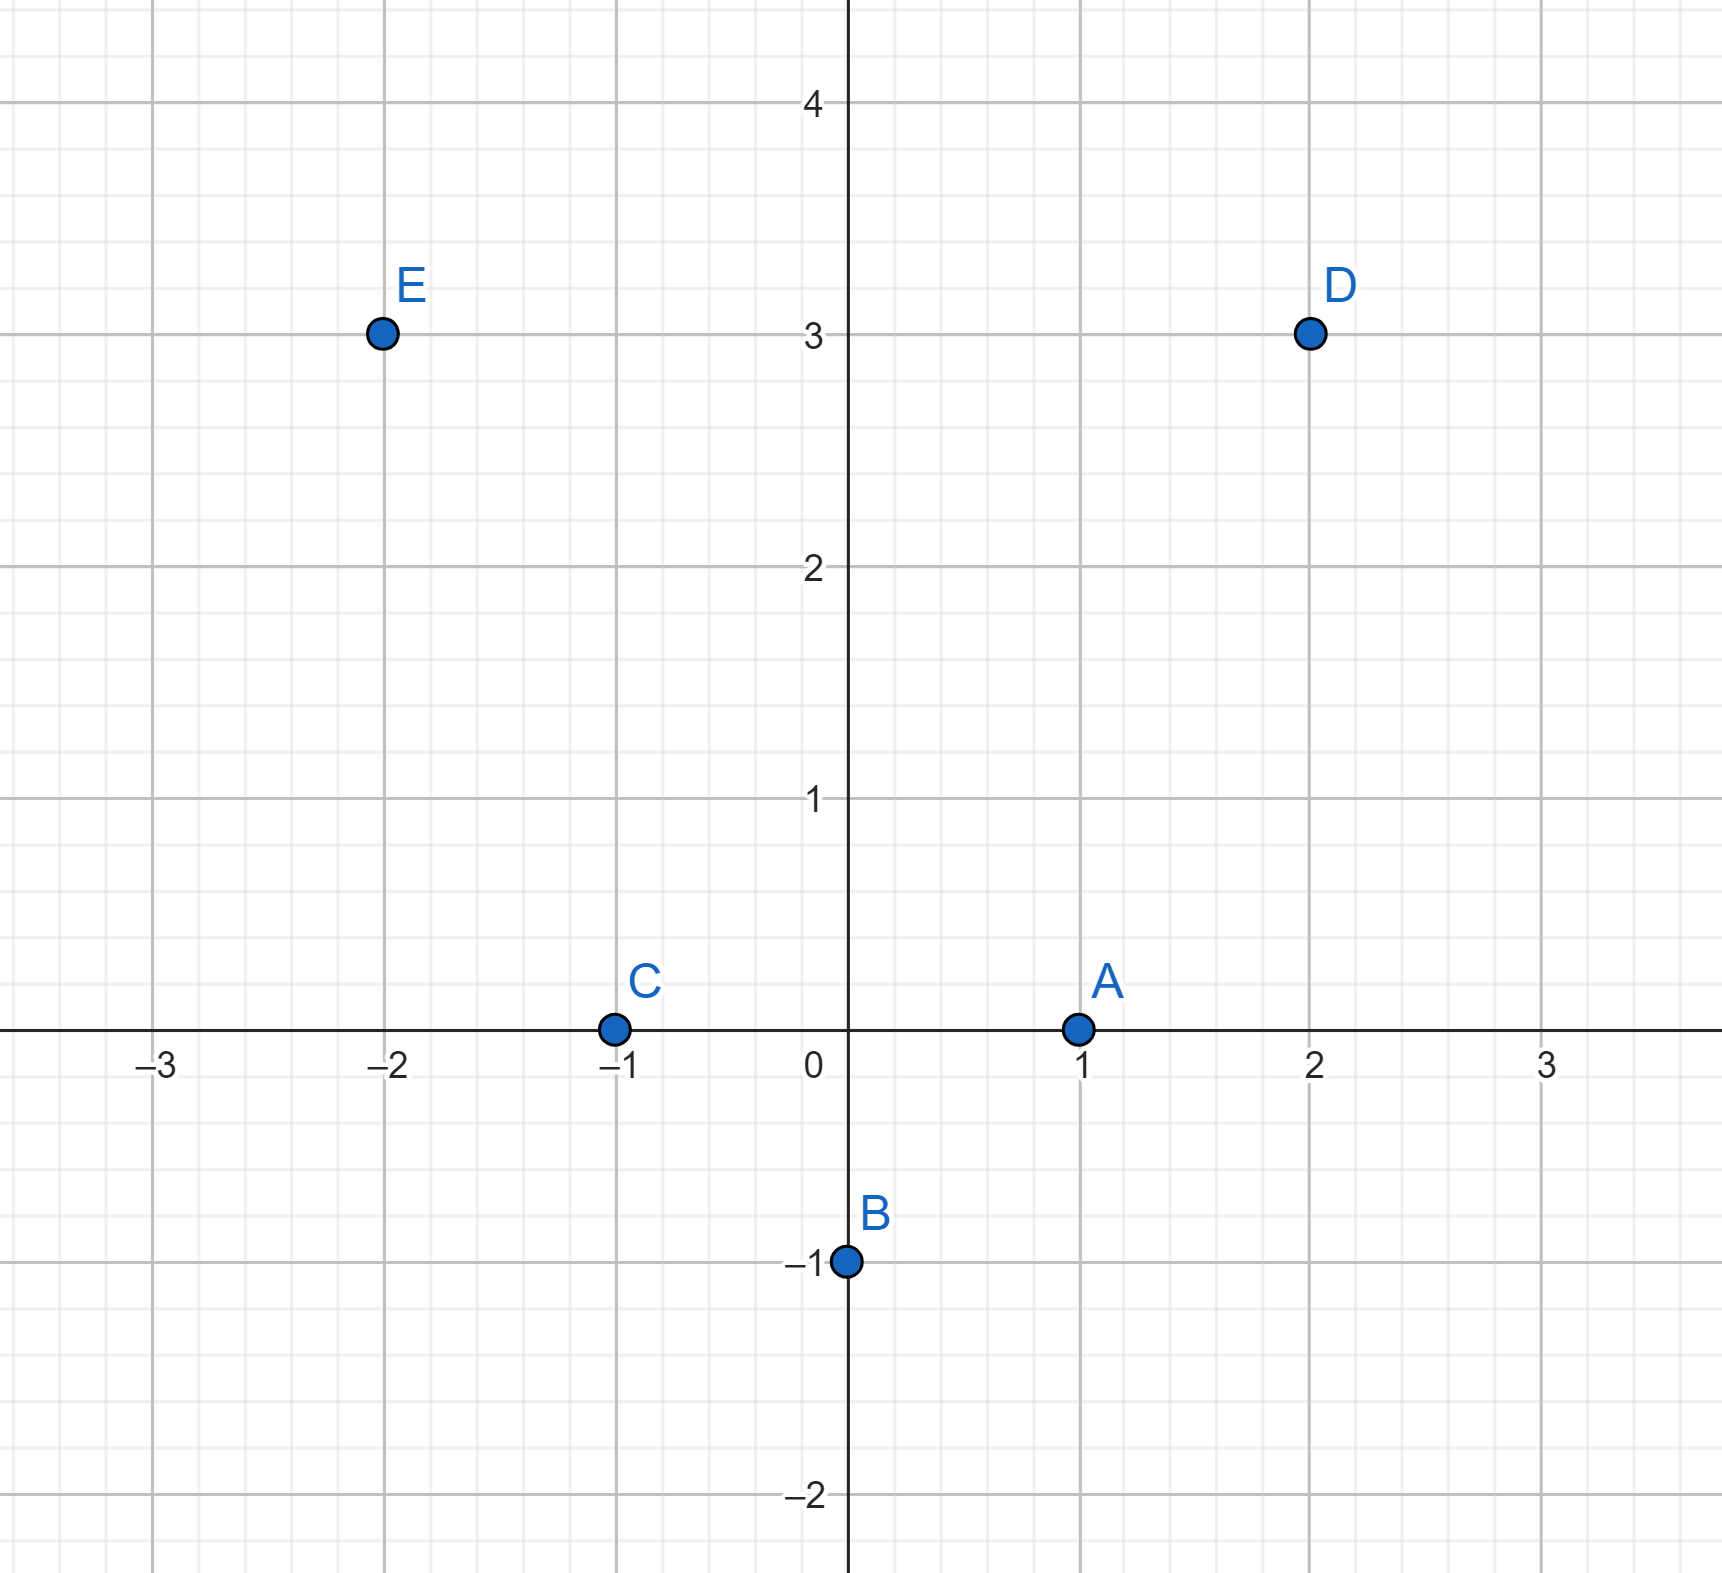
\includegraphics[width=0.34\textwidth]{../figs/Puntos_grafica.png} % Cambia esta ruta por la ubicación de tu imagen
    \caption{Puntos de tabla 1.}
    \label{fig:ejemplo1} % Etiqueta para hacer referencia a la imagen
\end{figure}


De esta manera, se puede empezar a representar la grafica de $f$
\begin{figure}[h!] % El entorno figure te permite incluir imágenes
    \centering
    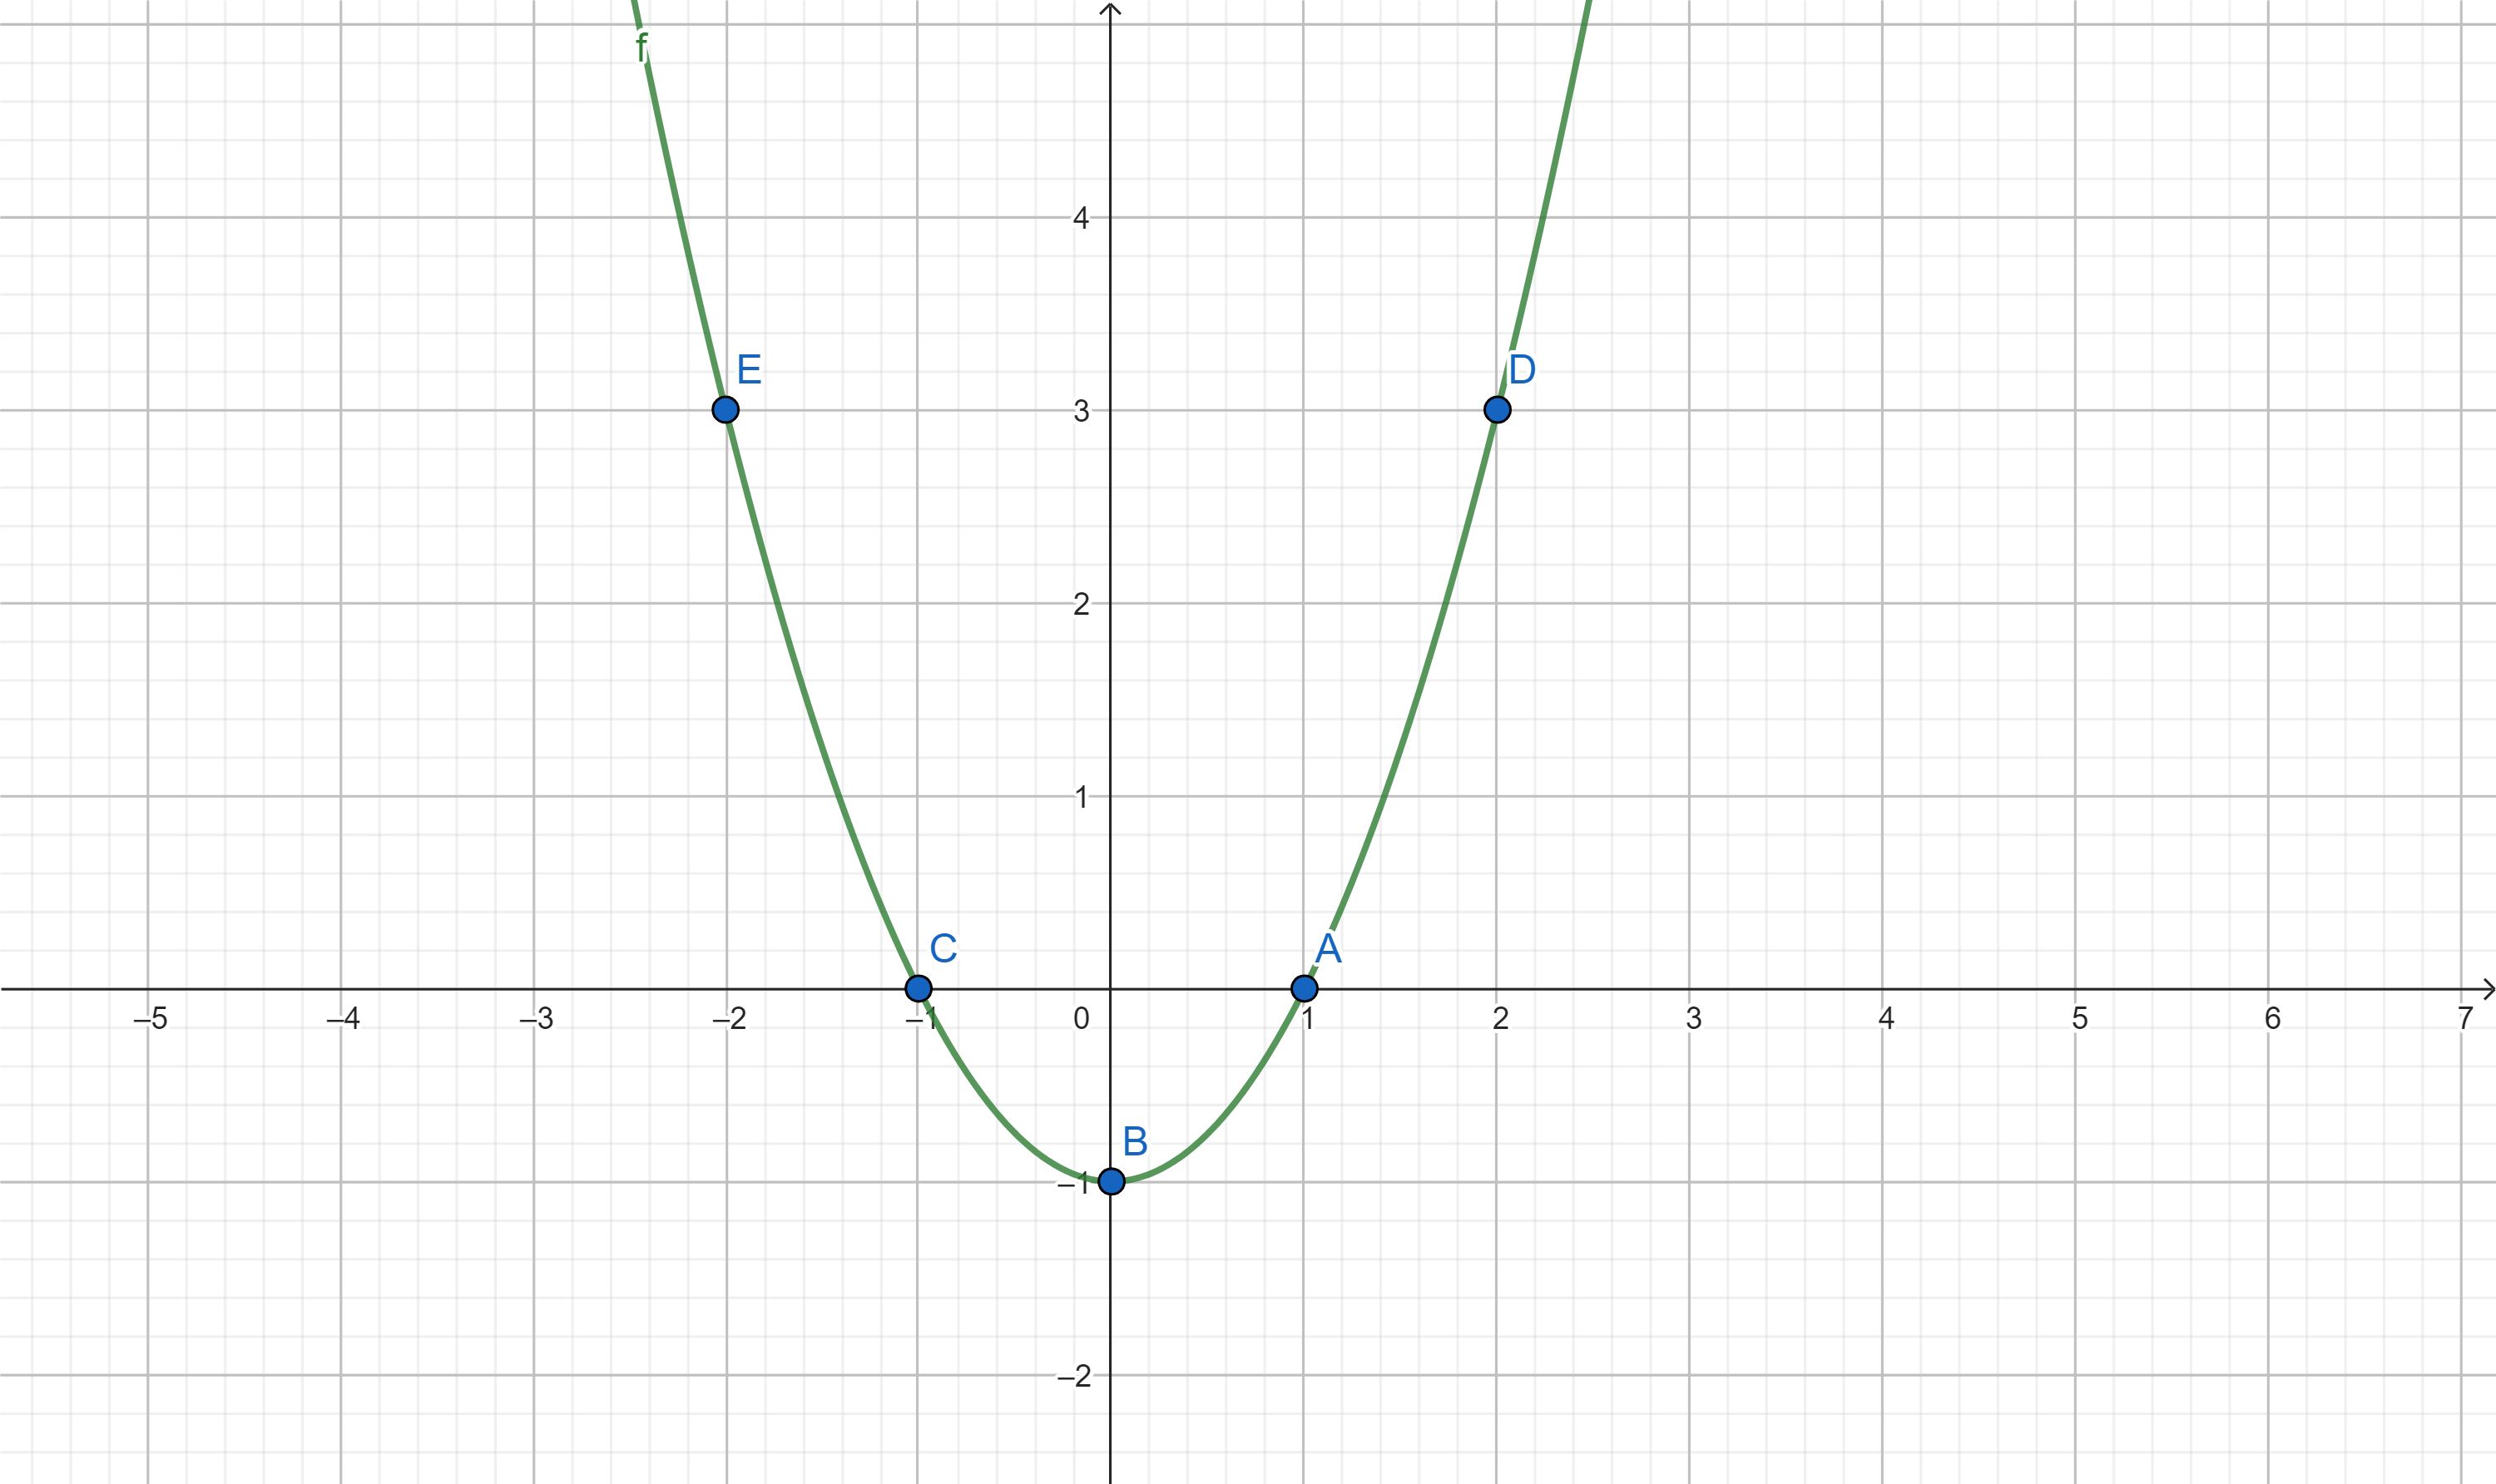
\includegraphics[width=0.5\textwidth]{../figs/r2_grafica.png} % Cambia esta ruta por la ubicación de tu imagen
    \caption{Grafica de $f(x)$.}
    \label{fig:ejemplo2} % Etiqueta para hacer referencia a la imagen
\end{figure}
\end{definition}
\textcolor{red}{Hasta aca---------------------------------------------------------------------------------------------------------}

\vspace{1 cm}

\textcolor{red}{no esta definido conjuntos de nivel --------------------------------------------------------------------------}


En este curso, se analizaran las graficas de funciones en  $\Rn{3}$. Analizamos un ejemplo, tomando $h(x,y)=x^2+y^2$.
Para la función , que representa un paraboloide, los conjuntos de nivel están dados por $h(x,y)=c$, que son círculos concéntricos en el plano xy. Graficando esta función en 3D, podemos ver una superficie parabólica, donde los conjuntos de nivel son las proyecciones de estas circunferencias a diferentes alturas en el eje z y con radio creciente.
\begin{figure}[h!] % El entorno figure te permite incluir imágenes
    \centering
    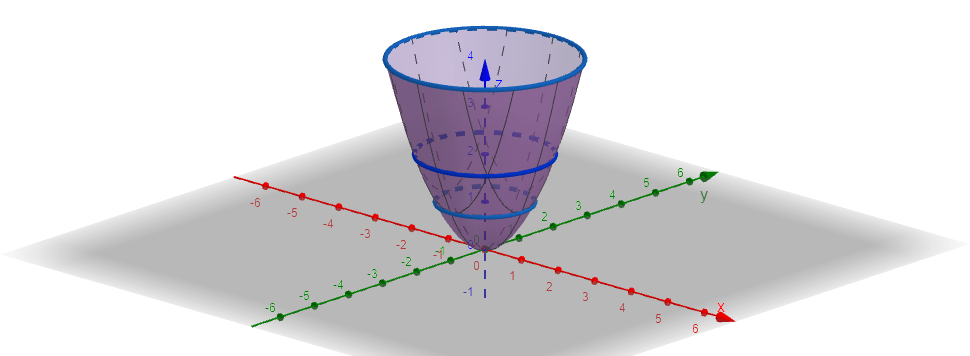
\includegraphics[width=1\textwidth]{../figs/r3_grafica.png} % Cambia esta ruta por la ubicación de tu imagen
    \caption{\small{ Gráfica de h y conjuntos de nivel tomando 
    c=\{1,2,4}\}}
    \label{fig:ejemplo3} % Etiqueta para hacer referencia a la imagen
\end{figure}


\textcolor{red}{Hasta aca---------------------------------------------------------------------------------------------------------}

        \section{Conjunto de nivel}
            
\begin{definition} [Conjunto de nivel] 
\label{def:conjunto de nivel}
 \mbox{}
 
Sea $f: U\subset\Rn{n}\rightarrow\R$ y sea $c \in \R$, se define  el conjunto de nivel de $f$ de nivel  $c$, y se nota $C(c,f)$,  a  
\[
C(c,f)=\{ x \in U \backslash f (x)=c \}.
 \]





Es decir,  $C(c,f)$ son aquellos puntos $x\in\ U$ para las cuales $f(x)=c$, o dicho de otra manera,  $C(c,f)$ es la preimagen de $c$ por $f$.   Si $n=2$ hablamos de curva de nivel  y si $n=3$  hablamos de superficie de nivel  

Observaci\'on: \textcolor{red}{Enumerar}   Si $f: A\subseteq\Rn{n}\rightarrow\R$ entonces $C(c,f)  \subset \mathbb{R}^{n}.$



\begin{example}   Sea  el campo  $f: \mathbb{R}^{2} \rightarrow \mathbb{R} \:|\:  f(x,y)=x^2+y^2.$
\end{example}
1. Calcular y graficar los conjuntos de nivel de $f$.

2. Hacer un gr\'afico de  $graf(f)$.



Observemos que, dado $c \in \mathbb{R}$: 
 $$C(c,f)=\{(x,y) \in U \backslash   x^2+y^2  =c \}.$$
 Tomando, para ilustrar,  $c=0$, $c=1$ y $c=4$, quedando (ver (\ref{circ})) 
 \[
C(0,f)=\{(x,y) \in U \backslash x^2+y^2=0 \}
\]
 \[
C(1,f)=\{(x,y) \in U \backslash x^2+y^2=1 \}
\]
 \[
C(4,f)=\{(x,y) \in U \backslash x^2+y^2=4 \}
 \]

\begin{figure}[h!] % El entorno figure te permite incluir imágenes
    \centering
    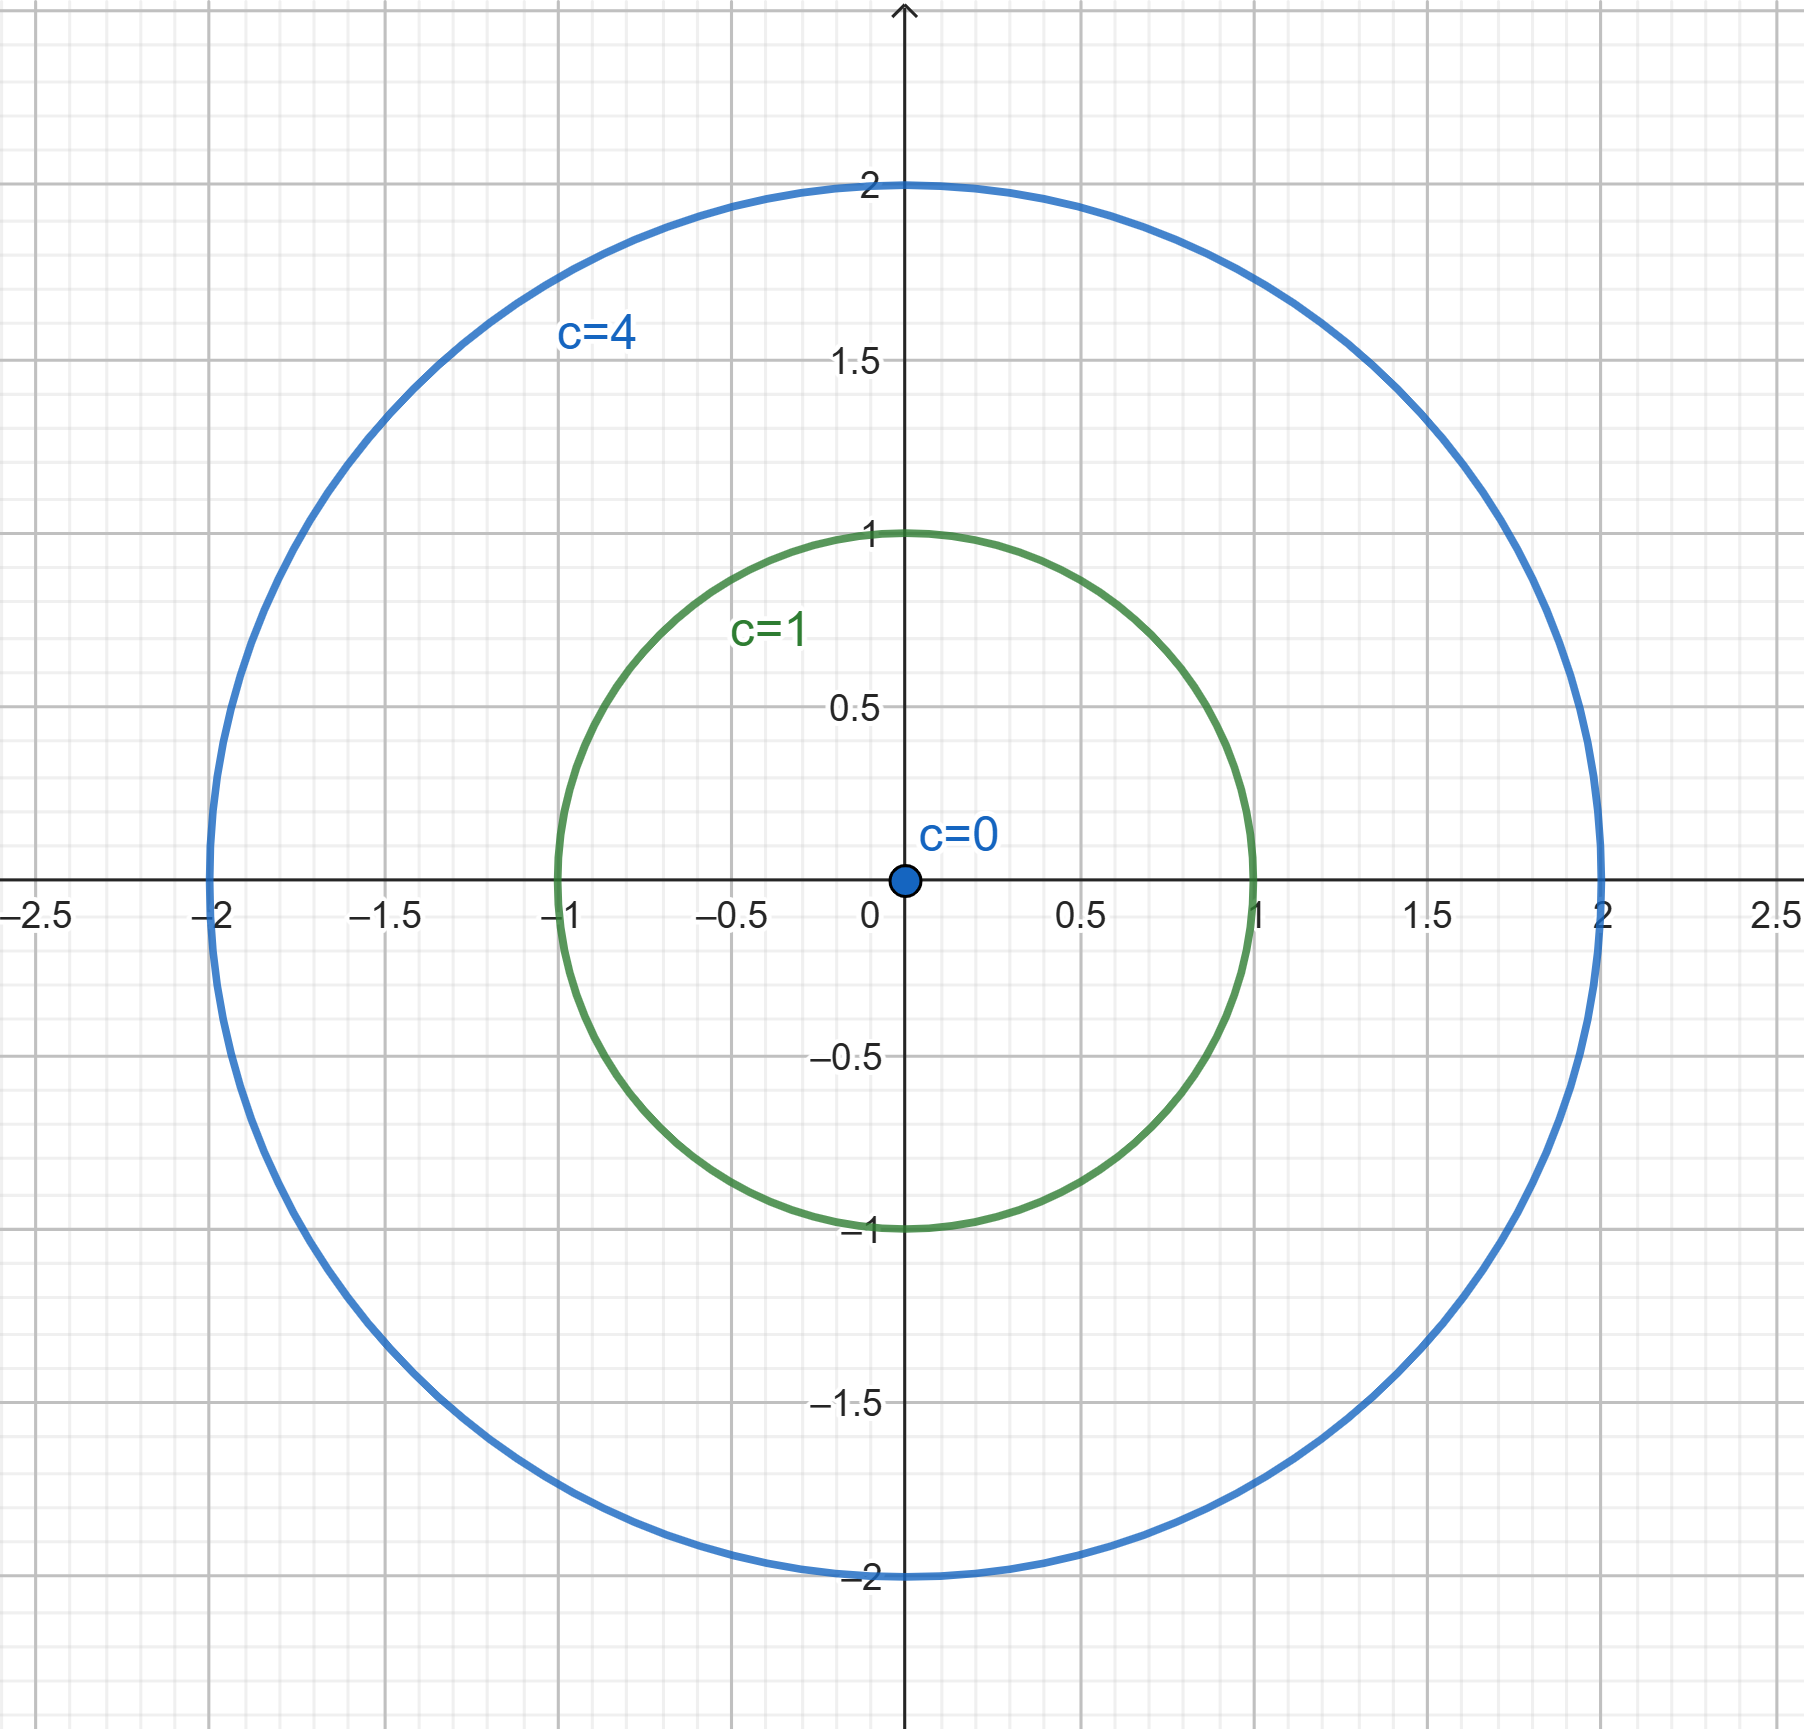
\includegraphics[width=0.5\textwidth]{../figs/conjunto1_r.png} % Cambia esta ruta por la ubicación de tu imagen
    \caption{Conjuntos de nivel}
    \label{fig:ejemplo} % Etiqueta para hacer referencia a la imagen
\end{figure}

En general, podemos determinar: 

   \[
        C(c,f)=
        \begin{dcases}
           \textnormal{Circunferencia centrada en (0,0) de radio} \sqrt{c},  & \textnormal{si}:  c>0 \\
(0,0)  & \textnormal{si}:\ c=0\\
\emptyset  & \textnormal{si}:\ c<0\\
        \end{dcases}
    \]

\textcolor{red}{Aca ``dibujar'' los conjuntos de nivel en $\mathbb{R}^{3}$ y notar que no es suficinte para graficar.}  


\textcolor{red}{Definir cortes transversales y dibujarlos.}


\begin{figure}[h!] % El entorno figure te permite incluir imágenes
    \centering
    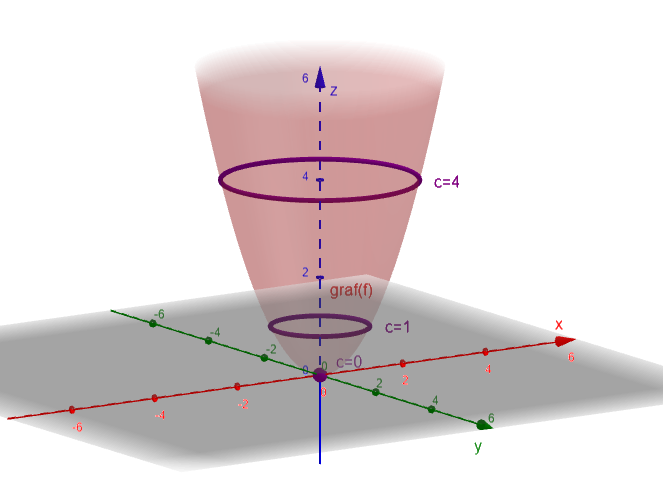
\includegraphics[width=0.5\textwidth]{../figs/conjunto1_r3.png} % Cambia esta ruta por la ubicación de tu imagen
    \caption{graf(f)}
    \label{fig:ejemplo} % Etiqueta para hacer referencia a la imagen
\end{figure}



 

\begin{example}   Sea  el campo  $g: \mathbb{R}^{2} \rightarrow \mathbb{R} \:|\:  g(x,y) = \sqrt{x^2+y^2}.$
\end{example}
1. Calcular y graficar los conjuntos de nivel de $g$.

2. Hacer un gr\'afico de  $graf(g)$.


\textcolor{red}{Resolver identico al ejercicio  anterior.}  



: Se toma la funcion $f(x,y)=\sqrt{x^2+y^2}$, donde empezamos a analizar los distintos conjuntos de nivel, tomando $c$ con diferentes constantes
 \[
C(0,f)=\{(x,y) \in U \backslash \sqrt{x^2+y^2}=0 \}
\]
 \[
C(1,f)=\{(x,y) \in U \backslash \sqrt{x^2+y^2}=1 \}
\]
 \[
C(2,f)=\{(x,y) \in U \backslash \sqrt{x^2+y^2}=2 \}
 \]

\begin{figure}[h!] % El entorno figure te permite incluir imágenes
    \centering
    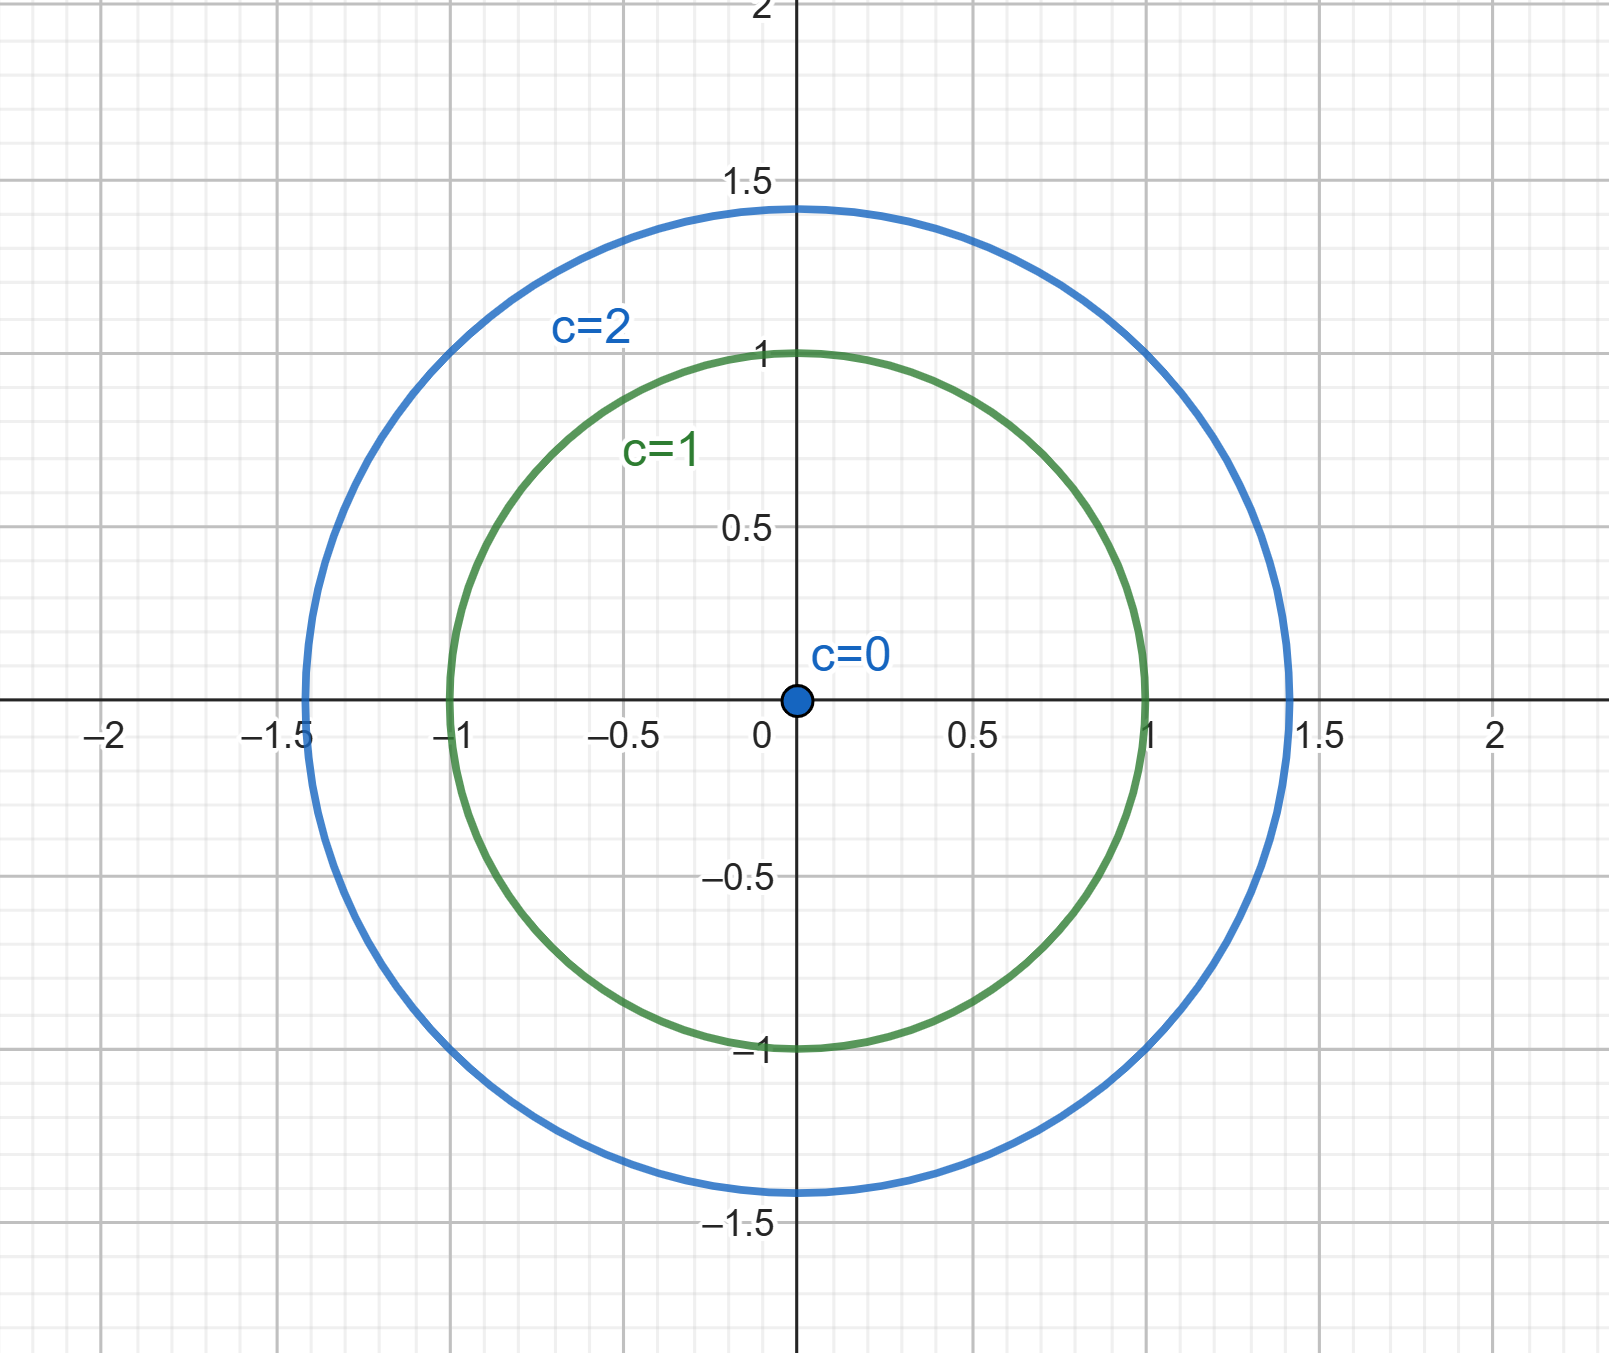
\includegraphics[width=0.5\textwidth]{../figs/conjunto2_r2.png} % Cambia esta ruta por la ubicación de tu imagen
    \caption{Conjuntos de nivel}
    \label{fig:ejemplo} % Etiqueta para hacer referencia a la imagen
\end{figure}

En general, podemos determinar: 

   \[
        C(c,f)=
        \begin{dcases}
           \textnormal{Circunferencia centrada en (0,0) de radio} c,  & \textnormal{si}:  c>0 \\
(0,0)  & \textnormal{si}:\ c=0\\
\emptyset  & \textnormal{si}:\ c<0\\
        \end{dcases}
    \]
\begin{figure}[h!] % El entorno figure te permite incluir imágenes
    \centering
    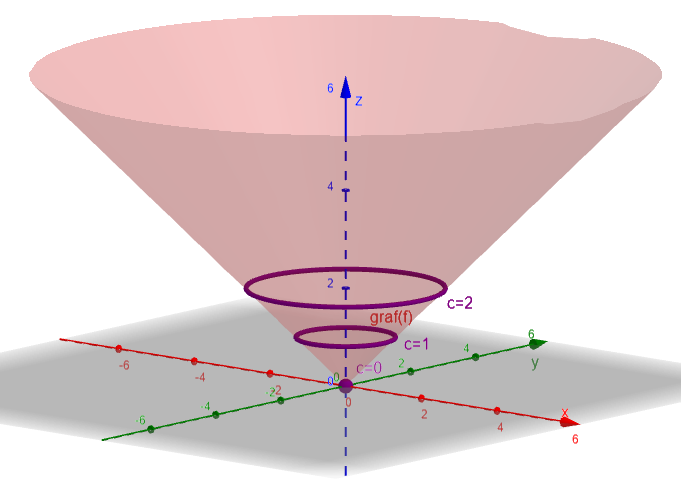
\includegraphics[width=0.5\textwidth]{../figs/conjunto2_r3.png} % Cambia esta ruta por la ubicación de tu imagen
    \caption{Conjuntos de nivel y graf(f)}
    \label{fig:ejemplo} % Etiqueta para hacer referencia a la imagen
\end{figure}

De esta manera, considerando la definicion de gráfica de una funci\'on, podemos representar la misma en $\Rn{3}$ tomando  la ecuaci\'on de la parte superior de un cono: $z=\sqrt{x^2+y^2}$



\textcolor{red}{Corregir esta observaci\'on. esta mal escrito, quien es la funci\'on f?}


Observaci\'on \textcolor{red}{enumerar}:Dada la  ecuaci\'on $z^2=x^2+y^2$ al despejar z obtenemos $|z|=\sqrt{x^2+y^2}$ obtendriamos que: 
 \[
        C(c,f)=
        \begin{dcases}
           \textnormal{Circunferencia centrada en (0,0) de radio} c,  & \textnormal{si}:  c>0 \\
(0,0)  & \textnormal{si}:\ c=0\\
\textnormal{Circunferencia centrada en (0,0) de radio} c,  & \textnormal{si}:\ c<0\\
        \end{dcases}
    \]

De esta manera, considerando la definicion de gráfica de una funcion, podemos representar la misma en $\Rn{3}$ tomando  la ecuacion del cono: $z^2=x^2+y^2$

\begin{figure}[h!] % El entorno figure te permite incluir imágenes
    \centering
    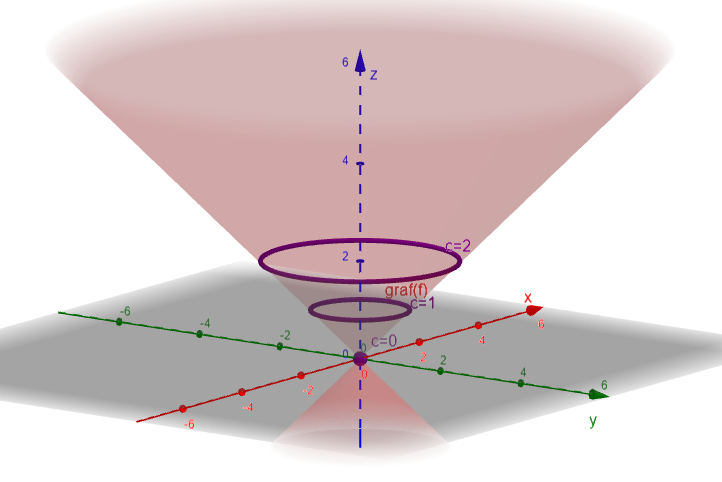
\includegraphics[width=0.5\textwidth]{../figs/conjunto3_r3.png} % Cambia esta ruta por la ubicación de tu imagen
    \caption{Conjuntos de nivel y graf(f)}
    \label{fig:ejemplo} % Etiqueta para hacer referencia a la imagen
\end{figure}


\textcolor{red}{Mejorar la figura, no se llega a apreciar el cono completo}

\end{definition}

        \section{L\'imite de Funciones}
            \label{sec:limites}
\begin{definition} [L\'imite] \label{def:limite}
Sean $f:A \subset \Rn{n} \to \Rn{m}$ una funci\'on, $L \in \Rn{m}$ y $x_0$ un punto de acumulaci\'on de $A$. Decimos que \emph{el l\'imite de $f$ para $x$ tendiendo a $x_o$ es $L$} o que \emph{$f$ tiende a $L$ cuando $x$ tiende a $x_o$}
si
\[
 \forall \varepsilon > 0 \, \exists \delta > 0 / f(x) \in B_{\varepsilon}(L) \, \forall 
 x \in B_{\delta}^*(x_o) \cap A.
\]

En este caso, utilizamos la notaci\'on
\[
 f(x) \xrightarrow[x \to x_o]{} L \quad \text{o} \quad \lim_{x \to x_o} f(x) = L.
\]
\begin{obs} Si $f$ es un \emph{campo escalar} (es decir, si en la definici\'on \eqref{def:limite} es $m = 1$), la condici\'on 
 \[
 \forall \varepsilon > 0 \, \exists \delta > 0 / f(x) \in B_{\varepsilon}(L) \, \forall 
 x \in B_{\delta}^*(x_o) \cap A
\]
es equivalente a 
\[
 \forall \varepsilon > 0 \, \exists \delta > 0 / \abs{ f(x) - L } < \varepsilon \, \forall 
 x \in B_{\delta}^*(x_o) \cap A.
\]
\end{obs}

\begin{obs} La definici\'on de l\'imite puede expresarse equivalentemente en t\'erminos de distancias o de normas:
\begin{itemize} 
 \item Sean $f:A \subset \Rn{n} \to \Rn{m}$ una funci\'on, $L \in \Rn{m}$ y $x_0$ un punto de acumulaci\'on de $A$. Decimos que \emph{el l\'imite de $f$ para $x$ tendiendo a $x_o$ es $L$} o que \emph{$f$ tiende a $L$ cuando $x$ tiende a $x_o$} si
\[
 \forall \varepsilon > 0 \, \exists \delta > 0 / \dis_m {(f(x),L)} < \varepsilon \, \forall 
 x\in A : 0 < \dis_n {(x,x_o)} < \delta,
\] 
donde $\dis_n$ y $\dis_m$ son las distancias en $\Rn{n}$ y $\Rn{m}$, respectivamente.

 \item Sean $f:A \subset \Rn{n} \to \Rn{m}$ una funci\'on, $L \in \Rn{m}$ y $x_0$ un punto de acumulaci\'on de $A$. Decimos que \emph{el l\'imite de $f$ para $x$ tendiendo a $x_o$ es $L$} o que \emph{$f$ tiende a $L$ cuando $x$ tiende a $x_o$} si
\[
 \forall \varepsilon > 0 \, \exists \delta > 0 / \norm{f(x) - L}_m < \varepsilon \, \forall 
 x\in A : 0 < \norm{x - x_o}_n < \delta,
\] 
donde $\norm{\cdot}_n$ y $\norm{\cdot}_m$ son las normas en $\Rn{n}$ y $\Rn{m}$, respectivamente.
\end{itemize}
\end{obs}

\end{definition}

\begin{theorem}[Unicidad del l\'imite] \label{teo:unicidad_limite}
\mbox{}

Sean $f:A \subset \Rn{n} \to \Rn{m}$ una funci\'on, $x_0$ un punto de acumulaci\'on de $A$ y $L_1, L_2 \in \Rn{m}$ tales que 
\[
 f(x) \xrightarrow[x \to x_o]{} L_1 \quad \wedge \quad f(x) \xrightarrow[x \to x_o]{} L_2.
\]
Entonces $L_1 = L_2$.
\begin{proof}
\mbox{}

Las ideas utilizadas en la demostraci\'on de este teorema son las que siguen.\\
Como 
\[
 f(x) \xrightarrow[x \to x_o]{} L_1,
\]
dado $\varepsilon > 0$ existe alg\'on $\delta_1 > 0$ tal que cada punto $x \in B_{\delta_1}^*(x_o) \cap A$ se aplica a trav\'es de $f$ en alg\'on punto de la bola de centro $L_1$ y radio $\varepsilon$.

\def\Ro{2.0}
\def\Rb{1.0}
\def\Ra{3.0}
\def\sep{1.0*\Ro}

\input{../figs/fig1}


De la misma manera, como 
\[
 f(x) \xrightarrow[x \to x_o]{} L_2,
\]
dado $\varepsilon > 0$ existe alg\'on $\delta_2 > 0$ tal que cada punto $x \in B_{\delta_2}^*(x_o) \cap A$ se aplica a trav\'es de $f$ en alg\'on punto de la bola de centro $L_2$ y radio $\varepsilon$.

\input{../figs/fig2}

Si suponemos que $L_1 \ne L_2$, por propiedad de la distancia es $\dis(L_1,L_2) > 0$ y podemos elegir 
\[
 \varepsilon = \frac{\dis{(L_1,L_2)}}{2}.
\]
Para este valor de $\varepsilon$ podemos encontrar un punto $x$ que se aplica por $f$ en alg\'on punto de la bola de centro $L_1$ y radio $\varepsilon$ \textbf{y tambi\'en} se aplica por $f$ en alg\'on punto de la bola de centro $L_2$ y radio $\varepsilon$, lo cual es absurdo, pues estas dos bolas son disjuntas.

\input{../figs/fig3}

Ahora s\'i, veamos la demostraci\'on formal del teorema.\\
 Supongamos, por el absurdo, que $L_1 \ne L_2$, y sea $\varepsilon = \dis(L_1,L_2)/2 > 0.$ \\ 
 Como 
 \[
  f(x) \xrightarrow[x \to x_o]{} L_1,
 \]
podemos elegir $\delta_1 > 0$ tal que $x \in B_{\delta_1}^*(x_o) \cap A \then f(x) \in B_{\varepsilon}(L_1)$.\\
Como 
\[
 f(x) \xrightarrow[x \to x_o]{} L_2,
\]
 podemos elegir $\delta_2 > 0$ tal que $x \in B_{\delta_2}^*(x_o) \cap A \then f(x) \in B_{\varepsilon}(L_2)$.\\
 Notemos que, como sugiere la figura, 
 \[
  B_{\varepsilon}(L_1) \cap B_{\varepsilon}(L_2) = \emptyset.
 \]
 En efecto, de no ser as\'i, sea $z \in B_{\varepsilon}(L_1) \cap B_{\varepsilon}(L_2)$. Tenemos que:
 \[
  2 \varepsilon = \dis(L_1,L_2) \le \dis(L_1,z) + \dis(z,L_2)
  < \varepsilon + \varepsilon = 2 \varepsilon \then \varepsilon < \varepsilon. \text{ Absurdo.}
 \]

 Sea $\delta = \min\{ \delta_1, \delta_2 \}$. \\
 Como $B_{\delta}^*(x_o) \subset B_{\delta_1}^*(x_o)$ y $B_{\delta}^*(x_o) \subset B_{\delta_2}^*(x_o)$, si tomamos alg\'on $x \in B_{\delta}^*(x_o) \cap A$\footnote{Notemos que $B_{\delta}^*(x_o) \cap A \ne \emptyset$ porque $x_o$ es un punto de acumulaci\'on de $A$.}, vale que $f(x) \in B_{\varepsilon}(L_1)$ y tambi\'en $f(x) \in B_{\varepsilon}(L_2)$, por lo que $f(x) \in B_{\varepsilon}(L_1) \cap B_{\varepsilon}(L_2)$. Absurdo, pues $B_{\varepsilon}(L_1) \cap B_{\varepsilon}(L_2) = \emptyset$. El absurdo provino de suponer que $L_1 \ne L_2$, por lo cual debe ser $L_1 = L_2$.

\end{proof}

\end{theorem}
\begin{propertie}[\'algebra de l\'imites] \label{prop:alg_lim} Sean $f,g:A \subset \Rn{n} \to \Rn{m}$ funciones y $x_0$ un punto de acumulaci\'on de $A$. Supongamos que 
  \begin{align*}
   &\lim_{x \to x_o} f(x) = L_1 \in \Rn{m} \\
   &\lim_{x \to x_o} g(x) = L_2 \in \Rn{m}.
  \end{align*}
  Entonces:
  \begin{enumerate} %[i.]
   \item Linealidad
      \begin{enumerate} %[(a)]
       \item $\lim_{x \to x_o} (f + g)(x) = L_1 + L_2$
       \item $\lim_{x \to x_o} (\alpha f)(x) = \alpha L_1 \, \forall \alpha \in \R$
      \end{enumerate}
  \item $\lim_{x \to x_o} (f \cdot g) (x) = L_1 \cdot L_2$\footnote{Si $m \ge 2$, ``$\cdot$'' representa el producto escalar en $\Rn{m}$.}
  \item Si $m = 1$ (i.e., si $f \text{ y } g$ son campos escalares), $g$ es no nula en alg\'on entorno de $x_o$ y $L_2 \ne 0$, 
  \[
   \lim_{x \to x_o} \frac{f(x)}{g(x)} = \frac{L_1}{L_2}.
  \]
  \end{enumerate}
\end{propertie}

\begin{propertie} \label{prop:lim_x_comp}
 Sea $F: A \subset \Rn{n} \to \Rn{m}$ un campo vectorial y $x_0$ un punto de acumulaci\'on de $A$. Sean $f_j: A \subset \Rn{n} \to \R \, (j = 1,2, \dots, m)$ campos escalares tales que $F(x) = \left( f_1(x), f_2(x), \dots, f_m(x) \right) \, \forall x \in A$\footnote{Los campos escalares $f_j$ quedan determinados un\'ivocamente por $F$ de la siguiente manera: 
 \begin{align*}
     f_j &: A \subset \Rn{n} \to \R \\
     &f_j(x) = F(x) \cdot e_j,
 \end{align*} donde $e_j$ es el $j$-\'esimo vector can\'onico de $\Rn{m}$.}.\\
 Sea $L = \left( L_1, L_2, \dots, L_m \right) \in \Rn{m}$, $L_j \in \R \, \forall j = 1,2, \dots, m$. Entonces:
 \[
  \lim_{x \to x_o} F(x) = L \iff \lim_{x \to x_o} f_j(x) = L_j \, \forall j = 1,2, \dots, m.
 \]

\end{propertie}


  \begin{propertie} \label{prop:lim_1}
    Sean $f:A \subset \Rn{n} \to \R$ una funci\'on y $x_0$ un punto de acumulaci\'on de $A$. Las siguientes proposiciones son equivalentes:
 \begin{enumerate} %[i.]
  \item $\lim_{x \to x_o} f(x) = 0$.
  \item $\lim_{x \to x_o} | f(x) | = 0$.
 \end{enumerate}
 \begin{proof}
 \mbox{}
 
 \begin{enumerate} %[(a)]
  \item Veamos que (I) implica (II). Como 
  \[
   \lim_{x \to x_o} f(x) = 0,
  \]
  por definici\'on de l\'imite, dado $\varepsilon > 0$ podemos tomar $\delta > 0$ tal que 
  \[
   \abs{f(x) - 0} < \varepsilon \, \forall x \in B^*_{\delta}(x_o) \cap A.
  \]
  Para este valor de $\delta$ se cumple que
  \[
   \Big| \abs{f(x)} - 0 \Big| = \Big| \abs{f(x)} \Big| = \abs{f(x)} = \abs{f(x) - 0} < \varepsilon \, 
   \forall x \in B^*_{\delta}(x_o) \cap A,
  \]
  de modo que, por definici\'on, 
  \[
   \lim_{x \to x_o} \abs{ f(x) } = 0.
  \]
  \item Veamos que (II) implica (I). Como
  \[
   \lim_{x \to x_o} \abs{ f(x) } = 0,
  \]
  por definici\'on de l\'imite, dado $\varepsilon > 0$ podemos tomar $\delta > 0$ tal que 
  \[
   \Big| \abs{f(x)} - 0 \Big| < \varepsilon \, \forall x \in B^*_{\delta}(x_o) \cap A.
  \]
  Para este valor de $\delta$ se cumple que
  \[
   \abs{f(x) - 0} = \abs{f(x)} = \Big| \abs{f(x)} \Big| = \Big| \abs{f(x)} - 0 \Big| < \varepsilon \, 
   \forall x \in B^*_{\delta}(x_o) \cap A,
  \]
  de modo que, por definici\'on, 
  \[
   \lim_{x \to x_o} f(x) = 0.
  \]
 \end{enumerate}

  
 \end{proof}

\end{propertie} 

\begin{propertie} \label{prop:sandwich} %[Principio de intercalaci\'on]
Sean $f, g, h : A \subset \Rn{n} \to \R$ funciones y $x_0$ un punto de acumulaci\'on de $A$. Supongamos que $\exists \delta_o > 0$ tal que 
\[
 f(x) \le g(x) \le h(x) \, \forall x \in B_{\delta_o}(x_o) \cap A.
\]
Si $\lim_{x \to x_o}f(x) = \lim_{x \to x_o}h(x) = L$, entonces
\[
 \lim_{x \to x_o}g(x) = L.
\]
 
\end{propertie}

\begin{propertie} \label{prop:cero_x_acotada}
 Sean $f, g : A \subset \Rn{n} \to \R$ funciones y $x_0$ un punto de acumulaci\'on de $A$. Si $\exists \delta_o > 0$ tal que $f$ es acotada en $B_{\delta_o}(x_o) \cap A$ (i.e.: $\exists M > 0 \text{ tal que } \abs{f(x)} \le M \forall x \in  B_{\delta_o}(x_o) \cap A$) y $\lim_{x \to x_o}g(x) = 0$, entonces
\[
 \lim_{x \to x_o}(f \cdot g)_{(x)} = 0.
\]
\begin{proof}
\mbox{}

Supongamos que, para cierto $\delta_o > 0$, $f$ es acotada en $B_{\delta_o}(x_o) \cap A$, y sea $M > 0 \text{ tal que } \abs{f(x)} \le M \quad \forall x \in  B_{\delta_o}(x_o) \cap A$.
Como 
\[
\lim_{x \to x_o}g(x) = 0, 
\]
dado $\varepsilon > 0 $, por definici\'on de l\'imite, podemos elegir $\delta_1 > 0$ tal que 
\[
 \abs{g(x)} < \frac{\varepsilon}{M} \quad \forall x \in  B^*_{\delta_1}(x_o) \cap A.                                                                                               
\]
Sea $\delta = \min{ \left\{ \delta_o, \delta_1 \right\} }$. \\
Se cumple que
\[
 \abs{ (f \cdot g)_{(x)} - 0 } = \abs{ f(x) \cdot g(x) } = \abs{f(x)}\abs{g(x)} \le 
 M \abs{g(x)} < M \frac{\varepsilon}{M} = \varepsilon \quad \forall x \in  B^*_{\delta}(x_o) \cap A,
\]
Por lo tanto, por definici\'on de l\'imite,
\[
 \lim_{x \to x_o}(f \cdot g)_{(x)} = 0.
\]

\end{proof}
\end{propertie}


\begin{propertie} [L\'imite de la composici\'on] \label{prop:lim_comp}
\mbox{}

Sean $f, g$ funciones 
\begin{align*}
 g &:A \subset \Rn{n} \to B \subset \Rn{m} \\
 f &:B \subset \Rn{m} \to \Rn{p},
\end{align*}
y puntos $a \in A', b \in B'$ tales que 
\[
 \lim_{x \to a} g(x) = b \quad \wedge \quad \lim_{u \to b} f(u) = L.
\]
Entonces
\[
 \lim_{x \to a} \left( f \circ g \right)_{(x)} = L.
\]
\end{propertie}
\begin{example}
 Veamos que 
 \[
  \lim_{(x,y) \to (0,0)} \frac{\sin(x^2 + y^2)}{x^2 + y^2} = 1.
 \]
 En efecto, sabemos que 
  \[
    \lim_{u \to 0} \frac{\sin(u)}{u} = 1,
  \]
  y que
  \[
    \lim_{(x,y) \to (0,0)} x^2 + y^2 = 0.
  \]  
  Por lo tanto, si definimos 
  \begin{align*}
   f&: \R - \{0\} \to \R \\
    &f(u) = \frac{\sin(u)}{u} \\
   g&: \Rn{2} - \{(0,0)\} \to \R \\
    &g(x,y) = x^2 + y^2,
  \end{align*}
  por la propiedad \eqref{prop:lim_comp} es
  \[
   \lim_{(x,y) \to (0,0)} \left( f \circ g \right)_{(x,y)} = 
   \lim_{(x,y) \to (0,0)} \frac{\sin(x^2 + y^2)}{x^2 + y^2} = 1.
  \]
\end{example}

Una consecuencia directa de la propiedad \eqref{prop:lim_comp} es el siguiente corolario: 
\begin{corollary} [L\'imites por curvas] \label{cor:lim_curva}
  Sean $f: A \subset \Rn{2} \to \R, \, (x_o,y_o)$ un punto de acumulaci\'on de $A$ y $L \in \R$ tales que 
  \[
   \lim_{(x,y) \to (x_o,y_o)} f(x,y) = L.
  \]

  Entonces, para cualesquiera funciones continuas $g_1, \, g_2 : I \subset \R \to \R$ tales que, para alg\'on $t_o \in I'$
  \[
    \lim_{t \to t_o} \left( g_1(t),g_2(t) \right) = \left( x_o , y_o \right)
  \]
  y, adem\'as, $\left( g_1(t), g_2(t) \right) \in A \, \forall t \in \left( I - \{t_o\} \right),$ se cumple que
  
  \[
   \lim_{t \to t_o} f\left( g_1(t),g_2(t) \right) = L.
  \]
\end{corollary}
\begin{example}
 \begin{align*}
   f: &\left\lbrace (x,y) \in \Rn{2} : x \ne y \right\rbrace \to \R \\
   &f(x,y) = \frac{x^2}{x - y}.
  \end{align*} 
  Veamos que $f$ no tiene l\'imite para $(x,y) \to (0,0)$.
  \begin{enumerate} [(a)]
   \item  Sean $g_1(t) = t, \, g_2(t) = t + t^2$.
  \[
   f(g_1(t),g_2(t)) = f(t,t + t^2) = \frac{t^2}{-t^2} \to -1 \text{ cuando } t \to 0,
  \]
  de modo que, \emph{si $f$ tiene l\'imite}, el l\'imite es -1, por \eqref{cor:lim_curva} y la unicidad del l\'imite.
  \item  Sean $g_1(t) = t, \, g_2(t) = t - t^2$.
  \[
   f(g_1(t),g_2(t)) = f(t,t + t^2) = \frac{t^2}{t^2} \to 1 \text{ cuando } t \to 0,
  \]
  de modo que, \emph{si $f$ tiene l\'imite}, el l\'imite es 1, por \eqref{cor:lim_curva} y la unicidad del l\'imite.
  \end{enumerate}
  Por lo tanto, por la unicidad del l\'imite (teorema \eqref{teo:unicidad_limite}), \emph{si $f$ tiene l\'imite $L$}, $L = 1 = -1$, lo que es un absurdo. El absurdo provino de suponer que $f$ tiene l\'imite, por lo cual $f$ no puede tener l\'imite.
\end{example}

\begin{propertie}[L\'imites iterados] \label{prop:lim_ite}
  Sean $f: A \subset \Rn{2} \to \R$, $(x_o,y_o)$ un punto de acumulaci\'on de $A$ y $L \in \R$ tales que
  \[
   \lim_{(x,y) \to (x_o,y_o)} f(x,y) = L.
  \]
  \begin{enumerate} %[I.]
   \item Si para cada $x \ne x_o$ existe el l\'imite
  \[
   \lim_{y \to y_o} f(x,y) = g(x)
  \]
  y adem\'as existe el l\'imite
  \[
   \lim_{x \to x_o} g(x) = \lim_{x \to x_o} \left( \lim_{y \to y_o} f(x,y) \right) = L_1,
  \]  
  entonces $L = L1$.
  \item Si para cada $y \ne y_o$ existe el l\'imite
  \[
   \lim_{x \to x_o} f(x,y) = h(y)
  \]
  y adem\'as existe el l\'imite
  \[
   \lim_{y \to y_o} h(y) = \lim_{y \to y_o} \left( \lim_{x \to x_o} f(x,y) \right) = L_2, 
  \]
  entonces $L = L_2$.
  \end{enumerate}
\end{propertie}
% \emph{Ejemplos:
% \begin{itemize}
%  \item existan los iterados, sean distintos
%  \item existan los iterados, sean iguales, pero no hay l\'imite
%  \item existan los iterados, sean iguales, probar por def que existe el l\'imite
%  \item ejemplo en el que exista el l\'imite doble pero no los iterados
% \end{itemize}
% }

\begin{propertie}[L\'imites por conjuntos] \label{prop:lim_x_conj}
   Sea $f : A \subset \Rn{n} \to \Rn{m}$ una funci\'on, con $A = A_1 \cup A_2$.\\
   Sea $f_1$ la \emph{restricci\'on de $f$ a $A_1$}:
 \begin{align*}
  f_1 &: A_1 \subset \Rn{n} \to \Rn{m} \\
  &f_1(x) = f(x).
 \end{align*}
Sea $f_2$ la \emph{restricci\'on de $f$ a $A_2$}:
 \begin{align*}
  f_2 &: A_2 \subset \Rn{n} \to \Rn{m} \\
  &f_2(x) = f(x).
 \end{align*}
 Sean $x_o \in A_1' \cap A_2'$ y $L \in \Rn{m}$. Entonces
 \[
  \lim_{x \to x_o} f(x) = L \quad \iff 
  \lim_{x \to x_o} f_1(x) = L \wedge \lim_{x \to x_o} f_2(x) = L.
 \]
\end{propertie}
\begin{example}
\mbox{}

 Sea 
  \[
   f(x,y) = 
     \begin{cases}
        \frac{e^x - 1}{x}  & \text{ si } x \ne 0  \\
         1                 & \text{ si } x = 0
     \end{cases}
  \]
 Veamos que $\lim_{(x,y) \to (0,0)} f(x,y) = 1$.\\
 Sean $A_1 = \{ (x,y) \in \Rn{2} : x \ne 0\}, \, A_2 = \{ (x,y) \in \Rn{2} : x = 0\}$ y 
 \begin{align*}
  f_1 &: A_1 \to \R \\
  &f_1(x,y) = \frac{e^x - 1}{x}, \\
  f_2 &: A_2 \to \R \\
  &f_2(x,y) = 1.
  \end{align*}
 Como 
 \[
    \lim_{t \to 0} \frac{e^t - 1}{t} = 1
 \]
 y 
 \[
    \lim_{(x,y) \to (0,0)} x = 0,
 \]
 por la propiedad \eqref{prop:lim_comp} es 
 \[
    \lim_{(x,y) \to (0,0)} f_1(x,y) = 1.
 \]
Como adem\'as $\lim_{(x,y) \to (0,0)} f_2(x,y) = 1$ y $A_1 \cup A_2 = \Rn{2}$, por la propiedad \eqref{prop:lim_x_conj} es
 \[
  \lim_{(x,y) \to (0,0)} f(x,y) = 1.
 \]
\end{example}

\begin{definition}[L\'imite infinito] \label{def:lim_inf}
  Sean $f : A \subset \Rn{n} \to \R$ una funci\'on y $x_0$ un punto de acumulaci\'on de $A$. 
  \begin{enumerate} %[I.]
   \item Decimos que \emph{el l\'imite de $f$ para $x$ tendiendo a $x_o$ es $+\infty$} o que \emph{$f$ tiende a $+\infty$ cuando $x$ tiende a $x_o$} si
    \[
      \forall M > 0 \, \exists \delta > 0 / f(x) > M \, \forall 
	  x \in B_{\delta}^*(x_o) \cap A.
    \]
    En este caso, utilizamos la notaci\'on
    \[
      f(x) \xrightarrow[x \to x_o]{} +\infty \quad \text{o} \quad \lim_{x \to x_o} f(x) = +\infty.
    \]
   \item Decimos que \emph{el l\'imite de $f$ para $x$ tendiendo a $x_o$ es $-\infty$} o que \emph{$f$ tiende a $-\infty$ cuando $x$ tiende a $x_o$} si
    \[
      \forall M > 0 \, \exists \delta > 0 / f(x) < -M \, \forall 
	  x \in B_{\delta}^*(x_o) \cap A.
    \]
    En este caso, utilizamos la notaci\'on
    \[
      f(x) \xrightarrow[x \to x_o]{} -\infty \quad \text{o} \quad \lim_{x \to x_o} f(x) = -\infty.
    \]
   \item Decimos que \emph{el l\'imite de $f$ para $x$ tendiendo a $x_o$ es $\infty$} o que \emph{$f$ tiende a $\infty$ cuando $x$ tiende a $x_o$} si
    \[
      \forall M > 0 \, \exists \delta > 0 / \abs{f(x)} > M \, \forall 
	  x \in B_{\delta}^*(x_o) \cap A.
    \]
    En este caso, utilizamos la notaci\'on
    \[
      f(x) \xrightarrow[x \to x_o]{} \infty \quad \text{o} \quad \lim_{x \to x_o} f(x) = \infty.
    \]
  \end{enumerate}
\end{definition}

\begin{definition}[L\'imite en el infinito] \label{def:lim_x_inf}
Sean $f : \Rn{n} \to \R$ una funci\'on y $L \in \R$. Decimos que
%la manera de presentar esta definici\'on no es consistente con las anteriores
\[
 f(x) \xrightarrow[\norm{x} \to +\infty]{} L \quad \text{o} \quad \lim_{\norm{x} \to +\infty} f(x) = L
\]
si 
\[ 
 \forall \varepsilon > 0 \, \exists \delta > 0 / f(x) \in B_{\varepsilon}(L) \, \forall 
 x / \norm{x} > \delta.
\]
\end{definition}


\iffalse
\begin{propertie} \label{prop:lim_2}
 Sean $f:A \subset \Rn{m} \to \Rn{m}$, $g:A \to \R$ y $x_0$ un punto de acumulaci\'on de $A$, tales que 
 \[
  \lim_{x \to x_o} g(x) = L_g \quad \wedge \quad \lim_{x \to x_o} \left( (f + g)_{(x)} \right) = L.
 \]
 Entonces, existe el l\'imite $\lim_{x \to x_o} f(x)$ y, adem\'as, $\lim_{x \to x_o} f(x) = L - L_g$.
\end{propertie}
\fi

        \section{Diferenciabilidad}
            \label{sec:diferenciabilidad}

\begin{definition}[Diferenciabilidad de campos escalares] \label{def:dif_escalar}
\mbox{}
Sean $f: A \subset \Rn{n} \to \R$ y $x_o \in \interior{(A)}$. Decimos que $f$ es \emph{diferenciable en $x_o$} si $\exists m \in \Rn{n}$ tal que
\[
  \lim_{x \to x_o} \frac{f(x) - f(x_o) - m \cdot (x - x_o)}{\norm{x - x_o}} = 0.
\]
Si $A$ es un conjunto abierto, decimos que $f$ es \emph{diferenciable} si es diferenciable en cada punto $x_o \in A$.
\end{definition}

\begin{definition}[Diferenciabilidad, caso general] \label{def:dif_general}
\mbox{}

Sean $f: A \subset \Rn{n} \to \Rn{m}$ y $x_o \in \interior{(A)}$. Decimos que $f$ es \emph{diferenciable en $x_o$} si $\exists M \in \Rnp{m}{n}$ tal que
\[
  \lim_{x \to x_o} \frac{\norm{f(x) - f(x_o) - M \cdot (x - x_o)}}{\norm{x - x_o}} = 0.
\]
Si $A$ es un conjunto abierto, decimos que $f$ es \emph{diferenciable} si es diferenciable en cada punto $x_o \in A$.
\end{definition}

\begin{theorem}[Diferenciabilidad y continuidad] \label{teo:difCont}
\mbox{}

Sean $f: A \subset \Rn{n} \to \R$ y $x_o \in \interior{(A)}$. Si $f$ es diferenciable en $x_o$, entonces $f$ es continua en $x_o$.
 \begin{proof}
 \mbox{}
 
 Como $f$ es diferenciable en $x_o, \exists m \in \Rn{n}$ tal que
 \[
  \lim_{x \to x_o} \frac{f(x) - f(x_o) - m \cdot (x - x_o)}{\norm{x - x_o}} = 0.
 \]
Por lo tanto, $\exists \delta_o > 0$ tal que 
\[
 x \in B_{\delta_o}^* \cap A \then 
 \abs{ \frac{f(x) - f(x_o) - m \cdot (x - x_o)}{\norm{x - x_o}} } < 1.
\]
Entonces, para este $\delta_o$, se cumple que
\[
 \abs{ f(x) - f(x_o) - m \cdot (x - x_o) } < \norm{x - x_o}, \, \forall x \in B_{\delta_o}^* \cap A.
\]
% Como ambos miembros de esta desigualdad (estricta) son iguales cuando $x = x_o$, vale que
% \[
%  \abs{ f(x) - f(x_o) - m \cdot (x - x_o) } \le \norm{x - x_o}, \, \forall x \in B_{\delta_o} \cap A.
% \]
Por lo tanto,
\begin{align*}
\abs{ f(x) - f(x_o) } &=   \abs{ f(x) - f(x_o) - m \cdot (x - x_o) + m \cdot (x - x_o) } \le \\
                      &\le \abs{ f(x) - f(x_o) - m \cdot (x - x_o) } + \abs{ m \cdot (x - x_o) } < \\
                      &< \norm{x - x_o} + \abs{ m \cdot (x - x_o) }, \, 
                      \forall x \in B^*_{\delta_o} \cap A.
\end{align*}
Por la desigualdad de Cauchy-Schwarz, $\abs{ m \cdot (x - x_o) } \le \norm{m} \norm{x - x_o}$, y entonces:
\begin{align*}
\abs{ f(x) - f(x_o) } &< \norm{x - x_o} + \abs{ m \cdot (x - x_o) } \le \\
                      &\le \norm{x - x_o} + \norm{m} \norm{x - x_o} = \\
                      &=  \left( 1 + \norm{m} \right) \norm{x - x_o}, \, 
                      \forall x \in B^*_{\delta_o} \cap A.
\end{align*}
Esta condici\'on garantiza la continuidad de $f$ en $x_o$. En efecto, dado $\epsilon > 0$, sea $\delta = \min \{\delta_o, \frac{\epsilon}{1 + \norm{m}} \}$. Para este $\delta$ se cumple que:
\begin{align*}
 \abs{ f(x) - f(x_o) } &< \left( 1 + \norm{m} \right) \norm{x - x_o} < \\
                       &<   \left( 1 + \norm{m} \right) \delta \le \\
                       &\le \left( 1 + \norm{m} \right) \frac{\epsilon}{1 + \norm{m}} = \epsilon, 
                       \, \forall x \in B^*_{\delta} \cap A,
\end{align*}
lo que, por definici\'on de l\'imite \footnote{Como $x_o \in \interior{(A)}$, $x_o$ es un punto de acumulaci\'on de $A$. }, significa que 
\[
 \lim_{x \to x_o}f(x) = f(x_o).
\]
Es decir, $f$ es continua en $x_o$.
\end{proof}
\begin{obs} La implicaci\'on rec\'iproca de la proposici\'on \eqref{teo:difCont} es falsa. 
 \begin{proof} La funci\'on
  \begin{align*}
      g & :\R \to \R \\
        & g(t) = \abs{t}
 \end{align*}
es continua en $t_o = 0$, pero no es diferenciable en $t_o = 0$. Se deja como ejercicio para el lector verificar esta afirmaci\'on.
 \end{proof}
\end{obs}
\end{theorem}

\begin{theorem}[Diferenciabilidad y existencia de derivadas parciales] \label{teo:difDer}
\mbox{}

\iffalse
Sean $f: A \subset \Rn{2} \to \R$ y $(x_o, y_o) \in \interior{(A)}$, tales que $\exists \alpha, \beta \in \R \, /$
\[
 \lim_{(x,y) \to (x_o,y_o)} \frac{f(x,y) - f(x_o,y_o) - \alpha(x - x_o) - \beta(y - y_o)}
                                 {\norm{(x - x_o, y - y_o)}} = 0
\]
(es decir, $f$ es diferenciable en $(x_o,y_o)$). Entonces existen las derivadas parciales de $f$ en $(x_o,y_o)$ y, adem\'as,
\[
 \dif{f}{x} (x_o,y_o) = \alpha, \quad \dif{f}{y}(x_o,y_o) = \beta.
\]

 \begin{proof}
 \mbox{}
 
Sea $(x,y) = (x_o,y_o) + h e_1$, siendo $h \in \R$ y $e_1$ el primer vector can\'onico ($e_1 = (1,0)$). Es decir, definimos una funci\'on $g:(-\delta,\delta) \to \Rn{2} / g(h) = (x_o,y_o) + h e_1$, con $\delta > 0$, lo suficientemente peque\~{n}o como para que $\im(g) \subset A$ \footnote{Cu\'al de las hip\'oteis asegura la existencia de un tal $\delta$?}, y llamamos $(x,y) = g(h)$. Notemos que $g(h) \to (x_o,y_o)$ cuando $h \to 0$. 

Por la diferenciabilidad, tenemos que 
\[
 \lim_{(x,y) \to (x_o,y_o)} \frac{f(x,y) - f(x_o,y_o) - \alpha(x - x_o) - \beta(y - y_o)}
                                 {\norm{(x - x_o, y - y_o)}} = 0
\]
y entonces, si componemos con la funci\'on $g$ (reemplazamos $(x,y) = (x_o,y_o) + h e_1$), la propiedad del l\'imite de la composici\'on \eqref{prop:lim_comp} implica que
\begin{align*}
  0 & = \lim_{h \to 0} \frac{f(x_o + h,y_o) - f(x_o,y_o) - \alpha(x_o + h - x_o) - \beta(y_o - y_o)}
                                 {\norm{(x_o + h - x_o, y_o - y_o)}} = \\
    & = \lim_{h \to 0} \frac{f(x_o + h,y_o) - f(x_o,y_o) - \alpha h}{\norm{h e_1}} = \\
    & = \lim_{h \to 0} \frac{f(x_o + h,y_o) - f(x_o,y_o) - \alpha h}{\abs{h}} .
\end{align*}                                
Ahora bien, este l\'imite es $0$ si y solo si
\[
 \lim_{h \to 0} \abs{ \frac{f(x_o + h,y_o) - f(x_o,y_o) - \alpha h}{\abs{h}} } = 0,
\]
por la propiedad \eqref{prop:lim_1}. Entonces,
\begin{align*}
  0 & =  \lim_{h \to 0} \abs{ \frac{f(x_o + h,y_o) - f(x_o,y_o) - \alpha h}{\abs{h}} }
      = \lim_{h \to 0} \frac{ \abs{ f(x_o + h,y_o) - f(x_o,y_o) - \alpha h }}{\abs{ \, \abs{h} \, }} = \\
    & = \lim_{h \to 0} \frac{ \abs{ f(x_o + h,y_o) - f(x_o,y_o) - \alpha h }}{\abs{h}}
      = \lim_{h \to 0} \abs{ \frac{ f(x_o + h,y_o) - f(x_o,y_o) - \alpha h }{h}},
\end{align*} 
lo cual, otra vez por la propiedad \eqref{prop:lim_1}, implica que 
\[
 0 = \lim_{h \to 0} \frac{ f(x_o + h,y_o) - f(x_o,y_o) - \alpha h }{h} =
     \lim_{h \to 0} \left( \frac{ f(x_o + h,y_o) - f(x_o,y_o) }{h} - \alpha \right) .
\]
\fi

\iffalse
Entonces, por la propiedad \eqref{prop:lim_2}, tenemos que
\[
 \lim_{h \to 0} \frac{ f(x_o + h,y_o) - f(x_o,y_o) }{h} = \alpha,
\]
\fi
Sean $f: A \subset \Rn{n} \to \R$ y $x_o \in \interior{(A)}$, tales que $\exists m = (m_1, m_2, \cdots, m_n) \in \Rn{n} \, /$
\[
 \lim_{x \to x_o} \frac{f(x) - f(x_o) - m \cdot (x - x_o)}
                                 {\norm{x - x_o}} = 0
\]
(es decir, $f$ es diferenciable en $x_o$). Entonces existen las derivadas parciales de $f$ en $x_o$ y, adem\'as,
\[
 \dif{f}{x_j} (x_o) = m_j \quad \forall j = 1, 2, \cdots, n.
\]

 \begin{proof}
 \mbox{}
 
Sea $x = x_o + h e_j$, siendo $h \in \R$ y $e_j$ el $j$-\'esimo vector can\'onico (el vector de $\Rn{n}$ que tiene un $1$ en la posici\'on $j$ y ceros en todas las dem\'as). Es decir, definimos una funci\'on $g:(-\delta,\delta) \to \Rn{n} / g(h) = x_o + h e_j$, con $\delta > 0$, lo suficientemente peque\~{n}o como para que $\im(g) \subset A$ \footnote{¿Cul\'al de las hip\'otesis asegura la existencia de un tal $\delta$?}, y llamamos $x = g(h)$. Notemos que $g(h) \to x_o$ cuando $h \to 0$. 

Por la diferenciabilidad, tenemos que 
\[
 \lim_{x \to x_o} \frac{f(x) - f(x_o) - m \cdot (x - x_o)}
                                 {\norm{x - x_o}} = 0
\]
y entonces, si componemos con la funci\'on $g$ (reemplazamos $x = x_o + h e_j$), la propiedad del l\'imite de la composici\'on \eqref{prop:lim_comp} implica que
\begin{align*}
  0 & = \lim_{h \to 0} \frac{f(x_o + h e_j) - f(x_o) - m \cdot ((x_o + he_j) - x_o)}
                                 {\norm{(x_o + he_j) - x_o}} = \\
    & = \lim_{h \to 0} \frac{f(x_o + h e_j) - f(x_o) - m \cdot (he_j)}{\norm{h e_j}} = \lim_{h \to 0} \frac{f(x_o + h e_j) - f(x_o) - h(m \cdot e_j)}{\norm{h e_j}} =\\
    & = \lim_{h \to 0} \frac{f(x_o + h e_j) - f(x_o) - h m_j}{\abs{h}} .
\end{align*}                                
Ahora bien, este l\'imite es $0$ si y solo si
\[
 \lim_{h \to 0} \abs{ \frac{f(x_o + h e_j) - f(x_o) - h m_j}{\abs{h}} } = 0,
\]
por la propiedad \eqref{prop:lim_1}. Entonces,
\begin{align*}
  0 & = \lim_{h \to 0} \abs{ \frac{f(x_o + h e_j) - f(x_o) - h m_j}{\abs{h}} }
      = \lim_{h \to 0} \frac{\abs{f(x_o + h e_j) - f(x_o) - h m_j}}{\abs{\abs{h}}} = \\
    & = \lim_{h \to 0} \frac{\abs{f(x_o + h e_j) - f(x_o) - h m_j}}{\abs{h}}
      = \lim_{h \to 0} \abs{ \frac{f(x_o + h e_j) - f(x_o) - h m_j}{h} },
\end{align*} 
lo cual, otra vez por la propiedad \eqref{prop:lim_1}, implica que 
\[
 0 = \lim_{h \to 0} \frac{f(x_o + h e_j) - f(x_o) - h m_j}{h} =
     \lim_{h \to 0} \left( \frac{f(x_o + h e_j) - f(x_o)}{h} - m_j \right) .
\]

Es f\'acil probar por definici\'on que esta \'ultima condici\'on implica que
\[
 \lim_{h \to 0} \frac{ f(x_o + h e_j) - f(x_o) }{h} = m_j.
\]
En efecto, dado $\epsilon > 0$ existe $\delta > 0$ tal que 
\[
 \abs{ \left( \frac{ f(x_o + h e_j) - f(x_o) }{h} - m_j \right) - 0 } < \epsilon, \, \forall h : 0 < \abs{h} < \delta,
\]
porque el l\'imite es 0. Como claramente 
\[
 \abs{ \left( \frac{ f(x_o + h e_j) - f(x_o) }{h} - m_j \right) - 0 } = 
 \abs{\frac{ f(x_o + h e_j) - f(x_o) }{h} - m_j},
\]
se tiene (por definici\'on de l\'imite) que 
\[
 \lim_{h \to 0} \frac{ f(x_o + h e_j) - f(x_o) }{h} = m_j.
\]
Esto \'ultimo, por definici\'on de derivada parcial, significa que
\[
  \dif{f}{x_j} (x_o) = m_j,
\]
como quer\'iamos probar. 

 \end{proof}

\begin{obs}
 Es un error decir, en el \'ultimo paso de la demostraci\'on, que por la linealidad del l\'imite
 \[
  \lim_{h \to 0} \left( \frac{f(x_o + h e_j) - f(x_o)}{h} - m_j \right) = 
  \lim_{h \to 0} \left( \frac{f(x_o + h e_j) - f(x_o)}{h} \right) - \lim_{h \to 0} m_j = 0,
 \]
ya que la existencia del l\'imite 
\[
\lim_{h \to 0} \left( \frac{f(x_o + h e_j) - f(x_o)}{h} \right)
\]
es parte de lo que debemos probar.
\end{obs}
\begin{obs} La implicaci\'on rec\'iproca de la proposici\'on \eqref{teo:difDer} es falsa.
\begin{proof}
\mbox{}
  
La funci\'on
 \[
       f :\Rn{2} \to \R
      \]
      \[
        f(x,y) = 
        \begin{cases}
         0 & \text{ si } x y = 0  \\
         1 & \text{ en otro caso }
        \end{cases}
\]
tiene derivadas parciales en el origen, pero no es diferenciable en el origen.\\
Se deja como ejercicio para el lector la demostraci\'on de esta afirmaci\'on.
\end{proof}
\end{obs}
\end{theorem}

Una consecuencia directa del teorema \eqref{teo:difDer} es el siguiente corolario:
\begin{corollary}
 Sean $f: A \subset \Rn{n} \to \R$ y $x_o \in \interior{(A)}$. Son equivalentes:
 \begin{enumerate} %[I.]
  \item $f$ es diferenciable en $x_o$;
  \item existen todas las derivadas parciales de $f$ en $x_o$ y 
  \[
   \lim_{x \to x_o} \frac{f(x) - f(x_o) - \grad f (x_o) \cdot (x - x_o)}{\norm{x - x_o}} = 0.
  \]
 \end{enumerate}
\end{corollary}

\begin{theorem}[Diferenciabilidad y existencia de derivadas direccionales]\label{teo:difDir}
% La idea es incluir tres demostraciones, una usando la misma idea que para la demo de las derivadas parciales, otra usando que el delta f se puede escribir de una determinada manera y construyendo el cociente incremental, una tercera utilizando la regla de la cadena
\mbox{}

Sea $f: A \subset \Rn{n} \to \R$ diferenciable en $x_o \in \interior{(A)}$. Entonces, $\forall \check{u} \in \Rn{n} \text{tal que } \norm{\check{u}} = 1$ existe en $x_o$ la derivada de $f$ en la direcci\'on de $\check{u}$ y, adem\'as,
\[
 \frac{\partial f}{\partial \check{u}} (x_o) = \grad f (x_o) \cdot \check{u}.
\]

 \begin{proof}
 \mbox{}
 
 Sea $x = x_o + h \check{u}$, siendo $h \in \R$. Es decir, definimos una funci\'on 
 \begin{align*}
      g & :(-\delta,\delta) \to \Rn{n} \\
        & g(h) = x_o + h \check{u}
 \end{align*}

con $\delta > 0$, lo suficientemente peque\~{n}o como para que $\im(g) \subset A$, y llamamos $x = g(h)$. Notemos que $g(h) \to x_o$ cuando $h \to 0$. 

Por la diferenciabilidad, tenemos que 
\[
 \lim_{x \to x_o} \frac{f(x) - f(x_o) - \grad f (x_o) \cdot (x - x_o)}
                                 {\norm{x - x_o}} = 0
\]
y entonces, si componemos con la funci\'on $g$ (reemplazamos $x = x_o + h \check{u}$), la propiedad del l\'imite de la composici\'on \eqref{prop:lim_comp} implica que
\begin{align*}
  0 & = \lim_{h \to 0} \frac{f(x_o + h \check{u}) - f(x_o) - \grad f (x_o) \cdot ((x_o + h _{\delta}(x_o)\check{u}) - x_o) }
                    {\norm{(x_o + h \check{u}) - x_o}} = \\
    & = \lim_{h \to 0} \frac{f(x_o + h \check{u}) - f(x_o) - \grad f (x_o) \cdot (h \check{u}) }
                    {\norm{h \check{u}}} = \\
    & = \lim_{h \to 0} \frac{f(x_o + h \check{u}) - f(x_o) - h \grad f (x_o) \cdot \check{u} }
                    {\abs{h} \norm{\check{u}}} = \\
    & = \lim_{h \to 0} \frac{f(x_o + h \check{u}) - f(x_o) - h \grad f (x_o) \cdot \check{u} }
                    {\abs{h}}.  
\end{align*}                                
Como en la demostraci\'on de la propiedad \eqref{teo:difDer}, este l\'imite es $0$ si y solo si
\[
 0 = \lim_{h \to 0} \frac{f(x_o + h \check{u}) - f(x_o) - h \grad f (x_o) \cdot \check{u}}{h} = 
     \lim_{h \to 0} \left( \frac{f(x_o + h \check{u}) - f(x_o)}{h} - \grad f (x_o) \cdot \check{u} \right),
\]
que, como en la demostraci\'on de \eqref{teo:difDer}, implica que 
\[
 \lim_{h \to 0} \frac{f(x_o + h \check{u}) - f(x_o)}{h} = \grad f (x_o) \cdot \check{u}
\]
y por lo tanto, por definici\'on,
\[
 \frac{\partial f}{\partial \check{u}} (x_o) = \grad f (x_o) \cdot \check{u}.
\]
 \end{proof}
\end{theorem}

\begin{theorem}[Valores extremos de la derivada direccional] \label{teo:max_deriv}
\mbox{}

 Sean $f: A \subset \Rn{n} \to \R$ diferenciable en un punto $x_o \in \interior{(A)}$. Entonces 
 \[
  \max_{\norm{\check{u}} = 1} \frac{\partial f}{\partial \check{u}} (x_o) = \norm{\grad f (x_o)}, \quad 
  \min_{\norm{\check{u}} = 1} \frac{\partial f}{\partial \check{u}} (x_o) = -\norm{\grad f (x_o)}
 \]
y, si $\grad f(x_o) \ne \mathbf{0}$,
\[
 \frac{\partial f}{\partial \check{u}} (x_o) = \norm{\grad f (x_o)} \iff \check{u} = \frac{\grad f(x_o)}{\norm{\grad f(x_o)}}
\]
y
\[
 \frac{\partial f}{\partial \check{u}} (x_o) = -\norm{\grad f (x_o)} \iff \check{u} = -\frac{\grad f(x_o)}{\norm{\grad f(x_o)}}.
\]
\begin{proof}
\mbox{}

 Como $f$ es diferenciable en $x_o$, por el teorema \eqref{teo:difDir}, $\forall \check{u} \in \Rn{n} \text{tal que } \norm{\check{u}} = 1$ existe en $x_o$ la derivada de $f$ en la direcci\'on de $\check{u}$ y, adem\'as,
\[
 \frac{\partial f}{\partial \check{u}} (x_o) = \grad f (x_o) \cdot \check{u}.
\]
Por la desigualdad de Cauchy-Schwarz, 
\[
 \abs{\frac{\partial f}{\partial \check{u}} (x_o)} = \abs{\grad f (x_o) \cdot \check{u}} \le \norm{\grad f (x_o)}\norm{\check{u}} = \norm{\grad f (x_o)},
\]
de modo que tenemos las cotas:
\[
 -\norm{\grad f (x_o)} \le \frac{\partial f}{\partial \check{u} (x_o)} \le \norm{\grad f (x_o)}.
\]
Adem\'as, la desigualdad de Cauchy-Schwarz nos dice que vale
\[
 \abs{\frac{\partial f}{\partial \check{u}} (x_o)} = \norm{\grad f (x_o)}
\]
si y solo si el conjunto $\{\grad f(x_o), \check{u} \}$ es linealmente dependiente, condici\'on que, si $\grad f(x_o) \ne \mathbf{0}$, es equivalente a decir que $\check{u}$ es un vector unitario en la direcci\'on de $\grad f(x_o)$. Existen exactamente dos vectores $\check{u}$ con esta caracter\'istica:
\[
 \check{u}_1 = \frac{\grad f(x_o)}{\norm{\grad f(x_o)}} \quad \text{ y } \quad \check{u}_2 = -\frac{\grad f(x_o)}{\norm{\grad f(x_o)}}.
\]
Por c\'alculo directo:
\begin{align*}
 \frac{\partial f}{\partial \check{u}_1} (x_o) &= \grad f (x_o) \cdot \frac{\grad f(x_o)}{\norm{\grad f(x_o)}} = \frac{ \grad f (x_o) \cdot \grad f(x_o) }{\norm{\grad f(x_o)}} = \frac{\norm{\grad f (x_o)}^2 }{\norm{\grad f(x_o)}} = \norm{\grad f (x_o)} \\
%  
 \frac{\partial f}{\partial \check{u}_2} (x_o) &= \grad f (x_o) \cdot \left( - \frac{\grad f(x_o)}{\norm{\grad f(x_o)}} \right) = -\frac{ \grad f (x_o) \cdot \grad f(x_o) }{\norm{\grad f(x_o)}} = -\frac{\norm{\grad f (x_o)}^2 }{\norm{\grad f(x_o)}} = -\norm{\grad f (x_o)},
\end{align*}
de modo que efectivamente
\[
 \max_{\norm{\check{u}}=1} \frac{\partial f}{\partial \check{u}} (x_o) = \norm{\grad f (x_o)}
\]
y el m\'aximo se realiza en $\check{u}_1 = \frac{\grad f(x_o)}{\norm{\grad f(x_o)}}$,
y
\[
 \min_{\norm{\check{u}}=1} \frac{\partial f}{\partial \check{u}} (x_o) = -\norm{\grad f (x_o)}
\]
y el m\'onimo se realiza en $\check{u}_2 = -\frac{\grad f(x_o)}{\norm{\grad f(x_o)}}$. \\

Finalmente, observemos que, si $\grad f(x_o) = \mathbf{0}$, 
\[
 \frac{\partial f}{\partial \check{u}} (x_o) = \grad f (x_o) \cdot \check{u} = 0 = \norm{\grad f(x_o)} \quad \forall \check{u} \in \Rn{n},
\]
y por lo tanto:
\[
 \max_{\norm{\check{u}}=1} \frac{\partial f}{\partial \check{u}} (x_o) = \norm{\grad f(x_o)} = 0
\]
y
\[
 \min_{\norm{\check{u}}=1} \frac{\partial f}{\partial \check{u}} (x_o) = -\norm{\grad f(x_o)} = 0.
\]

\end{proof}

\end{theorem}

\begin{theorem}[Regla de la cadena] \label{teo:cadena}
\mbox{}

  Sean $f, g$ funciones 
    \begin{align*}
    g &:A \subset \Rn{n} \to B \subset \Rn{m} \\
    f &:B \subset \Rn{m} \to \Rn{p},
    \end{align*}
  y un punto $x_o \in \interior{A} \text{ tal que } g(x_o) \in \interior{B}$. Supongamos que $g$ es diferenciable en $x_o$ y que $f$ es diferenciable en $yo = g(x_o)$. Entonces la composic\'on $f \circ g$ es diferenciable en $x_o$ y, adem\'as,
  \[
   \mathbf{D}(f \circ g)_{(x_o)} = \mathbf{D}f_{(y_o)} 
   \mathbf{D}g_{(x_o)}.
  \]
\end{theorem}

\begin{theorem}[Teorema de la Funci\'on Inversa] \label{teo:inversa}
\mbox{}

 Sean $A \subset \Rn{n}$ un conjunto abierto y $F: A \subset \Rn{n} \to \Rn{n}$ una funci\'on de clase $\mathcal{C}^1$. Sea $x_o \in A$ y supongamos que $\det(\mathbf{D}F_{(x_o)}) \ne 0$. Entonces existen un entorno abierto $U \subset A$ de $x_o$ y un entorno abierto $V \subset \Rn{n}$ de $F(x_o)$ tal que $F:U \to V$ (la restricci\'on de $F$ a $U$) tiene inversa $F^{-1}:V \to U$. Esta funci\'on $F^{-1}$ es de clase $\mathcal{C}^1$ y, adem\'as,
 \[
  \mathbf{D}F^{-1}_{(F(x_o))} = \left[ \mathbf{D}F_{(x_o)} \right]^{-1}.
 \]
 Si $F$ es de clase $\mathcal{C}^p, p \ge 1,$ entonces $F^{-1}$ tambi\'on.
\end{theorem}

\begin{theorem}[Caso particular del Teorema de la Funci\'on Impl\'icita] \label{teo:implicit_part}
\mbox{}

Sean $A \subset \Rn{3}$ un conjunto abierto y $F: A \to \R$ una funci\'on de clase $\mathcal{C}^1$. Sea $(x_o,y_o,z_o) \in A$ tal que $F(x_o,y_o,z_o) = 0$. Supongamos que 
 \[
   F_z (x_o,y_o,z_o) \ne 0.
 \]
 Entonces existen un entorno abierto $U \subset \Rn{2}$ de $(x_o,y_o)$
 %, un entorno abierto $V \subset \Rn{m}$ de $y_o$ 
 y una \'onica funci\'on $g: U \to \R$ tales que $g(x_o,y_o) = z_o$ y
 \[
  F(x,y,g(x,y)) = 0 \, \forall (x,y) \in U.
 \]
 M\'as a\'on, $g$ es de clase $\mathcal{C}^1$ y, adem\'as, $\forall (x,y) \in U$ vale que
 \begin{align*}
  g_{x}(x,y) &= -\frac{F_x (x,y,g(x,y))}{F_z (x,y,g(x,y))}  \\
  g_{y}(x,y) &= -\frac{F_y (x,y,g(x,y))}{F_z (x,y,g(x,y))} \\
 \end{align*}
 Si $F$ es de clase $\mathcal{C}^p, p \ge 1,$ entonces $g$ tambi\'on.
 
\end{theorem}


\begin{theorem}[Teorema de la Funci\'on Impl\'icita] \label{teo:implicit}
\mbox{}

 Sean $A \subset \Rn{n} \times \Rn{m}$ un conjunto abierto y $F: A \to \Rn{m}$ una funci\'on de clase $\mathcal{C}^1$. Sea $(x_o,z_o) \in A$ tal que $F(x_o,z_o) = \mathbf{0}$. Formemos el determinante
 \[
  \Delta = \det \begin{bmatrix*}[r]
                \dif{f_1}{z_1} & \dif{f_1}{z_2} & \cdots & \dif{f_1}{z_m} \\
                               &                &        &                \\
                \dif{f_2}{z_1} & \dif{f_2}{z_2} & \cdots & \dif{f_2}{z_m} \\
                               &                &        &                \\
                \vdots         &                & \ddots & \vdots         \\
                               &                &        &                \\
                \dif{f_m}{z_1} & \dif{f_m}{z_2} & \cdots & \dif{f_m}{z_m}
                \end{bmatrix*},
 \]
 donde $F = (f_1, f_2, \cdots , f_m)$ y todas las derivadas est\'on evaluadas en $(x_o,z_o)$. Si $\Delta \ne 0$, entonces existen un entorno abierto $U \subset \Rn{n}$ de $x_o$
 %, un entorno abierto $V \subset \Rn{m}$ de $z_o$ 
 y una \'onica funci\'on $g: U \to \Rn{m}$ tales que $g(x_o) = z_o$ y
 \[
  F(x,g(x)) = \mathbf{0} \, \forall x \in U.
 \]
 M\'as a\'on, $g$ es de clase $\mathcal{C}^1$ y, adem\'as, si $g = (g_1, g_2, \cdots , g_m)$,
 \[
  \begin{bmatrix*}[r]
                \dif{g_1}{x_1} & \dif{g_1}{x_2} & \cdots & \dif{g_1}{x_n} \\
                               &                &        &                \\
                \dif{g_2}{x_1} & \dif{g_2}{x_2} & \cdots & \dif{g_2}{x_n} \\
                               &                &        &                \\
                \vdots         &                & \ddots & \vdots         \\
                               &                &        &                \\
                \dif{g_m}{x_1} & \dif{g_m}{x_2} & \cdots & \dif{g_m}{x_n}
                \end{bmatrix*} =
 -\begin{bmatrix*}[r]
                \dif{f_1}{z_1} & \dif{f_1}{z_2} & \cdots & \dif{f_1}{z_m} \\
                               &                &        &                \\
                \dif{f_2}{z_1} & \dif{f_2}{z_2} & \cdots & \dif{f_2}{z_m} \\
                               &                &        &                \\
                \vdots         &                & \ddots & \vdots         \\
                               &                &        &                \\
                \dif{f_m}{z_1} & \dif{f_m}{z_2} & \cdots & \dif{f_m}{z_m}
                \end{bmatrix*}^{-1}
  \begin{bmatrix*}[r]
                \dif{f_1}{x_1} & \dif{f_1}{x_2} & \cdots & \dif{f_1}{x_n} \\
                               &                &        &                \\
                \dif{f_2}{x_1} & \dif{f_2}{x_2} & \cdots & \dif{f_2}{x_n} \\
                               &                &        &                \\
                \vdots         &                & \ddots & \vdots         \\
                               &                &        &                \\
                \dif{f_m}{x_1} & \dif{f_m}{x_2} & \cdots & \dif{f_m}{x_n}
                \end{bmatrix*}.            
 \]
Si $F$ es de clase $\mathcal{C}^p, p \ge 1,$ entonces $g$ tambi\'on.
 
\end{theorem}

        \section{Extremo de Funciones a Valores Reales} 
            \label{sec:extremos}

\textcolor{red}{Contenido teorico: Falta Poli de Taylor.}


\begin{definition} [Extremos locales y globales] \label{def:extremos}
 \mbox{}
 
 Sean $f: A \subset \Rn{n} \to \R$ y $x_o \in A$. Decimos que:
 \begin{itemize}
  \item $f \text{ tiene un \emph{m\'aximo local} o \emph{relativo} en } x_o \text{ si } \exists \delta > 0 : f(x_o) \ge f(x) \forall x \in B_{\delta}(x_o) \cap A.$ 
  \item $f \text{ tiene un \emph{m\'inimo local} o \emph{relativo} en } x_o \text{ si } \exists \delta > 0 : f(x_o) \le f(x) \forall x \in B_{\delta}(x_o) \cap A.$
  \item $f \text{ tiene un \emph{m\'aximo global} o \emph{absoluto} en } x_o \text{ si } f(x_o) \ge f(x) \forall x \in A.$ 
  \item $f \text{ tiene un \emph{m\'inimo global} o \emph{absoluto} en } x_o \text{ si } f(x_o) \le f(x) \forall x \in A.$
 \end{itemize}
 Decimos que $f$ tiene un \emph{extremo} en $x_o$ si $f$ tiene un m\'aximo o m\'inimo (absoluto o relativo) en $x_o$.
 \begin{obs}
  Notemos que todo extremo absoluto es \emph{tambi\'en} un extremo relativo. La rec\'iproca de esta afirmaci\'on es falsa (un extremo relativo no tiene por qu\'e ser absoluto).
 \end{obs}
\end{definition}

\begin{theorem}\textbf{Condici\'on necesaria de extremo.} \label{teo:grad_nulo}
 Sea $f: A \subset \Rn{n} \to \R$ diferenciable en alg\'on entorno abierto de $x_o \in \interior{(A)}$. Supongamos que $f$ tiene un extremo en $x_o$. Entonces
 \[
  \grad f(x_o) = \mathbf{0}.
 \]
\end{theorem}

\begin{definition} [Punto cr\'itico] \label{def:pto_crit}
 Sean $f: A \subset \Rn{n} \to \R$ y $x_o \in \interior{(A)}$. Decimos que $x_o$ es un \emph{punto cr\'itico} de $f$ si $f$ no es diferenciable en $x_o$ o $\grad f_{(x_o)} = \mathbf{0}$.
\end{definition}

\begin{definition} [Punto silla] \label{def:pto_silla}
 Sean $f: A \subset \Rn{n} \to \R$ y $x_o \in \interior{(A)}$. Si $x_o$ es un punto cr\'itico de $f$ y $f$ no tiene un extremo en $x_o$, decimos que $f$ tiene un \emph{punto silla} en $x_o$.
\end{definition}


\begin{theorem}\textbf{Criterio de la derivada segunda.} \label{teo:derivada_2da}
\mbox{}

 Sean $A \subset \Rn{2}$ un conjunto abierto y $f: A \subset \Rn{2} \to \R$ una funci\'on de clase $\mathcal{C}^2$. Sea $(x_o,y_o) \in A$ y supongamos que $\grad f(x_o,y_o) = \mathbf{0}$. Entonces,  
 \begin{enumerate} %[I.]
    \item si $\det(\mathbf{H}_f (x_o,y_o)) > 0$ y
    \begin{enumerate} %[(a)]
        \item $\pdv[2]{f}{x} (x_o,y_o) > 0$, $f$ tiene un m\'inimo local en $(x_o,y_o)$;
        \item $\pdv[2]{f}{x} (x_o,y_o) < 0$, $f$ tiene un m\'aximo local en $(x_o,y_o)$;
    \end{enumerate}
    \item si $\det(\mathbf{H}_f (x_o,y_o)) < 0$, $f$ tiene un \emph{punto silla} en $(x_o,y_o)$.
 \end{enumerate}

\end{theorem}

\begin{theorem}\textbf{de los valores extremos de Weierstrass.} \label{teo:weier}
  Sean $A \subset \Rn{n}$ un conjunto cerrado y acotado y $f: A \subset \Rn{n} \to \R$ una funci\'on continua. Entonces $f$ alcanza un m\'aximo y un m\'inimo absoluto en $A$.
\end{theorem}

\begin{theorem} [M\'etodo de multiplicadores de Lagrange] \label{teo:lagrange}
    Sean $f:U \subset \Rn{n} \to \R$ y $g:U \subset \Rn{n} \to \R$ funciones de clase $\mathcal{C}^1$. Sea $x_o \in U$ y sea $c = g(x_o)$. Sea $S$ el conjunto de nivel $c$ de $g$. Supongamos que $\grad g (x_o) \ne \mathbf{0}$. Si $f|S$ (que denota a la restricci\'on de $f$ a $S$) tiene un extremo local en $x_o$, entonces $\exists \lambda \in \R$ tal que
    \[
     \grad f (x_o) = \lambda \grad g (x_o).
    \]
\end{theorem}


    \chapter{Contenido Teórico. Segunda parte}
        \section{Operadores}
            
\textcolor{red}{Unificar lo siguiente:  lo nombres en capitulos anteriores no estan en negritas sino que estan con textit }

\begin{definition}
    Sea $f:U\subset\Rn{n}\to\R$ con $U$ abierto y $f$ diferenciable en $U$.   Se define el \textbf{gradiente} de $f$ evaluado en $\mathbf{x}\in U$, y se nota $\grad f(\mathbf{x})$,  como el vector en el espacio $\Rn{n}$ dado por 
    \[
        \grad f(\mathbf{x})=\left(\frac{\partial f(\mathbf{x})}{\partial x_1},\frac{\partial f(\mathbf{x})}{\partial x_2},\:\ldots,\: \frac{\partial f(\mathbf{x})}{\partial x_n}\right),
    \]
  \end{definition}


\begin{definition}
    Sea $\mathbf{F}:U\subset\Rn{n}\to\Rn{n}$ con  $U$ abierto y $\mathbf{F}$ de clase $\mathcal{C}^1(U)$. Se define la \textbf{divergencia} de $\mathbf{F}$ como
    \[
        \grad\cdot \mathbf{F}(\mathbf{x})=\frac{\partial f_1(\mathbf{x})}{\partial x_1}+\frac{\partial f_2(\mathbf{x})}{\partial x_2}+\:\ldots+\: \frac{\partial f_n(\mathbf{x})}{\partial x_n}.
    \]
    donde $\mathbf{F}=(f_1,f_2,\ldots,f_n),$ con cada $f_i :U\subset\Rn{n} \to\R\;(i=1,\ldots,n).$
\end{definition}


\begin{definition}
    Sea $\mathbf{F}:U\subset\Rn{3}\to\Rn{3}$ con $U$ abierto y $\mathbf{F}$ de clase $\mathcal{C}^1(U)$. Se define el \textbf{rotor} de $\mathbf{F}$  evaluado en $\mathbf{x}\in U$, y se nota  $\grad\times\mathbf{F}(\mathbf{x})$,   como el vector en el espacio $\Rn{3}$ dado por 
    \[
        \grad\times\mathbf{F}(\mathbf{x})=\left(\frac{\partial f_3(\mathbf{x})}{\partial y}-\frac{\partial f_2(\mathbf{x})}{\partial z},\;\frac{\partial f_1(\mathbf{x})}{\partial z}-\frac{\partial f_3(\mathbf{x})}{\partial x},\;\frac{\partial f_2(\mathbf{x})}{\partial x}-\frac{\partial f_1(\mathbf{x})}{\partial y}\right),
    \]   
    donde $\mathbf{F}(x,y,z)=(f_1(x,y,z),\:f_2(x,y,z),\:f_3(x,y,z))$.
  
  
    Sea $\mathbf{F}:U\subset\Rn{2}\to\Rn{2}$   con $U$ abierto y $\mathbf{F}$ de clase $\mathcal{C}^1(U)$. Se define el \textbf{rotor} de $\mathbf{F}$  evaluado en $\mathbf{x}\in U$, y se nota  $\grad\times\mathbf{F}(\mathbf{x})$,   como el escalar dado por
    \[
        \grad\times\mathbf{F}(\mathbf{x})=\left(\frac{\partial f_2(\mathbf{x})}{\partial x}-\frac{\partial f_1(\mathbf{x})}{\partial y}\right).
    \]
     donde $\mathbf{F}(x,y)=(f_1(x,y),\:f_2(x,y))$
\end{definition}



\textcolor{red}{Unificar lo siguiente:  lo nombres en capitulos anteriores no estan en negritas sino que estan con textit: laplaciano. irrotacional etc }



\begin{definition}
    Sea $f:U\subset\Rn{n}\to\R$ con  $U$ abierto y $f$ de clase $\mathcal{C}^2(U)$.  Se define el \textbf{laplaciano} de $f$, y se lo nota $\Delta f$ o $\grad^2 f$, a
    \[
        \Delta f=\grad^2f=\grad\cdot\grad f.  
    \]
    Y para el caso de un campo vectorial $\mathbf{F}:U\subset\Rn{n}\to\Rn{n}$ de clase $\mathcal{C}^2(\Rn{n})$, el \textbf{laplaciano} escalar
    \[
        \Delta\mathbf{F}=(\Delta f_1,\Delta f_2,\ldots,\Delta f_n). 
    \]
\end{definition}


\begin{obs}
    Estas f\'ormulas son m\'as f\'aciles de recordar si pensamos a nabla ($\grad$) como   el siguiente operador 
    \[
        \grad = (\frac{\partial}{\partial x_1},\frac{\partial}{\partial x_2},\:\ldots,\: \frac{\partial}{\partial x_n}).  
    \]
    De esta manera,   la divergencia es el producto escalar de $\grad$  con un campo vectorial  y para el caso del rotor en $\Rn{3}$ es el producto cruz  con un campo vectorial. Es decir, 
    
    $$ \grad . \mathbf{F} =  \sum_{i=1}^{n} \frac{\partial f_i }{\partial x_i}  $$
     $$     \grad\times\mathbf{F}= 
                \left(\frac{\partial f_3}{\partial y}-\frac{\partial f_2}{\partial z},\;\frac{\partial f_1}{\partial z}-\frac{\partial f_3}{\partial x},\;\frac{\partial f_2}{\partial x}-\frac{\partial f_1}{\partial y}\right).$$ 
    
\end{obs}

\textcolor{red}{Agregar a la obs lo mismo para el  laplaciano }



\begin{example}
    Sea $f(x,y)=\sin{(x^2+y^2)}$. Calcular $\Delta f(x,y)$.

    Primero calculamos el gradiente de $f$.
    \[
        \grad f(x,y) = (2x\cos{(x^2+y^2)}, 2y\cos{(x^2+y^2)})
    \]
    Luego le aplicamos la divergencia.
    \begin{align*}
        \grad\cdot\grad f (x,y) &= \left(\frac{\partial}{\partial x}, \frac{\partial}{\partial y}\right)\cdot (2x\cos{(x^2+y^2)}, 2y\cos{(x^2+y^2)})\\[.2cm]
        &= 2\cos{(x^2+y^2)}-4x^2\sin{(x^2+y^2)}+2\cos{(x^2+y^2)}-4y^2\sin{(x^2+y^2)}\\[.2cm]
        &=4\cos{(x^2+y^2)}-4(x^2+y^2)\sin{(x^2+y^2)}=\Delta f
    \end{align*}
 \end{example}

\begin{definition}
    Sea un campo vectorial $\mathbf{F}:U\subseteq\Rn{n}\to\Rn{n}$.  Si $\grad\times\mathbf{F}=\mathbf{0}$ se llama  \textbf{irrotacional}.
  \end{definition}  
  
  
  \begin{definition} Sea un campo vectorial $\mathbf{F}:U\subseteq\Rn{n}\to\Rn{n}$.
     Si $\grad\cdot\mathbf{F}=0$  se llama  \textbf{solenoidal}.
\end{definition}
\begin{definition}
    Sea un campo escalar $f$ o un campo vectorial $\mathbf{F}$. Si $\Delta f=0$ o $\Delta \mathbf{F}=0$  se llama  \textbf{arm\'onico}.
\end{definition}

\begin{propertie}
    Sean $f:U\subseteq\Rn{n}\to\R$  y $\mathbf{F}:U\subseteq\Rn{n}\to\Rn{n}$  ambas diferenciables en $U$ y sean $\alpha,\;\beta\in\R$:
    \begin{itemize}
        \item[1.] \(\grad(\alpha f(\mathbf{x})+\beta g(\mathbf{x}))=\alpha\grad f(\mathbf{x})+\beta\grad g(\mathbf{x}),\quad\forall\mathbf{x}\in U\) 
     \end{itemize}   
 
\:\:\:\:  Adem\'as, si ambas son de clase $C^{1}(U)$ 
       \begin{itemize}
        \item[2.]  \(\grad\cdot(\alpha \mathbf{F}(\mathbf{x})+\beta \mathbf{G}(\mathbf{x}))=\alpha\grad\cdot\mathbf{F}(\mathbf{x})+\beta\grad\cdot\mathbf{G}(\mathbf{x}),\quad\forall\mathbf{x}\in U\)
        \item[3.] \(\grad\times(\alpha \mathbf{F}(\mathbf{x})+\beta \mathbf{G}(\mathbf{x}))=\alpha\grad\times\mathbf{F}(\mathbf{x})+\beta\grad\times\mathbf{G}(\mathbf{x}),\quad\forall\mathbf{x}\in U\)
    \end{itemize}
\end{propertie}
\begin{propertie}
    \textbf{Regla de Leibniz para el producto}. Sea $h:\Rn{n}\to\R$ un campo escalar tal que $h\in \mathcal{C}^1$.
    \begin{enumerate}
        \item Sea $\mathbf{F}:U\subseteq\Rn{n}\to\Rn{n}$ de clase $\mathcal{C}^1(U)$, entonces $\grad\cdot(h\mathbf{F})=h\grad\cdot\mathbf{F}+\grad h\cdot\mathbf{F}$
        \item Sea $\mathbf{F}:U\subseteq\Rn{3}\to\Rn{3}$ (o $\Rn{2}$) de clase $\mathcal{C}^1(U)$, entonces $\grad\times(h\mathbf{F})=h\grad\times\mathbf{F}+\grad h\times\mathbf{F}$
    \end{enumerate}
\end{propertie}
\begin{propertie} \textcolor{red}{hipotesis}
    Productos:
    \begin{enumerate}
        \item $\grad(fg)=f\grad g+g\grad f$
        \item $\grad\cdot(\mathbf{F}\times\mathbf{G})=\grad\times\mathbf{F}\cdot\mathbf{G}-\mathbf{F}\cdot\grad\times\mathbf{G}$
    \end{enumerate}
\end{propertie}
        \section{Curvas}
            \begin{definition}
    \textcolor{red}{Falta definici\'on $C^1$ a trozos.}
\end{definition}

\begin{definition}
    Se define una curva $\Gamma\in\Rn{n}$ como la imagen de una trayectoria $\boldsymbol{\sigma}:I\subseteq\R\to\Rn{n}$ continua y de clase $C^1$ a trozos. Si $I=[a,b]$ a los puntos $\boldsymbol{\sigma}(a)$ y $\boldsymbol{\sigma}(b)$ se los llama extremos de la curva.
\end{definition}

\begin{center}
\begin{tikzpicture}

    % Real number line on the left
    \draw[semithick,-Stealth] (-2,0) -- (2,0);
    \node[label=below:$a$] at (-1.25,0) {$[$}; 
    \node[label=below:$b$] at (1.25,0) {$]$}; 
    \node[label=right:$\mathbb{R}$] at (2,0) {};
    
    % Curved arrow in the middle
    \draw[semithick,->] (2,1) to[out=45,in=135,looseness=0.8] (8,1);
    \node[label=below:$\boldsymbol{\sigma}_1$] at (5,2) {};
    
    % Plane R^2 on the right
    \begin{scope}[xshift=8cm]
        \draw[semithick] (0,0) .. controls (1,2) and (2,-1) .. (3,1);
        \node at (0,0) [circle,fill,inner sep=1pt] {};
        \node at (3,1) [circle,fill,inner sep=1pt] {};
        \node[below left] at (0,0) {$\boldsymbol{\sigma}_1(a)$};
        \node[above right] at (3,1) {$\boldsymbol{\sigma}_1(b)$};
    \end{scope}

\end{tikzpicture}
\end{center}

\begin{center}
\begin{tikzpicture}

    % Real number line on the left
    \draw[semithick,-Stealth] (-2,0) -- (2,0);
    \node[label=below:$a$] at (-1.25,0) {$[$}; 
    \node[label=below:$b$] at (1.25,0) {$]$}; 
    \node[label=right:$\mathbb{R}$] at (2,0) {};

    % Curved arrow in the middle
    \draw[semithick,->] (2,1) to[out=45,in=135,looseness=0.8] (8,1);
    \node[label=below:$\boldsymbol{\sigma}_2$] at (5,2) {};

    % Plane R^2 on the right
    \begin{scope}[xshift=8cm, yshift=0.4cm]
        \draw[semithick] 
            (0,0) .. controls (4.5,-1) and (-1.5,-2.5) .. (3,1);
        \node at (0,0) [circle,fill,inner sep=1pt] {};
    \node at (3,1) [circle,fill,inner sep=1pt] {};
    \node[below left] at (0,0) {$\boldsymbol{\sigma}_2(a)$};
    \node[above right] at (3,1) {$\boldsymbol{\sigma}_2(b)$};
    \end{scope}

\end{tikzpicture}
\end{center}

\textcolor{red}{desp agrego las leyendas}

\begin{definition}
    Si $\boldsymbol{\sigma}(a)=\boldsymbol{\sigma}(b)$ entonces $\Gamma$ se llama curva cerrada.    
\end{definition}

\begin{center}
\begin{tikzpicture}

    % Real number line on the left
    \draw[semithick,-Stealth] (-2,0) -- (2,0);
    \node[label=below:$a$] at (-1.25,0) {$[$}; 
    \node[label=below:$b$] at (1.25,0) {$]$}; 
    \node[label=right:$\mathbb{R}$] at (2,0) {};
    
    % Curved arrow in the middle
    \draw[semithick,->] (2,1) to[out=45,in=135,looseness=0.8] (8,1);
    \node[label=below:$\boldsymbol{\sigma}_3$] at (5,2) {};
    
    % Plane R^2 on the right
    \begin{scope}[xshift=8.2cm, yshift=0.5cm]
        \draw[semithick]
            plot[smooth,tension=1.2] coordinates {(1,0.6) (3,0) (2.5,-1.5) (1,-1) (0,0) (1,0.6)};
    
            % \foreach \point in {(1,0.6), (3,0), (2.5,-1.5), (1,-1), (0.2,0.1), (1,0.6)} {
            % \node at \point [circle,fill,inner sep=1pt] {};
            % }
        \node at (0,0) [circle,fill,inner sep=1pt] {};
        \node[below left] at (0,0) {$\boldsymbol{\sigma}_3(a)=\boldsymbol{\sigma}_3(b)$};
    \end{scope}

\end{tikzpicture}
\end{center}

\begin{definition}
    Si $\boldsymbol{\sigma}$ es inyectiva en $I$, salvo tal vez en sus bordes, entonces se llama a $\Gamma$ curva simple.    
\end{definition}

\begin{example}
    $\Gamma_1$ y $\Gamma_3$ son curvas simples. $\Gamma_2$ no es una curva simple. 
\end{example}

\begin{example}
    Sea la trayectoria $\boldsymbol{\sigma}:[0,2\pi]\to\Gamma$, tal que $\boldsymbol{\sigma}(t)=(\cos t, \sen t)$. La curva $\Gamma=\text{Im}(\boldsymbol{\sigma})$ es la que se muestra a continuaci\'on.

    \begin{center}
    \begin{tikzpicture}

        % Real number line on the left
        \draw[semithick,-Stealth] (-2,0) -- (2,0);
        \node[label=below:$0$] at (-1.25,0) {$[$}; 
        \node[label=below:$2\pi$] at (1.25,0) {$]$}; 
        \node[label=right:$\mathbb{R}$] at (2,0) {};
    
        % Curved arrow in the middle
        \draw[->, semithick] (2,1) to[out=45,in=135,looseness=0.8] (6,1);
        \node[label=below:$\boldsymbol{\sigma}$] at (4,1.7) {};
    
        % Plane R^2 on the right
        \begin{scope}[xshift=8.5cm]
            % Circle
            \draw[semithick] (0,0) circle [radius=2];
            % Axes
            \draw[-Stealth, thin] (-2.5,0) -- (2.5,0) node[right] {$x$};
            \draw[-Stealth, thin] (0,-2.5) -- (0,2.5) node[above] {$y$};
            \node at (-2,-2) [align=center, below] {
                $\Gamma=\text{Im}(\boldsymbol{\sigma})$
            };
            \node at (2,0) [circle,fill,inner sep=1pt] {};
            \node[below left] at (2,0) {$\boldsymbol{\sigma}(0)=\boldsymbol{\sigma}(2\pi)$};
        \end{scope}
    
    \end{tikzpicture}
    \end{center}
    
\end{example}

\begin{definition}
    .\textcolor{red}{Continuidad a trozos. Igual que C1 a trozos}.
\end{definition}

Cada curva simple $\Gamma$ tiene asociadas dos orientaciones o sentidos posibles. Si los puntos $P$ y $Q$ son los extremos de la curva, y $P\neq Q$, entonces podemos considerar a $\Gamma$ con orientaci\'on desde $P$ hacia $Q$ o bien desde $Q$ hacia $P$. \textcolor{red}{Si P=Q definir horario y antihorario.}

\begin{definition}
    Se define una parametrizaci\'on de una curva simple $\Gamma\in\Rn{n}$ como una trayectoria $\boldsymbol{\sigma}:I\subseteq\R\to\Rn{n}$ continua, de clase $C^1$ a trozos, inyectiva en $\interior{I}$ y $\text{Im}\:(\boldsymbol{\sigma})=\Gamma$.
\end{definition}

\begin{definition}
    Una paremetrizaci\'on $\boldsymbol{\sigma}:I\subset\R\to\Rn{n}$ se llama regular si $\boldsymbol{\sigma}'(t)\neq0$, $\forall t\in\interior{I}$.
\end{definition}
        \section{Integrales Dobles} 
            \begin{definition}\textbf{Conjuntos elementales en }$\Re^2$.\textcolor{red}{region o conjunto?}
    Sea $D\subseteq\Re^2$.
    \begin{enumerate}
    \item[i.]
    Decimos que la regi\'on $D$ es de \textit{tipo 1} si existen funciones continuas $\phi_1,\;\phi_2:[a,b]\to\Re$ tales que $D$ es el conjunto de puntos $(x,y)$ que satisfacen
    \[
        x\in[a,b], \qquad \phi_1(x)\leq y\leq\phi_2(x),  
    \]% no se pq no funciona \hfill para no usar \qquad
    donde $\phi_1(x)\leq\phi_2(x)\;\forall\;x\in[a,b].$
    \item[ii.]
    Decimos que la regi\'on $D$ es de \textit{tipo 2} si existen funciones continuas $\psi_1,\;\psi_2:[c,d]\to\Re$ tales que $D$ es el conjunto de puntos $(x,y)$ que satisfacen
    \[
        y\in[c,d], \qquad \psi_1(y)\leq x\leq\psi_2(y),  
    \]
    donde $\psi_1(y)\leq\psi_2(y)\;\forall\;y\in[c,d].$
    \item[iii.]
    $D$ se llama conjunto de \textit{tipo 3} si es \textit{tipo 1} y \textit{tipo 2} a la vez.
    \end{enumerate}
    A \'estos conjuntos (\textit{tipo 1, 2, 3}) se los llama elementales.\final
\end{definition}

\begin{corollary} \label{col:fubini}
    \textcolor{red}{corolario de que teorema es?}
    \begin{enumerate}
        \item Sea $D\subseteq\Re^2$ un conjunto de tipo 1. Supongamos que $f:D\to\Re$ es continua y las $\phi_i$ son continuas. Entonces
        \[
            \iint_D f=\int_a^b\left(\int_{y=\phi_1(x)}^{y=\phi_2(x)}f(x,y)\:dy\right)dx.  
        \]
        \item Sea $D\subseteq\Re^2$ un conjunto de tipo 2. Supongamos que $f:D\to\Re$ es continua y las $\psi_i$ son continuas. Entonces
        \[
            \iint_D f=\int_a^b\left(\int_{x=\psi_1(y)}^{x=\psi_2(y)}f(x,y)\:dx\right)dy.  
        \]
        \item Si $D$ es de tipo 3 y $f,\;\phi_i,\psi_i\;$ son continuas, entonces 
        \[
            \iint_D f=\int_a^b\left(\int_{y=\phi_1(x)}^{y=\phi_2(x)}f(x,y)\:dy\right)dx=\int_a^b\left(\int_{x=\psi_1(y)}^{x=\psi_2(y)}f(x,y)\:dx\right)dy.\finalmath 
        \]
    \end{enumerate}
\end{corollary}
\begin{example}
    Se quiere calcular la integral $\iint_D f$, donde $f(x,y)=x^2y$, mientras que $D$ es la regi\'on del plano encerrado entre $y=x^3$, $y=x^2$, con $x\in[0,1]$. \textcolor{red}{agregar figura}

    En este caso 
    \[
        D=\{(x,y)\in\Re^2:0\leq x\leq1;\;x^3\leq y\leq x^2\}.  
    \]
    Luego $D$ es de tipo 1. Notar que la \'unica manera de demostrar que un conjunto es elemental es dando su descrici\'on impl\'icita. Por el \autoref{col:fubini}
    \begin{gather*}
        \iint_D x^2y\:dA=\int_0^1\left(\int_{x^3}^{x^2}\:dy\right)dx=\int_0^1\left(x^2\frac{1}{2}y^2\Big\lvert_{x^3}^{x^2}\right)dx\\
        =\int_0^1\frac{1}{2}x^2\left((x^2)^2-(x^3)^2\right)=\int_0^1\frac{1}{2}x^6-\frac{1}{2}x^8\;dx\\=\frac{1}{14}x^7-\frac{1}{18}x^9\Big\lvert_0^1=\frac{1}{14}-\frac{1}{18}.\finalmath
    \end{gather*}
\end{example}
\begin{definition} %cambie la palabra region --> conjunto
    Se define el \'area de un conjunto $D\subset\Re^n$ como la integral, si existe, de la funci\'on 1. Es decir,
    \[
        \text{A}(D)=\iint_D1\:dA.\finalmath
    \]
\end{definition}
\begin{theorem}
    \textbf{Teorema del valor medio para integrales dobles}. Suponer que $f:D\to\Re$ es continua y $D$ es un conjunto elemental. Entonces para alg\'un punto $(x_0,y_0)$ en $D$, tenemos
    \[
        \int_D f(x,y)\:dA=f(x_0,y_0)\text{A}(D).\finalmath
    \]
\end{theorem}
\begin{theorem} % lo escribi como lo tenia en mis apuntes
    \textbf{Teorema del cambio de variables para integrales dobles}. Sea $f:D\subseteq\Re^2\to\Re^2$ un campo escalar integrable. Sea $\mathbf{T}:D^*\subseteq\Re^2\to D$ continua de clase $C^1$ en int($D^*$), inyectiva en int($D^*$) y $\mathbf{T}(D^*)=D$. Entonces
    \[
        \iint_D f\:dA=\iint_{D^*}f\circ \mathbf{T}\:|\text{det}(\boldsymbol{D}_\mathbf{T})|.
    \]
    % supuse que ya esta definida la matriz diferencial D_T
    Se suele notar a 
    \[
        |\text{det}(\boldsymbol{D}_\mathbf{T})|=\boldsymbol{J}(\mathbf{T})
    \]
    y se lo llama \textbf{jacobiano} de la matriz diferencial $\boldsymbol{D}_\mathbf{T}$.\final
\end{theorem}
        \section{Integrales Triples}
            \textcolor{red}{definir paralelep\'ipedo rectangular B en R3. }
\textcolor{red}{definir particion de un  paralelep\'ipedo rectangular. quien es $\Delta V_{ijk}$  quien es $V_{ijk}$. Explicar la notacion que aparece en la primer definicion }
\textcolor{red}{se podria hacer algun dibujo} 


\begin{definition}
Dada una funci\'on continua $f:U\to\R$, donde $U$ es un paralelep\'ipedo rectangular (una caja) en $\Rn{3}$, se define la suma de Reimann de $f$ sobre $U$, partiendo los tres lados de $U$ en $n$ partes iguales, a
\[
    S_n=\sum_{i=0}^{n-1}\sum_{j=0}^{n-1}\sum_{k=0}^{n-1}f(c_{ijk})\Delta V_{ijk},
\]  
donde $c_{ijk}\in U_{ijk}$, el $ijk$-\'esimo paralelep\'ipedo rectangular en la partici\'on de $U$, y $\Delta V_{ijk}$ es el volumen de $U_{ijk}$.
\end{definition}

\begin{definition} 
    Sean $U=[a,b]\times[c,d]\times[p,q]$ y $f:U\to\R$ una funci\'on.  Diremos que $f$ es integrable sobre $U$ si existe y es finito el  l\'imite $\lim_{n\to\infty}S_n$, en tal caso  el valor de dicho l\'imite  se llama \textbf{integral triple} de $f$ sobre $U$ y se nota 
    \[
          \iiint_U f\:dV=\iiint_U f(x,y,z)\:dxdydz.
    \]
\end{definition}

\begin{obs}
\textcolor{red}{agregar condiciones sobre f para la  existencia del limite}
\end{obs}


Para extender esta noci\'on de integral a un conjunto acotado m\'as general, esto es, conjuntos que puedan ser encerrados por una caja, definimos lo siguiente. 

\begin{definition}
Dada $f:U\to\R$, se define la funci\'on $f^*$ tal que
\[
    f^*(x,y,z)=
    \begin{dcases*}
        f(x,y,z) & si $(x,y,z)\in W$ \\[.2cm]
        0        & si $(x,y,z)\notin W.$
    \end{dcases*}
\]
Entonces si $U$ es una caja que contiene a $W$ y $\partial W$ est\'a formada por las gr\'aficas de un n\'umero finito de funciones continuas, $f^*$ ser\'a integrable.  Se define
\[
    \iiint_W f\:dV=\iiint_U f^*\:dV.  
\]
\end{definition}

\begin{obs} 
   Esta definici\'on es independiente de la selecci\'on de $U$.
\end{obs}

\begin{propertie}
    Sean $f,\;g$ dos funciones integrables en una regi\'on $W\subset\Rn{3}$, entonces:
    \begin{enumerate}
        \item[i.] $\alpha f+\beta g$ es integrable en $W$, $\forall\;\alpha,\;\beta\in\R$ y adem\'as
        \[
            \iiint_W \left(\alpha f+\beta g\right)dV=\alpha\iiint_W f\:dV+\beta\iiint_W g\:dV.
        \]
        \item[ii.] El producto $fg$ es integrable en $W$.
        \item[iii.] Si $|g(x,y,z)|\geq k>0\;\forall(x,y,z)\in W$, el cociente $f/g$ es integrable en $W$.
        \item[iv.] Si $f\geq 0 $ en $W$, $\iiint_W f\:dV\geq0$.
        \item[v.]Si $f\leq g$ en $W$, $\iiint_W f\:dV\leq\iiint_W g\:dV.$
        \item[vi.]Si $|f|$ es integrable en $W$, entonces 
        \[
            \left|\iiint_W f\:dV\right|\leq\iiint_W|f|\:dV.  
        \]    
        \item[vii.] Si $W=W_1\cup W_2, y \;W_1\cap W_2\neq\varnothing,$ es una partici\'on de $W$, $f$ es integrable en $W$ $\iff$ $f$ es integrable en $W_1$ y $W_2$. En este caso 
        \[
            \iiint_W f\:dV=\iiint_{W_1} f\:dV+\iiint_{W_2}f\:dV.    
        \]
    \end{enumerate}
\end{propertie}

\begin{definition}
    Se define el volumen de un conjunto $W\subset\Rn{3}$  y se nota $\text{Vol}(W)$, a
    \[
        \text{Vol}(W)=\iiint_W1\:dV.
    \]
\end{definition}

\begin{theorem}
    \textbf{Teorema del valor medio}. Sea $f:W\subseteq\Rn{3}\to\Rn{3}$ continua y $W$ es un conjunto elemental. Entonces existe $(x_0,y_0,z_0)$ en $W$ tal que 
    \[
        \iiint_W f\:dV=f(x_0,y_0,z_0)\text{Vol}(W).
    \]
\end{theorem}

\begin{definition}  \textcolor{red}{No queda claro quien es el conjunto D.  }
    \textbf{Conjunto elemental en }$\Rn{3}$.
    Sea $W\subseteq\Rn{3}$. Sean $\phi_1,\;\phi_2:[a,b]\to\R$ funciones y sean $\gamma_1,\;\gamma_2:D\to\R$ funciones continuas.  Un conjunto $W\subseteq\Rn{3}$ se llama elemental, si puede ser escrito  \textcolor{red}{de algunas de las siguientes 6 maneras: es largo pero escribirlas todas, ojo con la notacion} como el conjunto de puntos $(x,y,z)$ que satifacen
    \begin{equation*}
        x\in[a,b], \qquad \phi_1(x)\leq y\leq\phi_2(x), \qquad \gamma_1(x,y)\leq z\leq\gamma_2(x,y). 
    \end{equation*}
    O bien, intercambiando el orden de las variables.
\end{definition}


 \textcolor{red}{Ilustracion}


\begin{theorem}
    \textbf{Teorema del cambio de variables para integrales triples}. Sea $f:W\subseteq\Rn{3}\to\R$  un campo escalar integrable. Sea $\mathbf{T}:W^*\subseteq\Rn{3}\to W\subseteq\Rn{3}$ continua, de clase $\mathcal{C}^1$ en $\interior{(W^*)}$,  inyectiva en $\interior{(W^*)}$ y tal que $\mathbf{T}(W^*)=W$. Entonces
    \[
        \iiint_W f\:dV=\iiint_{W^*}(f\circ\mathbf{T})J_\mathbf{T}\:dV.
    \]
\end{theorem}

        \section{Integrales de L\'inea}
            \begin{definition}
    Sea $\Gamma$ una curva simple en $\Rn{n}$ y sea $\boldsymbol{\sigma}:I\subseteq\R\to\Rn{n}$ una parametrizaci\'on regular de $\Gamma$. Se define la \textbf{longitud de} $\Gamma$, y se nota por Long($\Gamma$), a 
    \[
        \text{Long}(\Gamma)=\sum_{i=1}^{n}\int_{I_i}\|\boldsymbol{\sigma}'(t)\|dt,    
    \]
    donde $\boldsymbol{\sigma}\lvert_{I_i}$ es de clase $\mathcal{C}^1$.
\end{definition}

\begin{definition}
    Sea $\boldsymbol{\sigma}:I=[a,b]\to\Rn{n}$, una trayectoria de clase $\mathcal{C}^1(I)$ y sea $f$ un campo escalar tal que la funci\'on compuesta $f\circ\boldsymbol{\sigma}(t)$ sea continua en $I$. Se define la \textbf{integral de trayectoria}, o \textbf{integral de} $f$ \textbf{a lo largo de la trayectoria} $\boldsymbol{\sigma}$, y se la nota por $\int_{\boldsymbol{\sigma}}f\:ds$, a
    \[
        \int_{\boldsymbol{\sigma}}f\:ds=\int_a^b (f\circ\boldsymbol{\sigma})\|\boldsymbol{\sigma}'(t)\|\:dt.
    \]
\end{definition}

Si $\boldsymbol{\sigma}(t)$ es s\'olo $\mathcal{C}^1$ a trozos o $f\circ\boldsymbol{\sigma}(t)$ es continua a trozos, se define $\int_{\boldsymbol{\sigma}}f\:ds$ sobre una partici\'on de $[a,b]$, donde sobre cada intervalo de la partici\'on $(f\circ\boldsymbol{\sigma})\|\boldsymbol{\sigma}'(t)\|$ sea continua, y sumando las integrales sobre cada intervalo de la partici\'on. 

\begin{definition}
    Sea $\Gamma$ una curva simple en $\Rn{n}$ y sea $\boldsymbol{\sigma}:[a,b\subseteq\R\to\Rn{n}]$ una parametrizaci\'on regular de $\Gamma$. Sea $f:A\subseteq\Rn{n}\to\R$ continua sobre $\Gamma$. Se define la integral de l\'inea del campo $f$ sobre la curva $\Gamma$, y se nota por $\int_{\Gamma}f\:ds$ a
    \[
        \int_{\Gamma}f\:ds=\sum_{i=1}^{n}\int_{I_i}f\circ\boldsymbol{\sigma}(t)\|\boldsymbol{\sigma}'(t)\|\:dt,  
    \]
    donde $\boldsymbol{\sigma}\lvert_{I_i}$ es de clase $\mathcal{C}^1$.
\end{definition}

\begin{obs} 
Si $f(x,y)>0$, entonces la integral de l\'inea tiene una interpretaci\'on geom\'etrica como el ``\'area de una valla". Podemos construir una ``valla" cuya base sea la imagen de $\boldsymbol{\sigma}$ y altura $f(x,y)$ en $(x,y)$. Si $\boldsymbol{\sigma}$ recorre s\'olo una vez la imagen de $\boldsymbol{\sigma}$, la integral $\int_{\boldsymbol{\sigma}}f(x,y)\:ds$ representa el \'area de una lado de la valla.
\end{obs}

\textcolor{red}{ilustracion de la aplicacion}

\begin{definition}
    Integral de un campo vecrorial a lo largo de una curva simple.
    Sea $\mathbf{F}:A\subseteq\Rn{n}\to\Rn{n}$ un campo vectorial continuo sobre una curva simple orientada $\Gamma\subset A$. Sea $\boldsymbol{\sigma}:[a,b]\to A\subseteq\Rn{n}$ una parametrizaci\'on de $\Gamma$ que preserva su orientaci\'on. Se define la \textbf{integral de} $\mathbf{F}$ \textbf{sobre la curva simple} $\boldsymbol{\Gamma}$ como
    \[
        \int_{\Gamma}\mathbf{F}\cdot d\mathbf{s}=\int_{\boldsymbol{\sigma}}\mathbf{F}\cdot d\mathbf{s} 
    \]
\end{definition}

Si $\Gamma$ es cerrada, se suele notar a la integral como
\[
    \oint_{\Gamma}\mathbf{F}\cdot d\mathbf{s},  
\]
y se la llama integral de circulaci\'on de $\mathbf{F}$ sobre $\Gamma$.

\begin{definition}
    Sean $\mathbf{F}:A\subseteq\Rn{n}\to\Rn{n}$ un campo vectorial y $\boldsymbol{\sigma}:[a,b]\to A\subseteq\Rn{n}$ una trayectorial $\mathcal{C}^1$ a trozos tales que $\mathbf{F}\circ\boldsymbol{\sigma}:[a,b]\to\Rn{n}$ es una funci\'on continua. Se define la \textbf{integral de de l\'inea del campo vecorial} $\mathbf{F}$ \textbf{a lo largo de la trayectoria} $\boldsymbol{\sigma}$ como
    \[
        \int_{\Gamma}\mathbf{F}\cdot d\mathbf{s}=\int_a^b\mathbf{F}\circ\boldsymbol{\sigma}(t)\cdot\boldsymbol{\sigma}'(t)\:dt. 
    \]
\end{definition}

Se usa la notaci\'on $\int_{\boldsymbol{\sigma}}\mathbf{F}\cdot d\mathbf{s}=\int_{\boldsymbol{\sigma}}\mathbf{F}\cdot\hat{\mathbf{t}}\:ds$, donde $\hat{\mathbf{t}}$ es versor tangencial al campo $\mathbf{F}$ en todo punto.

        \section{Integrales de Superficie}
            \begin{definition}
    Sean $D\subseteq\Rn{2}$ y $\boldsymbol{\Sigma}:D\to\Rn{3}$ de clase $\mathcal{C}^1$ y continua en todo $D$. Sea define la \textbf{superficie} de $S$ como $S=\text{Im}(\boldsymbol{\Sigma})$ y se dice que $\boldsymbol{\Sigma}$ es una \textbf{parametrizaci\'on} de $S$.
\end{definition}

\begin{definition}
    Sea $\boldsymbol{\Sigma}:D\to\Rn{3}$ una parametrizaci\'on de $S$. Se define a $\Sigma$ como una \textbf{parametrizaci\'on regular} en $(u_0, v_0)$ si
    \[
        \boldsymbol{\Sigma}_u(u_0,v_0)\times\boldsymbol{\Sigma}(u_0,v_0)\neq \boldsymbol{0}.
    \]
    En tal caso, $S$ se llama superficie regular en $\boldsymbol{\Sigma}(u_0,v_0)$. Si $S$ es regular entonces admite una parametrizaci\'on regular en todo el interior de su dominio.
\end{definition}

\begin{definition}
    Sea $S\subseteq\Rn{3}$. Se define a $S$ como \textbf{orientable} si existe un campo vectorial $\boldsymbol{\eta}:S\to\Rn{3}$, continuo talque $\boldsymbol{\eta}(p)$ es ortogonal a $S$ en $p$ y $\norm{\boldsymbol{\eta}(p)}=1\;\forall p\in S$. Al campo $\boldsymbol{\eta}$ se lo llama \textbf{orientaci\'on} de $S$.
\end{definition}

\textcolor{red}{Grafico superficie orientable y no orientable (cinta Möbius)}

\begin{obs}
    Sea $S$ una superficie orientable. Entonces $S$ admite dos orientaciones posibles: $\boldsymbol{\eta}$ y $-\boldsymbol{\eta}$.
\end{obs}

\begin{definition}
    Sea $S\subseteq\Rn{3}$ una superficie orientada por $\boldsymbol{\eta}$. Sea $\boldsymbol{\Sigma}:D\subseteq\Rn{2}\to S$ una parametrizaci\'on continua de clase $\mathcal{C}^1$ y regular de $S$.
    \begin{itemize}
        \item Si \[
            \frac{\boldsymbol{\Sigma}_u\times\boldsymbol{\Sigma}_v}{\norm{\boldsymbol{\Sigma}_u\times\boldsymbol{\Sigma}_v}}(u,v)=\boldsymbol{\eta}\left(\boldsymbol{\Sigma}(u,v)\right),
        \]  
        decimos que $\boldsymbol{\Sigma}$ \textbf{preserva} la orientaci\'on de $S$.
        \item Si \[
            \frac{\boldsymbol{\Sigma}_u\times\boldsymbol{\Sigma}_v}{\norm{\boldsymbol{\Sigma}_u\times\boldsymbol{\Sigma}_v}}(u,v)=-\boldsymbol{\eta}\left(\boldsymbol{\Sigma}(u,v)\right),
        \]
        decimos que $\boldsymbol{\Sigma}$ \textbf{invierte} la orientaci\'on de $S$.  
    \end{itemize}
\end{definition}

\begin{definition}
    Sea $S\subseteq\Rn{3}$ una superficie orientada por $\boldsymbol{\eta}$. Sea $\mathbf{F}:S\to\Rn{3}$ un campo continuo en $S$. Se define la integral de superficie de $\mathbf{F}$ sobre $S$ y se onta por $\iint_S\mathbf{F}\;d\mathbf{S}$ a
    \[
        \iint_S \mathbf{F}\;d\mathbf{S}=\iint_S \mathbf{F}\cdot\boldsymbol{\eta}\;dS.
    \]
\end{definition}

\textcolor{red}{Propiedad?} Sea $\boldsymbol{\Sigma}:D\subseteq\Rn{2}\to S\subseteq\Rn{3}$ una parametrizaci\'on de $S$ tal que $\boldsymbol{\Sigma}$ preserve la orientaci\'on, es decir
\[
    \frac{\boldsymbol{\Sigma}_u\times\boldsymbol{\Sigma}_v}{\norm{\boldsymbol{\Sigma}_u\times\boldsymbol{\Sigma}_v}}(u,v)=\boldsymbol{\eta}\left(\boldsymbol{\Sigma}(u,v)\right).
\]
Entonces, por definici\'on, 
\begin{align*}
    \iint_S \mathbf{F}\cdot d\mathbf{S}&=\iint_S \mathbf{F}\cdot\boldsymbol{\eta}\;dS=\iint_D (\mathbf{F}\cdot\boldsymbol{\eta})\circ\boldsymbol{\Sigma}\:\norm{\boldsymbol{\Sigma}_u\times\boldsymbol{\Sigma}_v}\;dudv\\[.2cm]
    &=\iint_D (\mathbf{F}\circ\boldsymbol{\Sigma})\cdot(\boldsymbol{\eta}\circ\boldsymbol{\Sigma})\norm{\boldsymbol{\Sigma}_u\times\boldsymbol{\Sigma}_v}\;dudv=\iint_D \mathbf{F}\circ\boldsymbol{\Sigma}\cdot\left(\boldsymbol{\Sigma}_u\times\boldsymbol{\Sigma}_v\right)dudv.
\end{align*}

\begin{obs}
    Sea $S$ una superficie con orientaci\'on $\boldsymbol{\eta}$. Sea $\boldsymbol{\Sigma}:D\subseteq\Rn{2}\to S\subseteq\Rn{3}$, una parametrizaci\'on de $S$ que invierte la orientaci\'on. Entonces
    \[
        \iint_S \mathbf{F}\cdot d\mathbf{S} = \iint_S \mathbf{F}\cdot\eta\;dS=-\iint_D \mathbf{F}\circ\boldsymbol{\Sigma}\cdot(\boldsymbol{\Sigma}_u\times\boldsymbol{\Sigma}_v)\:dudv.
    \]
\end{obs}


        \section{Campos Conservativos}
            \begin{definition}
    Sea un conjunto $A\subseteq\Rn{n}$. $A$ se llama \textbf{conexo} si dados dos puntos cualquiera de $A$ se los puede unir por una curva continua que este incluida en $A$.\final

    \textcolor{red}{(no la encuentro en el Tromba. La copie como en mis apuntes)}
\end{definition}

\begin{theorem} \label{thm:t1}
    Sean $A\subseteq\Rn{n}$ abierto y conexo y $f:A\subseteq\Rn{n}\to\R$ de clase $C^1$. Sea $\boldsymbol{\sigma}:[a,b]\to A\subseteq\Rn{n}$ una trayectoria $C^1$ a trozos. Entonces
    \[
       \int_{\boldsymbol{\sigma}}\grad f\cdot d\mathbf{s}=f(\boldsymbol{\sigma}(b))-f(\boldsymbol{\sigma}(a)).\finalmath
    \]    
\end{theorem}

\begin{corollary}
    Sean $A\subseteq\Rn{n}$ abierto y conexo y $f:A\subseteq\Rn{n}\to\R$ de clase $C^1$, entonces $\int_{\boldsymbol{\sigma}}\grad f\cdot d\mathbf{s}$  s\'olo depende de los puntos inicial y final de la trayectoria. Por lo tanto, sean las trayectorias $\boldsymbol{\sigma}_1:[a_1,b_1]\to A_1\subseteq\Rn{n}$ y $\boldsymbol{\sigma}_2:[a_2,b_2]\to A_2\subseteq\Rn{n}$, tales que $\boldsymbol{\sigma}_1(a_1)=\boldsymbol{\sigma}_2(a_2)\;\land\;\boldsymbol{\sigma}_1(b_1)=\boldsymbol{\sigma}_2(b_2)$, entonces
    \[
    \int_{\boldsymbol{\sigma}_1}\grad f\cdot d\mathbf{s}=\int_{\boldsymbol{\sigma}_2}\grad f\cdot d\mathbf{s}.\finalmath
    \]
\end{corollary}

\begin{corollary}
    Sean $A\subseteq\Rn{n}$ abierto y conexo y $f:A\subseteq\Rn{n}\to\R$ de clase $C^1$. Si $\mathbf{F}:A\subseteq\Rn{n}\to\Rn{n}$ es un campo vectorial para el cual $\exists f:A\subseteq\Rn{n}\to\R$ clase $C^1$ tal que 
    $$\grad f(\mathbf{x})=\mathbf{F}(\mathbf{x})\quad\forall\:\mathbf{x}\in A,$$
    entonces para todo par de curvas $C_1$ y $C_2$ en $A$, con los mismos extremos y misma orientaci\'on,
    \[
    \int_{C_1}\mathbf{F}\cdot d\mathbf{s}=\int_{C_2}\mathbf{F}\cdot d\mathbf{s}. \finalmath
    \]
\end{corollary}

Estos \'ultimos dos corolarios nos demuestran que la integral de curva 

\begin{corollary}
    Sean $A\subseteq\Rn{n}$ abierto y conexo y $f:A\subseteq\Rn{n}\to\R$ de clase $C^1$. Si $\mathbf{F}=\grad f$, entonces
    $$\oint_C\mathbf{F}\cdot d\mathbf{s}=0,$$
    para toda curva $C$ simple cerrada contenida en $A$.\final
\end{corollary}

\begin{theorem}
    Sean $A\subseteq\Rn{n}$ abierto y conexo, $\mathbf{F}:A\subseteq\Rn{n}\to\Rn{n}$ continuo tal que $\int_C \mathbf{F}\cdot d\mathbf{s}$ es independiente del camino en $A$. Entonces $f:A\subseteq\Rn{n}\to\R$ tal que
    $$f(\mathbf{x})=\int_{\mathbf{x}_0}^{\mathbf{x}}\mathbf{F}\cdot d\mathbf{s},$$
    con $\mathbf{x}_0\in A$, cumple que: 
    \begin{enumerate}
        \item $f$ es $C^1$.
        \item $\grad f(\mathbf{x})=\mathbf{F}(\mathbf{x})\quad\forall\:\mathbf{x}\in A.$\final
    \end{enumerate}
\end{theorem}

\begin{theorem}
    Sean $A\subseteq\Rn{n}$ abierto y conexo, $\mathbf{F}:A\subseteq\Rn{n}\to\R$ continuo. Las siguientes condiciones sobre $\mathbf{F}$ son equivalentes:
    \begin{enumerate}
        \item $\exists f:A\subseteq\Rn{n}\to\R$ de clase $C^1$ tal que $\mathbf{F}(\mathbf{x})=\grad f(\mathbf{x}),\;\forall\mathbf{x}\in A.$ 
        \item La integral de $\mathbf{F}$ es independiente del camino en $A$.
        \item $\oint_C\mathbf{F}\cdot d\mathbf{s}=0$ para toda curva cerrada simple $C$ en $A$.\final
    \end{enumerate}
\end{theorem}

\textcolor{red}{\textit{esta seccion la copie textual del video Campos Conservativos de youtube. quizas para que quede definida la parte de ``La integral de $\mathbf{F}$ es independiente del camino en $A$'' convenga copiar los teoremas y corolarios del tromba?}}
        \section{Teoremas Integrales}
            \begin{theorem}
    \textbf{Teorema de Green} Sea $D\in\Re^2$ una regi\'on simplemente conexa \textcolor{red}{(o tipo 3)} y sea $\partial D$ la frontera de $D$, con orientaci\'on tal que se cumple la regla de la mano derecha. Sea $\mathbf{F}:D\to\Re^2$ de clase $C^1$. Entonces
    \[
        \oint_{\partial D}\mathbf{F}\cdot d\mathbf{s} = \iint_D \nabla\times\mathbf{F}\cdot d\mathbf{A}.
    \]
\end{theorem}

Otra manera de enunciar el teorema de Green es usando un cambio en la notaci\'on vectorial. Pensando el producto escalar $\mathbf{F}\cdot d\mathbf{s}$ como $P\:dx+Q\:dy$, donde $\mathbf{F}=(P,Q)$ y sabiendo que el rotor en $\Re^2$ es la componente $z$ del rotor en $\Re^3$; reescribimos el teorema de Green como
\[
        \int_{\partial D}P\:dx+Q\:dy=\iint_D\left(\frac{\partial Q}{\partial x}-\frac{\partial P}{\partial y}\right).
\]

El teorema de Green es aplicable a regiones a\'un m\'as generales que simplemente conexas. De hecho, a cualquier regi\'on en $\Re^2$ cuya frontera se pueda descomponer en un n\'umero finito de curvas cerradas simples orientadas se le puede aplicar el teorema de Green. La idea es ``recorrer" dicha frontera pasando por todas las curvas que la confroman.

\begin{center}
\begin{tikzpicture}
    % Define the exterior boundary
    \draw[thick, fill=blue!60!white!40] (0,0) circle (4);

    % Define the inner boundaries
    \draw[thick, fill=white] (0,1.5) circle (1);
    \draw[thick, fill=white] (1.5,-1.5) circle (0.8);

    % % Draw arrows for the outer boundary
    \ARW[thick,red,<-]{0, 0, 0, 347};

    % Label the regions
    \node at (0,4.3) {$C_1$};
    \node at (0,2.1) {$C_2$};
    \node at (1.5,-0.3) {$C_3$};

\end{tikzpicture}
\end{center}
\textcolor{red}{falta poner las flechas que indican la orientacion}

\begin{theorem}
\textbf{Teorema de la divergencia en el plano} Sea $D\subset\Re^2$ una regi\'on de tipo 3 y sea $\partial D$ su frontera. Denotaremos por $\mathbf{n}$ el versor unitario normal a $\partial D$ en todo punto. Si $\mathbf{\sigma}:[a,b]\to\Re^2,\;\mathbf{\sigma}(t)=(x(t),y(t))$ es una parametrizaci\'on orientada de manera positiva de $\partial D$, $\mathbf{n}$ est\'a dado por 
\[
    \mathbf{n}=\frac{(y'(t),-x'(t))}{\sqrt{[x'(t)]^2+[y'(t)]^2}}.
\]
Sea $\mathbf{F}$ un campo vectorial $C^1$ en $D$. Entonces
\[
    \int_{\partial D}\mathbf{F}\cdot\mathbf{n}\:ds=\iint\nabla\cdot\mathbf{F}\:dA.
\]
\end{theorem}

\begin{theorem}
\textbf{Teorema de Stokes} Sea $S\subset\Re^3$ una superficie parametrizada por $\mathbf{\Sigma}:D\Re^2\to S$. Si $\mathbf{F}:$ es un campo vectorial $C^1$ en $S$. Entonces
\[
    \oint_{\partial S}\mathbf{F}\cdot d\mathbf{s}=\iint_S\nabla\times\mathbf{F}\cdot d\mathbf{A}.
\]
\end{theorem}

\begin{theorem}
\textbf{Teorema de la divergencia o de Gauss} Sea $S\subset\Re^3$ una superficie que encierra un volumen $\Omega$ orientada de manera exterior, esto es $S=\partial \Omega$. Sea $\mathbf{F}:\Omega\to\Re^3$ una campo vectorial clase $C^1$. Entonces
\[
    \oiint_{\partial \Omega}\mathbf{F}\cdot d\mathbf{A}=\iiint_{\Omega}\nabla\cdot\mathbf{F}\:dV.
\]
\end{theorem}

%===================================================
%               EJERCICIOS RESUELTOS
%===================================================
    \chapter{Primeros parciales resueltos}
        \section{Fecha 29 de septiembre de 2023}
            \begin{question}
    Calcule, si existe, el siguiente l\'imite.

    \[
        \lim_{(x,y)\to(0,0)}\sen\left(\frac{\pi(x^{2}-y^{2})}{2\sqrt{x^{2}+y^{2}}}\right) \cos\left(\frac{x^{2}-y^{2}}{x^{2}+y^{2}}\right)
    \]
\end{question}

\begin{question}
    Sea $f:\Rn{2}\to\R$ un campo escalar diferenciable y sea $g:\Rn{2}\to\Rn{2}$ dada por: $$g(x,y)=\left(e^{xy}-1,\;\sen(\pi x+\pi y)\right).$$   \noindent Sabiendo que el gr\'afico $h=f\circ g$ en el punto $(1,0,h(1,0))$ tiene plano tangente de ecuaci\'on $$z-1=\pi x+(\pi+1) y,$$  hallar $f_{\mathbf{v}}(0,0)$ para la direcci\'on ${\mathbf{v}}=\left(\frac{1}{\sqrt{2}},-\frac{1}{\sqrt{2}}\right)$.
\end{question}

\begin{question}
    Considere el campo escalar $f:\mathbb{R}^{2}\rightarrow\mathbb{R}$ dado por:  $$f(x,y)=e^{\sen(x)+y^{2}}$$
    \noindent Se pide aproximar $f(-0\text{.}1,\:0\text{.}2)$ mediante un polinomio de grado dos adecuado.
\end{question}

\begin{question}
    Dado el campo escalar $\displaystyle f(x,y)=\cos(y)+\sen(x)$. Encuentre los puntos cr\'iticos de dicho campo en el dominio $\Omega$ y clasif\'iquelos como extremos locales, donde:  \[\Omega=\left\{(x,y)\in\mathbb{R}^{2}: -\pi<x<\pi,\;\;-\pi<y<\pi \right\}\]
\end{question}

\newpage

\begin{solution}
    Notemos que la estructura del límite pedido está dada por el producto de dos funciones acotadas,  por lo tanto, con mostrar que una de las dos tiende a cero bastar\'a  para decir que el límite de dicho producto es cero.

    Utilizando la siguiente desigualdad para el argumento del seno
    \[ \\[2pt]
        0 \leq \bigg| \frac{\pi(x^{2}-y^{2})}{2\sqrt{x^{2}+y^{2}}} \bigg| \leq
        \frac{2(x^2+y^2)}{\sqrt{x^2+y^2}} = 2 \sqrt{x^2+y^2},
    \]
    junto al teorema de intercalaci\'on tenemos que
    \[
        \lim_{(x,y)\to(0,0)}\bigg| \frac{\pi(x^{2}-y^{2})}{2\sqrt{x^{2}+y^{2}}}\bigg|=0.
    \]
    Recordando que $|\sen(x)| \leq |x| \; \; \forall x \in \mathbb{R}$ podemos concluir que
    \[
        \lim_{(x,y)\to(0,0)}\sen\left(\frac{\pi(x^{2}-y^{2})}{2\sqrt{x^{2}+y^{2}}}\right)=0.
    \]
    Por \'ultimo, recordando que $|\cos(x)| \leq 1 \; \; \forall x \in \mathbb{R}$  tenemos que
    \[
        \lim_{(x,y)\to(0,0)}\sen\left(\frac{\pi(x^{2}-y^{2})}{2\sqrt{x^{2}+y^{2}}}\right) \cos\left(\frac{x^{2}-y^{2}}{x^{2}+y^{2}}    \right)=0.
    \]
\end{solution}


\begin{solution}

    Como   $h:\Rn{2}\to\R$ es diferenciable en todo su dominio por ser composición de funciones diferenciables,  la ecuaci\'on de su plano tangente en el punto $(1,0)$ est\'a dada por
    \begin{equation}
        z= h(1,0) + \nabla h(1,0) (x-1,y),  \label{eq:zNabla}
    \end{equation}   luego ser\'a  suficente con encontar $ h(1,0)$ y $\nabla h(1,0).$

    Por un lado,      $h(1,0)= f\circ g (1,0) =  f(0,0)$  y por otro lado,  como $f$ y $g$ son ambas diferenciables,  por la regla de la cadena,  tenemos que
    \begin{equation}
        \nabla h(1,0)=\nabla (f\circ g)(1,0)=\nabla f(g(1,0)) \:\boldsymbol{D}_g(1,0) = \nabla f (0,0) \:\boldsymbol{D}_g(1,0),  \label{eq:hNabla}
    \end{equation}    donde $\boldsymbol{D}_g$ es la matriz diferencial o  jacobiana de $g$.

    \noindent  Hallemos $\boldsymbol{D}_g$
    \begin{align*}
        \boldsymbol{D}_g(1,0) & =
        \left(\begin{array}{cc}
                      \displaystyle\partialx e^{xy}-1            & \displaystyle\partialy e^{xy}-1           \\[10pt]
                      \displaystyle\partialx  \sen (\pi x+\pi y) & \displaystyle\partialy \sen (\pi x+\pi y)
                  \end{array}\right)\left.\rule{0pt}{1.1cm}\right\rvert_{(1,0)}             \\[2pt]
                              & =\left(\begin{array}{cc}
                                               \displaystyle ye^{xy}                 & \displaystyle xe^{xy}              \\[5pt]
                                               \displaystyle   \pi\cos (\pi x+\pi y) & \displaystyle \pi\cos(\pi x+\pi y)
                                           \end{array}\right)\left.\rule{0pt}{0.7cm}\right\rvert_{(1,0)} \\[2pt]
                              & =\left(\begin{array}{cc}
                                               0    & 1    \\
                                               -\pi & -\pi
                                           \end{array}\right)
    \end{align*}
    Luego, reemplazando en  a   \eqref{eq:hNabla}
    \[
        \nabla h(1,0) = \nabla f(0,0)\left(\begin{array}{cc}
                0    & 1    \\
                -\pi & -\pi
            \end{array}\right) = \left(-\pi f_y(0,0),\;f_x(0,0)-\pi f_y(0,0)\right)
    \]

    Reemplazando en \eqref{eq:zNabla}
    \begin{align*}
        z & = f(0,0)+\left(-\pi f_y(0,0),\;f_x(0,0)-\pi f_y(0,0)\right) (x-1,y)  \\
        z & =f(0,0)   +\pi f_y(0,0)   -  \pi f_y(0,0)x+(f_x(0,0)-\pi f_y(0,0))y,
    \end{align*}
    y con la información de la consigna, se despejan
    \[\begin{cases}
            \;f_y(0,0)=-1 \\[5pt]
            \;f_x(0,0)-\pi f_y(0,0)=\pi+1
        \end{cases}
        \iff
        \begin{cases}
            \;f_y(0,0)=-1 \\[5pt]
            \;f_x(0,0)=1
        \end{cases}
    \]
    $\therefore\quad\nabla f(0,0)=(1,-1)$.

    Como $f$ es diferenciable en todo su dominio, en particular lo es en $(0,0)$, vale que  $$f_{\mathbf{v}}(0,0)=\nabla f(0,0)\cdot{\mathbf{v}}\;\;\;\;\;  \forall \; {\mathbf{v}} \in \mathbb{R}^{2}  \mbox{ con } \|{\mathbf{v}}\|=1. $$ Luego,  tomando  $ {\mathbf{v}} = (\frac{1}{\sqrt{2}},\frac{-1}{\sqrt{2}})$, obtenemos lo pedido, es decir,
    \[
        f_{{\mathbf{v}}} (0,0)=(1,-1)\cdot {\mathbf{v}}= \sqrt{2}.
    \]
\end{solution}

\begin{solution}
    Dado que $f$ es de clase  $C^2(\mathbb{R}^2)$,  se definine  el polinomio de Taylor de segundo orden centrado en $(0,0)$ de $f$, que noateremos por $P_2[f,(0,0)]$ como,
    \begin{equation}
        P_2[f,(0,0)](x,y)=f(0,0)+\nabla f(0,0)\cdot(x,y)+\frac{1}{2}(x,y)\boldsymbol{H}_f(0,0)\begin{pmatrix}x\\y\end{pmatrix}, \label{eq:polTay2}
    \end{equation}
    donde $\boldsymbol{H}_f$ es la matriz hessiana de $f$.

    Hallemos los  términos del polinomio.

    \begin{itemize}
        \item[1.] $f(0,0)=1.$
        \item[2.] $ \nabla f(0,0) = \left(e^{\sen(x)+y^2}\cos\:(x),\;e^{\sen(x)+y^2}2y\right)\Big\rvert_{(0,0)}=(1,0).$
        \item[3.] \begin{align*}
                  \boldsymbol{H}_f(0,0) & =\left(
                  \renewcommand{\arraystretch}{2} % Increase row spacing
                  \begin{matrix}
                      e^{\sen(x)+y^2}[\cos^2(x)-\sen(x)] & 2y\cos(x)e^{\sen(x)+y^2}             \\
                      2y\cos(x)e^{\sen(x)+y^2}           & 4y^2e^{\sen(x)+y^2}+2e^{\sen(x)+y^2}
                  \end{matrix}\right)\left.\rule{0pt}{1.1cm}\right\rvert_{(0,0)} \\
                  \boldsymbol{H}_f(0,0) & =\left(\begin{matrix}
                                                         1 & 0 \\0&2
                                                     \end{matrix}\right).
              \end{align*}
    \end{itemize}

    Ahora sustituimos en la expresión \eqref{eq:polTay2}.
    \begin{align*}
        P_2(x,y) & =1+(1,0)\cdot(x,y)+\frac{1}{2}(x,y)\left(\begin{matrix}1&0\\0&2\end{matrix}\right)\begin{pmatrix}x\\y\end{pmatrix} \\
        P_2(x,y) & =1+x+\frac{1}{2}(x^2+2y^2)                                                                                         \\
        P_2(x,y) & =\frac{1}{2}x^2+y^2+x+1
    \end{align*}

    Entonces queda evaluar en $P_2\left(-0\text{.}1,\:0\text{.}2\right) = \frac{189}{200} = 0\text{.}945$.
    $$\therefore\;f\left(-0\text{.}1,\:0\text{.}2\right)\approx0\text{.}945.$$
\end{solution}

\begin{solution}
    En este ejercicio debemos hallar y clasificar los extremos de la función $f$ sobre $\Omega$,  un conjunto acotado y abierto.
    Para ello,    primero buscamos los puntos críticos de $f$ en $\Omega$. Como $f$ es diferenciable en  $\Omega$, basta con hallar todos los $(x_0,y_0) \in  \Omega$ tal que $\nabla f(x_0,y_0)=(0,0).$
    \[
        \nabla f(x,y)=\left(\cos(x),\;-\sen(y)\right)
    \]
    \[
        \nabla f(x_0,y_0) =0 \iff \begin{cases}
            \cos(x_0)=0 \\ \sen(y_0)=0
        \end{cases} \iff \begin{cases}
            x_0 = \frac{\pi}{2}+k\pi \\
            y_0 = k'\pi
        \end{cases};k,k'\in\mathbb{Z}
    \]
    Ahora sumamos la condición de que pertenezcan a $\Omega$.
    \[
        (x_0,y_0)\in\Omega\iff x_0=-\frac{\pi}{2}\;\lor\;x_0=\frac{\pi}{2}\quad\land\quad y_0=0
    \]
    Por lo tanto,  el conjunto de puntos críticos es
    \[
        P.C.=\{(-\pi/2,0),\;(\pi/2,0)\}.
    \]
    Ahora, para clasificarlos, debemos aplicar el criterio de la segunda derivada. Para ésto calculamos la matriz hessiana de $f$.
    \[
        \boldsymbol{H}_f(x,y)=\left(\begin{matrix}
                -\sen(x) & 0 \\ 0 & -\cos(y)
            \end{matrix}\right)\implies \text{det}(\boldsymbol{H}_f)(x,y)=\sen(x)\cos(y)
    \]

    \begin{itemize}
        \item[1.] $\text{det}(\boldsymbol{H}_f)(-\pi/2,0)=-1<0 \implies f\:\:\text{tiene un punto silla en}\:\: (-\pi/2,0).$
        \item[2.] $\text{det}(\boldsymbol{H}_f)(\pi/2,0)=1>0 \:\:\land\:\: f_{xx}(\pi/2,0)=1>0\implies f\:\:\text{tiene un mínimo} \\
                  \quad \text{local en}\:\:(\pi/2,0).$
    \end{itemize}
\end{solution}


        \newpage
        \section{Fecha 25 de abril de 2023}
            %------------Ejercicio 1---------------------------------------

\begin{question}
    Analizar la existencia de los siguientes límites

    \[
        (a) \quad \lim_{(x,y)\to(0,1)} \frac{x^2(y-1)\cos(\frac{1}{y-1})}{x^2+3(y-1)^2}
        \hfill
        \qquad\qquad(b) \quad \lim_{(x,y)\to(0,0)} \frac{\sen(x^3)y}{x^2-y+x^5}
    \]

\end{question}

%------------Ejercicio 2---------------------------------------

\begin{question}
    Sea \(f: \mathbb{R}^2 \to \mathbb{R}\) tal que
    \[
        f(x,y) =
        \begin{dcases}
            \frac{x^4}{(x^2-y)^2+x^4} & (x,y) \neq (0,0) \\
            0                         & (x,y) = (0,0)
        \end{dcases}
    \]
    \begin{enumerate}
        \item Analizar la continuidad de $f$ en el origen
        \item Analizar la diferenciabilidad de $f$ en el origen.
        \item Hallar, si existen, las derivadas paricales en el origen.
    \end{enumerate}
\end{question}

%------------Ejercicio 3---------------------------------------

\begin{question}
    Sea \(g(x,y) = yx^2+\sen(f(x,y))\) con $f$ un campo escalar \(C^1(\mathbb{R}^2)\) tal que \(f(0,0)=0\). Calcular
    \[
        \lim_{(x,y)\to(0,0)} \frac{g(x,y)-xf_x(0,0)-yf_y(0,0)+x^2+y^2}{\sqrt{x^2+y^2}}
    \]
\end{question}

%------------Ejercicio 4---------------------------------------

\begin{question}
    Analizar la existencia de máximos y mínimos, absolutos o relativos, en todo $\mathbb{R}^2$ de
    \[
        f(x,y) = e^{xy-1}-\frac{1}{2}x^2-\frac{1}{2}y^2.
    \]
\end{question}

\newpage
%------------Solucion 1---------------------------------------

\begin{solution}
    (a) Podemos observar que el límite es indeterminado, aún más, el argumento del coseno tiende a infinito. Para resolver, reescribimos el límite de la siguiente manera
    \[
        \lim_{(x,y)\to(0,1)} \frac{x^2(y-1)}{x^2+3(y-1)^2}\cos\left(\frac{1}{y-1}\right).
    \]
    Dado que el coseno es una función acotada,  bastaría con probar que $$ \lim_{(x,y)\to(0,1)} \frac{x^2(y-1)}{x^2+3(y-1)^2}=0.$$
    Para esto, usaremos las siguientes desigualdades,
    \begin{gather*}
        0 \leq \left|\frac{x^2(y-1)}{x^2+3(y-1)^2}\right| \leq \frac{\|(x,y-1)\|^2(y-1)}{x^2+3(y-1)^2}\leq\\[.2cm]
        \leq
        \frac{\|(x,y-1)\|^2(y-1)}{x^2+(y-1)^2} = \frac{\|(x,y-1)\|^2(y-1)}{\|(x,y-1)\|^2} = y-1.
    \end{gather*}
    Como  $$\lim_{(x,y)\to(0,1)} 0 = 0 \;\;\;\;\;\;\mbox{ y } \lim_{(x,y)\to(0,1)} (y-1) = 0, $$
    tenemos, usando el teorema de intercalaci\'on, que
    $$ \lim_{(x,y)\to(0,1)} \left|\frac{x^2(y-1)}{x^2+3(y-1)^2}\right| = 0.$$
    Luego  $$ \lim_{(x,y)\to(0,1)} \frac{x^2(y-1)}{x^2+3(y-1)^2}=0,$$ por lo tanto $$\lim_{(x,y)\to(0,1)} \frac{x^2(y-1)}{x^2+3(y-1)^2}\cos\left(\frac{1}{y-1}\right) = 0.$$


    (b) Tomemos  las curvas,  $\boldsymbol{\alpha}:\mathbb{R}\to\mathbb{R}^2:  \boldsymbol{\alpha}(t)=(t,t^5)$  \; y \;  $\boldsymbol{\beta}:\mathbb{R}\to\mathbb{R}^2: \boldsymbol{\beta}(t)=(t,t^2)$. Notar que $$\lim_{t\to0}\boldsymbol{\alpha}(t)=(0,0)  \; \mbox{ y } \;   \lim_{t\to0}\boldsymbol{\beta}(t)=(0,0).$$
    Llamando  $$f(x,y) = \frac{\sen(x^3)y}{x^2-y+x^5}$$ tenemos que
    \begin{equation}
        \lim_{t\to0}f\circ\boldsymbol{\alpha}(t) = \lim_{t\to0}\frac{\sen(t^3)t^5}{t^2-t^5+t^5} = \lim_{t\to0}\sen(t^3)t^3 = 0 \label{eq:curva1}
    \end{equation}
    \begin{equation}
        \lim_{t\to0}f\circ\boldsymbol{\beta}(t) = \lim_{t\to0}\frac{\sen(t^3)t^2}{t^2-t^2+t^5} = \lim_{t\to0}\frac{\sen(t^3)}{t^3} = 1. \label{eq:curva2}
    \end{equation}
    Como \; $\eqref{eq:curva1} \neq \eqref{eq:curva2}$
    concluimos  que $$ \nexists\lim_{(x,y)\to(0,0)}
        f(x,y).$$
\end{solution}

%------------Solucion 2---------------------------------------

\begin{solution}
    1. Para que la función sea continua en el origen  debe cumplir
    \[
        \lim_{(x,y)\to(0,0)} f(x,y) = f(0,0) =0.
    \]
    Analicemos
    \[
        \lim_{(x,y)\to(0,0)} \frac{x^4}{(x^2-y)^2+x^4}
    \]

    Tomemos  la curva,  $\boldsymbol{\alpha}:\mathbb{R}\to\mathbb{R}^2:  \boldsymbol{\alpha}(t)=(t,t^2),$ notemos que  $$\lim_{t\to0}\boldsymbol{\alpha}(t)=(0,0).$$   Podemos observar que $$ \lim_{t\to0} f\circ\boldsymbol{\alpha}(t) = 1$$  de aqu\'i concluimos que $f$ no es continua en el origen (aunque nada estamos diciendo de la existencia o no del l\'imite).

    2. $f$ no es diferenciable en el origen pues no es continua en dicho punto.

    3. Recordemos la definici\'on de derivada direccional de direcci\'on ${\mathbf{v}}$ evaluada en el origen de un campo escalar $f$.
    \[
        f_{{\mathbf{v}}}(0,0)=\lim_{h\to0}\frac{f((0,0)+h{\mathbf{v}})-f(0,0)}{h},
    \]
    con  ${\mathbf{v}}=(v_1,v_2)$ unitario.

    Entonces calculamos
    \begin{align*}
        f_{{\mathbf{v}}}(0,0) & =\lim_{h\to0}\frac{f(h{\mathbf{v}})}{h}=\lim_{h\to0}\frac{1}{h}\frac{(hv_1)^4}{((hv_1)^2-hv_2)^2+(hv_1)^4} \\[.2cm]
                              & =\lim_{h\to0}\frac{(hv_1)^4}{(hv_1)^4-2(hv_1)^2hv_2+(hv_2)^2+(hv_1)^4}                                     \\[.2cm]
                              & =\lim_{h\to0}\frac{h^4v_1^4}{h^4v_1^4-2h^3v_1^2v_2+h^2v_2^2+h^4v_1^4}                                      \\[.2cm]
                              & =\lim_{h\to0}\frac{h^2h^2v_1^4}{h^2(h^2v_1^4-2hv_1^2v_2+v_2^2+h^2v_1^4)}                                   \\[.2cm]
                              & =\lim_{h\to0}\frac{h^2v_1^4}{h^2v_1^4-2hv_1^2v_2+v_2^2+h^2v_1^4}=\frac{0}{v_2^2}=0,
    \end{align*}
    si $v_2^2 \neq 0 \iff v_1^2 \neq 1 \iff |v_1| \neq 1$.  Veamos el caso  $v_1 = 1$
    $$  \lim_{h\to0} \frac{f(h,0)-f(0,0)}{h} = \lim_{h\to0} \frac{1}{h}\frac{h^4}{(h^2)^2+h^4}=\lim_{h\to0}\frac{1}{h}\frac{1}{2}=\infty.$$ Es decir, no existe $f_x(0,0)$.  El caso  $v_1 = -1$ es an\'alogo.


    O sea, las derividas direccionales existen en todas direcciones, menos en la dirección del eje de abscisas, y son iguales a cero. Es decir,
    \[  \therefore\quad f_{{\mathbf{v}}}(0,0)=0\quad\forall{\mathbf{v}}\in\mathbb{R}^2: |v_1| \neq1,  \]
    \[ \quad  \quad   \nexists \:f_{{\mathbf{v}}}(0,0) \;\mbox{si }{\mathbf{v}}\in\mathbb{R}^2: |v_1| = 1. \]



\end{solution}

%------------Solucion 3---------------------------------------

\begin{solution}
    Para resolver este límite debemos intuir que en el numerador se encuentra la función $g$ menos su plano tangente en el $(0,0)$. Entonces buscamos el gradiente de $g$ en el origen.

    Dado que $f$ es  de  clase \(C^1(\mathbb{R}^2)\) luego $g$  resulta de la misma clase.  Usando la regla de la cadena  y el hecho de que $f(0,0)=0$ obtenemos
    \begin{align*}
        \nabla g(x,y)\Big\rvert_{(0,0)}= & \left( \;2xy+\cos\:(f(x,y))f_x(x,y),\;\; x^2+\cos\:(f(x,y))f_y(x,y)\; \right) \Big\rvert_{(0,0)} \\
        =                                & \left( f_x(0,0),\;\; f_y(0,0) \right).
    \end{align*}
    Como $g(0,0)=0$ podemos reescribir el límite como
    \begin{align*}
         & \lim_{(x,y)\to(0,0)} \left(\frac{g(x,y)-\nabla g(0,0)\cdot(x,y)-g(0,0)}{\sqrt{x^2+y^2}}+\frac{x^2+y^2}{\sqrt{x^2+y^2}}\right).
    \end{align*}
    El primer término tiende a cero dado que $g$ es  de  clase \(C^1(\mathbb{R}^2)\)  entonces es diferenciable en todo $\mathbb{R}^{2}$ y,  en particular, lo es en el origen.  Para el segundo término hacemos un cálculo auxiliar.
    \[
        \lim_{(x,y)\to(0,0)}\frac{x^2+y^2}{\sqrt{x^2+y^2}}=\lim_{(x,y)\to(0,0)}\sqrt{x^2+y^2}=0
    \]
    Estamos en condiciones de usar \'algebra de l\'imites,
    \[
        \therefore \lim_{(x,y)\to(0,0)} \left(\frac{g(x,y)-\nabla g(0,0)\cdot(x,y)-g(0,0)}{\sqrt{x^2+y^2}}+\frac{x^2+y^2}{\sqrt{x^2+y^2}}\right)=0.
    \]
\end{solution}

%------------Solucion 4---------------------------------------

\begin{solution}
    Dado que $f$ es diferenciable en todo $\Rn{2}$    para hallar los puntos cr\'iticos  basta con buscar cuando su  gradiente se anula.
    \[
        \nabla f(x,y)= \left( ye^{xy-1}-x,\; xe^{xy-1}-y \right)
    \]
    Igualando el gradiente a cero, nos queda el siguiente sistema de ecuaciones.
    \[
        \begin{cases}
            ye^{xy-1}=x \\
            xe^{xy-1}=y
        \end{cases}
    \]
    Si $x\neq0 \;\;\land\;\; y\neq0$, entonces
    \begin{equation}
        e^{xy-1}=\frac{x}{y}=\frac{y}{x}. \label{eq:gradEq0}
    \end{equation}
    De la última igualdad hallamos la siguiente relación  $$  x^2=y^2 \iff x=y \;\;\lor\;\; x=-y.$$
    Si  $x=y$ reemplazado en  \eqref{eq:gradEq0} queda
    $$  e^{x^2-1}=1  \iff  x^2-1=0 \iff x=1 \;\;\lor\;\; x=-1.$$
    Es f\'acil ver que el caso  $x=-y$  conlleva a un absurdo.   Por \'ultimo, observar que  el $(0,0)$  también es solución del sistema.  Por lo tanto, los puntos críticos son $(0,0),\;(1,1)$ y el $(-1,-1)$.

    Para clasificarlos,  como $f \in C(\Rn{2})$ utilizamos el criterio de la segunda derivada.
    \[
        \setlength{\abovedisplayskip}{0.5cm}
        \setlength{\belowdisplayskip}{0.5cm}
        \boldsymbol{H}_f(x,y) = \left(\begin{array}{cc}
                y^2e^{xy-1}-1  & e^{xy-1}(xy+1) \\[.4cm]
                e^{xy-1}(xy+1) & x^2e^{xy-1}-1
            \end{array}\right)
    \]
    Ahora evaluamos el determinante de la matriz hessiana para los puntos críticos
    \[
        \boldsymbol{H}_f(0,0) = \left(\begin{array}{cc}
                -1  & 1/e \\
                1/e & -1
            \end{array}\right)
        \implies \text{det} \left( \boldsymbol{H}_f(0,0) \right)  = 1 - \frac{1}{e^2} > 0
    \]
    y como $f_{xx}(0,0)=-1<0 \implies$ $f$ tiene un máximo local en 0.
    \[
        \boldsymbol{H}_f(1,1) = \left(\begin{array}{cc}
                0 & 2 \\
                2 & 0
            \end{array}\right)
        \implies \text{det} \left( \boldsymbol{H}_f(1,1) \right)  = -4 < 0
    \]
    $\implies \;f$ tiene un punto silla en (1,1).
    \[
        \boldsymbol{H}_f(-1,-1) = \left(\begin{array}{cc}
                0 & 2 \\
                2 & 0
            \end{array}\right)
        \implies \text{det} \left( \boldsymbol{H}_f(1,1) \right)  = -4 < 0
    \]
    $\implies \;f$ tiene un punto silla en $(-1,-1)$.

    Por último, para analizar si el máximo en $(0,0)$ es local o absoluto basta calcular, por ejemplo, $f(2,2)$ para ver que es mayor que $f(0,0)$.

    $\therefore\;f$ tiene dos puntos silla, uno en $(1,1)$ y otro en $(-1,-1)$, y un máximo local en $(0,0)$.

\end{solution}



            \newpage
        \section{Fecha 23 de septiembre de 2023}
            
%----------------------------------------------------------------
\begin{question}
    Considere la función
    
     \[
        f(x,y) =
        \begin{dcases}
            \frac{e^{x^{2}+y^{2}}-1}{\sqrt{x^{2}+y^{2}}} & \textnormal{si}\ (x,y) \neq (0,0) \\
            0                         & \textnormal{si}\ (x,y) = (0,0)
        \end{dcases}
    \]

    \begin{enumerate}
        \item Analizar la continuidad de $f$ en el origen
        \item Analizar la diferenciabilidad de $f$ en el origen.
        \item Analizar la existencia de las derivadas direccionales de $f$ en el origen.\\
    \end{enumerate}
\end{question}

%---------------------------------------------------------------------
\begin{question}
    Sean $f:\Re^{2}\to\Re$ diferenciable, $g(x,y)=(xy^2,x^2-2y)$ y $h=f\circ g$. Sabiendo que $h(1,-1) = 2$ y que $\nabla h(1,-1)=(2,-4)$, halle el plano tangente al gráfico de $f$ en el punto $(1,3,f(1,3))$.
\end{question}
%------------------------------------------------
\begin{question}
    Sean $f$ y $g$ dos campos escalares de clase $C^2$ tales que $f(1,2)=g(x,y)$, $\nabla f(1,-1)=\nabla g(2,-4)$ y $H_f(1,2)=H_g(1,2)$, calcular 
    
\[
        \lim_{(x,y)\to(1,2)} \
        \frac{f^2(x,y)-g^2(x,y)}{x^2+y^2-2x-4y+5}
    \]
\end{question}
%------------------------------------------------------------------
\begin{question}
    Hallar analíticamente los puntos más lejanos y más cercanos al origen del elipsoide dado por la ecuación {\large$\frac{x^2}{64}+\frac{y^2}{36}+\frac{z^2}{25}-1=0$}
\end{question}
%---------------------------------------------------------------------
\newpage

\begin{solution}
    En primer lugar analizamos la continuidad, como $f$ es una función partida, queremos demostrar que $f$ es continua en (0,0) si:  $\lim_{(x,y)\to(0,0)} \ f(x,y) = f(0,0)=0$

 
Utilizando el límite notable conocido:  $ \lim_{t\to 0} \
        (\frac{e^{t}-1}{t})=1$ , sabemos que 
\[
        \lim_{t\to 0} \
        \frac{e^{t}-1}{\sqrt{t}}=0 
    \]
    Pues, multiplicando arriba y abajo por $\sqrt{t}$, sabiendo que $t\neq 0$, tenemos que
    \[
        \lim_{t\to 0} \
        (\frac{e^{t}-1}{\sqrt{t}})(\frac{\sqrt{t}}{\sqrt{t}}) =\lim_{t\to 0} \
        (\frac{e^{t}-1}{t})\sqrt{t}=0
    \]
    Llamamos  $t(x,y)=x^{2}+y^{2}$ y sabemos que 
   \[
        \lim_{(x,y)\to(0,0)} t(x,y)=0
    \]
    Definimos $g(z)=\frac{e^{z}-1}{\sqrt{z}}=0 $ y realizando la composición $f(x,y)=g\circ t(x,y) \hspace{0.25cm}\forall (x,y)\in \mathbb{R}^ 2 -(0,0)$ tenemos que
\[
        \lim_{(x,y)\to (0,0)} \
        g\circ t(x,y)=\lim_{(x,y)\to (0,0)} \
        g(t(x,y))=\lim_{t\to 0} \
        \frac{e^{t}-1}{\sqrt{t}}=0 
    \]
    
   $\therefore f$ es continua en $(0,0)$
   

    Para analizar la diferenciabilidad de $f$ en el (0,0) en primer lugar vamos a evaluar la existencia de las derivadas direccionales, siendo $\vec{u}=(u_1,u_2)$ con $|\vec{u}|=1$
    
  \[
\displaystyle\frac{\partial f}{\partial \vec{u}}(0,0)=  \lim_{h\to 0} \
        \frac{f((0,0)+h\vec{u})-f(0,0)}{h}=  \lim_{h\to 0} \
        \frac{f(hu_1,hu_2)-f(0,0)}{h}= \lim_{h\to 0} \
        \frac{e^{h^2u_1^2+h^2u_2^2}-1}{h\sqrt{h^2u_1^2+h^2u_2^2}} 
 \]
 
  Sabemos que 
         \[
       |\vec{u}|=1   \iff \sqrt{u_1^2+u_2^2}=1  \iff u_1^2+u_2^2 =1
        \]
         
          Por lo cuál
 \[
\displaystyle\frac{\partial f}{\partial \vec{u}}(0,0)=   \lim_{h\to 0} \
        \frac{e^{h^2}-1}{h|h|} = \lim_{h\to 0} \
        \frac{e^{h^2}-1}{h^2}\frac{h}{|h|}
 \]

Tomando límites laterales
\[
\lim_{h\to 0^+} \
        \frac{e^{h^2}-1}{h^2}\frac{h}{|h|}=1
        \]
\[   
    \lim_{h\to 0^-} \
    \frac{e^{h^2}-1}{h^2}\frac{h}{|h|}=-1 
\]
 Como los límites laterales son distintos, entonces podemos afirmar que $\nexists   $ 
  $ \displaystyle\frac{\partial f}{\partial \vec{u}}(0,0)    $       $     \forall \vec{u} /|\vec{u}|=1$ , al no existir las derivadas direccionales de $f$ en $(0,0)$, las parciales tampoco.

  $\therefore $  $f$ no es diferenciable en $(0,0)$
\end{solution}
\newpage
\begin{solution}

    Como   $f:\Re^2\to\Re$ es diferenciable en todo su dominio por ser composición de funciones diferenciables,  la ecuaci\'on de su plano tangente en el punto $(1,3)$ est\'a dada por
    \begin{equation}
        z= f(1,3) + \nabla f(1,3) (x-1,y-3),  \label{eq:zNabla}
    \end{equation}   luego ser\'a  suficente con encontar $ f(1,3)$ y $\nabla f(1,3).$

    Por un lado,      $h(1,-1)= f\circ g (1,-1) =  f(1,3)=2$  y por otro lado,  como $f$ y $g$ son ambas diferenciables,  por la regla de la cadena,  tenemos que
    \begin{equation}
        \nabla h(1,-1)=\nabla (f\circ g)(1,-1)=\nabla f(g(1,-1)) \:\boldsymbol{D}_g(1,-1) = \nabla f (1,3) \:\boldsymbol{D}_g(1,-1),  \label{eq:hNabla}
    \end{equation}    donde $\boldsymbol{D}_g$ es la matriz diferencial o  jacobiana de $g$.

    \noindent  Hallemos $\boldsymbol{D}_g$
    \begin{align*}
        \boldsymbol{D}_g(1,-1) & =
        \left(\begin{array}{cc}
                      \displaystyle\partialx (xy^2)            & \displaystyle\partialy (xy^2)           \\[10pt]
                      \displaystyle\partialx  (x^2 -2y) & \displaystyle\partialy (x^2 -2y)
                  \end{array}\right)\left.\rule{0pt}{1.1cm}\right\rvert_{(1,-1)}             \\[2pt]
                              & =\left(\begin{array}{cc}
                                               \displaystyle y^2                 & \displaystyle 2xy              \\[5pt]
                                               \displaystyle   2x & \displaystyle -2
                                           \end{array}\right)\left.\rule{0pt}{0.7cm}\right\rvert_{(1,-1)} \\[2pt]
                              & =\left(\begin{array}{cc}
                                               1    & -2    \\
                                               2 & -2
                                           \end{array}\right)
    \end{align*}
    Luego, reemplazando en  a   \eqref{eq:hNabla}
    \[
        \nabla h(1,-1) = \nabla f(1,3)\left(\begin{array}{cc}
                1   & -2    \\
                2 & -2
            \end{array}\right) = \left(f_x(1,3) + 2f_y(1,3),\;-2f_x(1,3)-2f_y(1,3)\right)
    \]

    y con la información de la consigna, se despejan
    \[\begin{cases}
            \;f_x(1,3) + 2f_y(1,3)=2 \\[5pt]
            \;-2f_x(1,3)- 2f_y(1,3)=-4
        \end{cases}
        \iff
        \begin{cases}
            \;f_x(1,3)=2 \\[5pt]
            \;f_y(1,3)=0
        \end{cases}
    \]
    $\therefore\quad\nabla f(1,3)=(2,0)$.

       Reemplazando en \eqref{eq:zNabla}
      \[
        z= 2 + (2,0)(x-1,y-3)
    \]


        Despejando, la ecuación del plano tangente al grafico de $f$ en el punto $(1,3,f(1,3))$ es
          \[
         z -2x = 0
    \]
 
\newpage
\end{solution}

\begin{solution}
   En primer lugar, reescribimos el límite pedido 
   \[
        \lim_{(x,y)\to(1,2)} \
        \frac{(f-g)_{(x,y)}(f+g)_{(x,y) }}{|(x-1,y-2)|^2}
    \]
    Dado que $f$  y $g$ son dos campos escalares de clase  $C^2(\mathbb{R}^2)$,  se define  el polinomio de Taylor de primer orden centrado en $(1,2)$ de ambas funciones, que noteremos por $P_2[f,(1,2)]$ , $P_2[g,(1,2)]$ como,
    \begin{equation}
        P_2[f,(1,2)](x,y)=f(1,2)+\nabla f(1,2)\cdot(x-1,y-2)+ \frac{1}{2}(x,y)\boldsymbol{H}_f(c_1,c_2)\begin{pmatrix}x-1\\y-2\end{pmatrix}, \label{eq:polTay2}
    \end{equation}
    \begin{equation}
        P_2[g,(1,2)](x,y)=f(1,2)+\nabla f(1,2)\cdot(x-1,y-2)+ \frac{1}{2}(x,y)\boldsymbol{H}_f(c_1',c_2')\begin{pmatrix}x-1\\y-2\end{pmatrix}, \label{eq:polTay2}
    \end{equation}
Sabemos que
\[
        (f-g)_{(x,y)}=  P_2[(f-g),(1,2)](x,y) + R_2[(f-g),(C,(x-1,y-2)] 
    \]
  

Utilizando los datos de enunciado, podemos ver que
\[
       P_2[(f-g),(1,2)](x,y)= (f-g)_{(1,2)}+\nabla (f-g)_{(1,2)}\cdot(x-1,y-2)+ \frac{1}{2}(x-1, y-2)^t\boldsymbol{H}_(f-g)_{(C)}\begin{pmatrix}x-1\\y-2\end{pmatrix} =0
    \]
    \[
      \Rightarrow 
        (f-g)_{(x,y)}=  R_2[(f-g),(C,(x-1,y-2)] 
    \]

    Ademas, sabemos que,
  
    \[
        \lim_{(x,y)\to(1,2)} \
        \frac{R_2[(f-g),(C,(x-1,y-2)]}{|(x-1,y-2)|^2}=0
    \]

Utilizando los datos recien mencionados, y sabiendo que $ \lim_{(x,y)\to(1,2)} \
        (f+g)_{(x,y) }=L \in \mathbb{R} $ calculamos el limite solicitado

  \[
        \lim_{(x,y)\to(1,2)} \
        \frac{(f-g)_{(x,y)}(f+g)_{(x,y) }}{|(x-1,y-2)|^2}=\lim_{(x,y)\to(1,2)} \
        \frac{R_2[(f-g),(C,(x-1,y-2)]. (f+g)_{(x,y) }}{|(x-1,y-2)|^2}=0
    \]
    
    
 
\end{solution}

\begin{solution}
    En este ejercicio debemos hallar los puntos mas lejanos y mas cercanos al origen de la funcion que denominaremos $g(x,y,z)=\frac{x^2}{64}+\frac{y^2}{36}+\frac{z^2}{25}-1$ , para lo cual utilizaremos la funcion distancia: $f(x,y)=\sqrt{x^2+y^2+z^2}$ \newline Busco los minimos de $f$ restringidos al conjunto de nivel $g(x,y,z)=0$ utilizando los multiplicadores de lagrange
\[
        \nabla f(x,y)=\lambda \nabla g(x,y,z)
    \]
    \[
        (2x,2y,2z)=\lambda (\frac{2x}{64},\frac{2y}{36},\frac{2z}{25}) \iff \begin{cases}
            x = \lambda\frac{x}{64}\\
            y = \lambda\frac{y}{36}\\
            z = \lambda\frac{z}{25}
        \end{cases}
    \]
    
    Estas ecuaciones implican que 2 variables deben ser nulas para que el sistema tenga solucion, entonces:

1- Si $x\neq 0 \land y=0 \land z=0 \Rightarrow \lambda=64  \Rightarrow x=\pm 8$ 

2- Si $y\neq 0 \land x=0 \land z=0 \Rightarrow \lambda=36  \Rightarrow y=\pm 6$ 

2- Si $z\neq 0 \land x=0 \land y=0 \Rightarrow \lambda=36  \Rightarrow y=\pm 5$ 

    De esta manera, encontramos 6 posibles maximos y minimos de la funcion $f$
\[
        P_1=(8,0,0) 
         \]
         \[
        P_2=(-8,0,0) 
         \]
        \[
        P_3=(0,6,0) 
         \]
         \[
        P_4=(0,-6,0) 
         \]
         \[
        P_5=(0,0,5) 
         \]
         \[
        P_6=(0,0,-5) 
    \]
    
    Por el teorema de valores extremos de Weierstrass, sean $A \subset \mathbb{R}^3$ conjunto cerrado y acotado y $f:A\subset\mathbb{R}^3\rightarrow\mathbb{R} $ funcion continua, entonces f alcanza un maximo y minimo absoluto en $A$.
    
    De esta manera, reemplazando los puntos en $f$ encontramos los maximos y minimos de la misma, restringida en $A$ (conjunto de nivel 0 de $g)$. Entonces podemos ver que los puntos mas alejados del origen son el $(8,0,0)$ y el $(-8,0,0)$ , y que los mas cercanos son el $(0,0,5)$  y el $(0,0,-5)$ \newline
    
    Tambien, se puede ver de forma grafica

    \textcolor{red}{ESTA FIGURA NO LA ENCUENTRO EN FIGS}
%\begin{figure}[h!] % El entorno figure te permite incluir imágenes
%    \centering
%    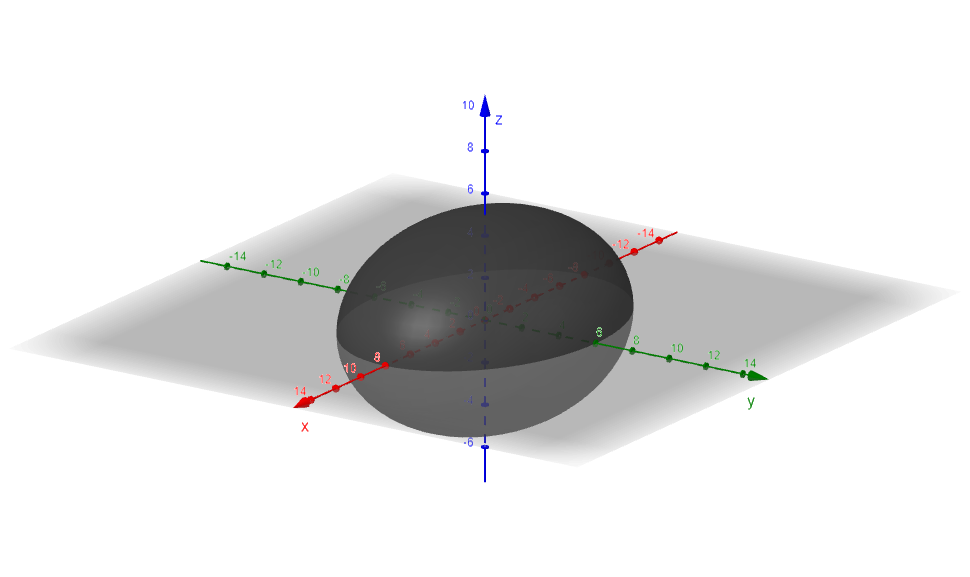
\includegraphics[width=0.75\textwidth]{Grafico_elipsoide.png}
%    \caption{Grafica de $g(x,y,z)$.}
%    \label{fig:ejemplo} % Etiqueta para hacer referencia a la imagen
%\end{figure}

\end{solution}




            \newpage
        \section{Fecha 18 de abril de 2024}
            
%----------------------------------------------------------------
\begin{question}

\vspace{1em} % Espacio vertical adicional

\begin{itemize}
    \item[a)] Calcular, si existe
    \[
        \lim_{(x,y)\to(0,0)} \frac{\sin^2{(x^{\frac{1}{3}}y)}(e^{x^2+y^2}-1)}{(x^2+y^2)^2}
    \]
     \item[b)] Calcular por definicion,
     \[
        \lim_{(x,y)\to(0,0)} \frac{3x^2+5xy^2+3y^2}{x^2+y^2}
    \]
\end{itemize}



\end{question}

%---------------------------------------------------------------------
\begin{question}
    Sea $f$ un campo escalar diferenciable en todo $\Rn{2}$ y sea $\pi:2x+3y+4z=1$ el plano tangente a la gráfica de $f$ en el punto $(1,2,f(1,2))$. Hallar todos los vectores unitarios $v$ tales que $f_v(1,2)=0.$
\end{question}
%------------------------------------------------
\begin{question}
    Analizar la diferenciabilidad de $f$ en (0,0) siendo
      \[
        f(x,y) =
        \begin{dcases}
            \frac{x^2y^2}{x^2y^2+(x-y)^2} & \textnormal{si}\ (x,y) \neq (0,0) \\
            0                         & \textnormal{si}\ (x,y) = (0,0)
        \end{dcases}
    \]
\end{question}
%------------------------------------------------------------------
\begin{question}
    Sean $g(x,y)=(xy^2,x^2-2y)$ y $h(x,y)=f \circ g(x,y)$ con $f$ de clase $C^1$ en $\Rn{2}$. Sabiendo que $h(1,-1)=2$ y que $\nabla h(1,-1)=(2,-4)$. Calcular
    \[
        \lim_{(x,y)\to (1,3)} \ 
        \frac{f(x,y)-2x+(x-1)^3}{\sqrt{(x-1)^4+(x-1)^2+(y-3)^2}}       
    \]
\end{question}
%---------------------------------------------------------------------
\newpage

\begin{solution}
    Para resolver el item a, se busca utilizar los notables conocidos de funciones del tipo $f:\R\Rightarrow\R$ para resolver el limite pedido, en primer lugar se multiplica arriba y abajo por $(x^{\frac{2}{3}}y^2)$ sabiendo que $(x,y)\neq(0,0)$
    \[
        \lim_{(x,y)\to(0,0)} \frac{\sin^2{(x^{\frac{1}{3}}y)}}{(x^{\frac{2}{3}}y^2)}\frac{(e^{x^2+y^2}-1)}{(x^2+y^2)}\frac{(x^{\frac{2}{3}}y^2)}{(x^2+y^2)}
    \]
Primero se utiliza el límite notable conocido:    
\[
        \lim_{t\to 0} \
        (\frac{e^{t}-1}{t})=1
    \]
    Llamamos  $t_1(x,y)=x^{2}+y^{2}$ y sabemos que 
   \[
        \lim_{(x,y)\to(0,0)} t_1(x,y)=0
    \]
    Definimos $g_1(z)=\frac{e^{z}-1}{z} $ y realizando la composición $f(x,y)=g_1\circ t_1(x,y) \hspace{0.25cm}\forall (x,y)\in \mathbb{R}^ 2 -(0,0)$ tenemos que
\[
        \lim_{(x,y)\to (0,0)} \
        g_1\circ t_1(x,y)=\lim_{(x,y)\to (0,0)} \
        g_1(t_1(x,y))=\lim_{t_1(x,y)\to 0} \
        \frac{e^{t_1(x,y)}-1}{t_1(x,y)}=1
    \]
En segundo lugar, se utiliza el notable conocido: 
\[
        \lim_{t\to 0} \
        \frac{\sin^2{(t)}}{t^2}=1
 \]
  Llamamos  $t_2(x,y)=x^{\frac{1}{3}}y$ y sabemos que 
   \[
        \lim_{(x,y)\to(0,0)} t_2(x,y)=0
    \]
    Definimos $g_2(z)=\frac{\sin^2{(z)}}{z^2} $ y realizando la composición $f(x,y)=g_2\circ t_2(x,y) \hspace{0.25cm}\forall (x,y)\in \mathbb{R}^ 2 -(0,0)$ tenemos que
\[
        \lim_{(x,y)\to (0,0)} \
        g_2\circ t_2(x,y)=\lim_{(x,y)\to (0,0)} \
        g_2(t_2(x,y))=\lim_{t_2(x,y)\to 0} \
        \frac{\sin^2{(t_2(x,y))}}{t_2(x,y)^2}=1
    \]

    De esta manera, se resuelve en un cálculo auxiliar el tercer término del límite solicitado
\[
        \lim_{(x,y)\to(0,0)} \frac{(x^{\frac{2}{3}}y^2)}{(x^2+y^2)}=0
    \]
Ya que podemos utilizar la propiedad de acotada por cero:
\[
        0\le y^2\le x^2+y^2    \Rightarrow   0\le \frac{y^2}{x^2+y^2}\le 1
    \]
Por lo cual, finalmente
\[
        \lim_{(x,y)\to(0,0)} \frac{\sin^2{(x^{\frac{1}{3}}y)}(e^{x^2+y^2}-1)}{(x^2+y^2)^2}=0
    \]
\newpage
Para el item b, se nos pide calcular el siguiente limite por defincion
\[
        \lim_{(x,y)\to(0,0)} \frac{3x^2+5xy^2+3y^2}{x^2+y^2}
    \]
Sabemos que:
\[
\lim_{(x,y) \to (0,0)} f(x,y) = L
\]
si, para cada \( \epsilon > 0 \), existe un \( \delta > 0 \) / \( 0 < |(x,y)| < \delta \) $\Rightarrow$ \( |f(x,y) - L| < \epsilon \).
Partimos de 
\[
|\frac{3x^2+5xy^2+3y^2}{x^2+y^2}-L|=|3+\frac{5xy^2}{x^2+y^2}-L|
\]
Propongo $L=3$, entonces
\[
|f(x,y) - L|=|\frac{5xy^2}{x^2+y^2}|=\frac{5|x|y^2}{x^2+y^2}
\]
Sabemos que 
\[
0\le x^2\le x^2+y^2 \Rightarrow 0\le |x|\le \sqrt{x^2+y^2 }
\]
\[
0\le y^2\le x^2+y^2
\]
Por lo cual
\[
\frac{5|x|y^2}{x^2+y^2} \le \frac{5(\sqrt{x^2+y^2})(x^2+y^2)}{x^2+y^2}=5(\sqrt{x^2+y^2})<5\delta
\]
Basta con tomar $\delta=\frac{\epsilon}{5}$ de manera que resulta
\[
5(\sqrt{x^2+y^2})<5\delta<\epsilon
\]
$\therefore  \lim_{(x,y)\to(0,0)} \frac{3x^2+5xy^2+3y^2}{x^2+y^2}=3$ 
\end{solution}
\newpage


%---------------------------------------------------------------------------------------------------------------------------------------

\begin{solution}
Sabemos que el plano tangente a la gráfica de $f$ en el punto $(1,2,f(1,2))$ se escribe como:
\[   
    z= f(1,2) + \nabla f(1,2)(x-1,y-2)
\]

Ademas, se nos da de dato que el plano tangente de $f$ en el punto $(1,2,f(1,2))$ es $\pi:2x+3y+4z=1$, por lo cual lo vamos a reescribir de la siguiente forma:

\[   
z= -\frac{7}{4} + (-\frac{1}{2},-\frac{3}{4})(x-1,y-2)
\]

Por lo cual sabemos que,
\[   
f(1,2)=-\frac{7}{4}
\]
\[
 \nabla f(1,2)=(-\frac{1}{2},-\frac{3}{4})
\]


    Como   $f$ es diferenciable en todo $\Rn{2}$, entonces $f$ admite todas sus derivadas direccionales en (1,2) y además, $f_v(1,2)=\nabla f(1,2).v$ / $\|\mathbf{v}\|=1$ , de esta manera definimos un $v=(v_1,v_2)$ y armamos un sistema de ecuaciones.
     y con la información de la consigna, se despejan
     
    \[\begin{cases}
            \;(-\frac{1}{2},-\frac{3}{4})(v_1,v_2)=0 \\[5pt]
            \;v_1^2+v_2^2=1
        \end{cases}
    \]
    
    De esta manera, obtenemos dos vectores resultantes:
    \[
    v=(-\frac{3}{\sqrt{13}},\frac{2}{\sqrt{13}})
    \]
     \[
    v=(\frac{3}{\sqrt{13}},-\frac{2}{\sqrt{13}})
    \]
    

\newpage
\end{solution}

\begin{solution}
   En primer lugar analizamos la continuidad, como $f$ es una función partida, queremos demostrar que $f$ es continua en (0,0) si:  $\lim_{(x,y)\to(0,0)} \ f(x,y) = f(0,0)=0$
   
    \[
        \lim_{(x,y)\to(0,0)} \
         \frac{x^2y^2}{x^2y^2+(x-y)^2}
    \]

    Este limite se analiza tomando curvas distintas:

\begin{itemize}
    \item[1)] Curva 1: $\alpha_1(t)=(0,t) / \lim_{t\to0} \alpha_1(t) = (0,0)$
    \[
         \lim_{t\to0} \
          f\circ\alpha_1(t)=\lim_{t\to0} \
         \frac{0^2t^2}{0^2t^2+(0-t)^2}\lim_{t\to0} \
          0=0
    \]

     \item[2)]  Curva 2: $\alpha_2(t)=(t,t) / \lim_{t\to0} \alpha_2(t) = (0,0)$
     \[
         \lim_{t\to0} \
          f\circ\alpha_2(t)=\lim_{t\to0} \
         \frac{t^2t^2}{t^2t^2+(t-t)^2}=\lim_{t\to0} \
         \frac{2t^2}{2t^2}=\lim_{t\to0} \
         1=1
    \]
\end{itemize}
Sabemos que $\lim_{(x,y)\to(0,0)} \ f(x,y) = L \iff \lim_{t\to0} \ f\circ\alpha(t)=L  $          $ \forall\alpha:\R\rightarrow\Rn{2}  $ 

   
De esta manera, encontramos dos curvas cuyos limites no son iguales, por lo tanto $\nexists \lim_{(x,y)\to(0,0)} \ f(x,y)$

Para responder a la consigna, utilizamos la siguiente proposicion:
 \begin{center} Si $f$ es diferenciable $\Rightarrow f$ es continua \end{center}

 Entonces, utlizando el contrareciproco: 
\begin{center}Si $f$ no es continua $\Rightarrow f$ no es diferenciable \end{center}

$\therefore f $ no es diferenciable en (0,0)
 
\end{solution}


%---------------------------------------------------------------------------------------------------------------------------------------------------

\begin{solution}
    Sean $g(x,y)=(xy^2,x^2-2y)$ y $h(x,y)=f \circ g(x,y)$ con $f$ de clase $C^1$ en $\Rn{2}$. Sabiendo que $h(1,-1)=2$ y que $\nabla h(1,-1)=(2,-4)$. Calcular
    \[
        \lim_{(x,y)\to (1,3)} \ 
        \frac{f(x,y)-2x+(x-1)^3}{\sqrt{(x-1)^4+(x-1)^2+(y-3)^2}}       
    \]

 Por un lado,      $h(1,-1)= f\circ g (1,-1) =  f(1,3)=2$  y por otro lado,  como $f$ y $g$ son ambas diferenciables,  por la regla de la cadena,  tenemos que
    \begin{equation}
        \nabla h(1,-1)=\nabla (f\circ g)(1,-1)=\nabla f(g(1,-1)) \:\boldsymbol{D}_g(1,-1) = \nabla f (1,3) \:\boldsymbol{D}_g(1,-1),  \label{eq:hNabla}
    \end{equation}    donde $\boldsymbol{D}_g$ es la matriz diferencial o  jacobiana de $g$.

    
    \noindent  Hallemos $\boldsymbol{D}_g$
    \begin{align*}
        \boldsymbol{D}_g(1,-1) & =
        \left(\begin{array}{cc}
                      \displaystyle\partialx (xy^2)            & \displaystyle\partialy (xy^2)           \\[10pt]
                      \displaystyle\partialx  (x^2 -2y) & \displaystyle\partialy (x^2 -2y)
                  \end{array}\right)\left.\rule{0pt}{1.1cm}\right\rvert_{(1,-1)}             \\[2pt]
                              & =\left(\begin{array}{cc}
                                               \displaystyle y^2                 & \displaystyle 2xy              \\[5pt]
                                               \displaystyle   2x & \displaystyle -2
                                           \end{array}\right)\left.\rule{0pt}{0.7cm}\right\rvert_{(1,-1)} \\[2pt]
                              & =\left(\begin{array}{cc}
                                               1    & -2    \\
                                               2 & -2
                                           \end{array}\right)
    \end{align*}
    Luego, reemplazando en  a   \eqref{eq:hNabla}
    \[
        \nabla h(1,-1) = \nabla f(1,3)\left(\begin{array}{cc}
                1   & -2    \\
                2 & -2
            \end{array}\right) = \left(f_x(1,3) + 2f_y(1,3),\;-2f_x(1,3)-2f_y(1,3)\right)
    \]

    y con la información de la consigna, se despejan
    \[\begin{cases}
            \;f_x(1,3) + 2f_y(1,3)=2 \\[5pt]
            \;-2f_x(1,3)- 2f_y(1,3)=-4
        \end{cases}
        \iff
        \begin{cases}
            \;f_x(1,3)=2 \\[5pt]
            \;f_y(1,3)=0
        \end{cases}
    \]
    $\therefore\quad\nabla f(1,3)=(2,0)$.

   Entonces la ecuación del plano tangente al grafico de $f$ en el punto $(1,3,f(1,3))$ es $z  = 2x$, ahora se analiza el limite solicitado separandolo en dos partes

    \[
        \lim_{(x,y)\to (1,3)} \ 
        \frac{f(x,y)-2x+(x-1)^3}{\sqrt{(x-1)^4+(x-1)^2+(y-3)^2}}
 \]
        \[
        \lim_{(x,y)\to (1,3)} \ 
        \frac{f(x,y)-2x}{\sqrt{(x-1)^4+(x-1)^2+(y-3)^2}}+ \frac{(x-1)^3}{\sqrt{(x-1)^4+(x-1)^2+(y-3)^2}} 
    \]

En primer lugar, buscamos acotar la funcion
\[
0\le (x-1)^2+(y-3)^2\le (x-1)^4+(x-1)^2+(y-3)^2
\]\[
0\le \frac{1}{\sqrt{(x-1)^4+(x-1)^2+(y-3)^2}} \le \frac{1}{\sqrt{(x-1)^2+(y-3)^2}}
\]
\[
0\le \frac{|f(x,y)-2x|}{\sqrt{(x-1)^4+(x-1)^2+(y-3)^2}} \le \frac{|f(x,y)-2x|}{\sqrt{(x-1)^2+(y-3)^2}}
\]

Ademas sabemos que $f$ es C1, que el plano tangente de $f$ en el punto (1,3) es: z=2x y que $\sqrt{(x-1)^2+(y-3)^2}=|(x-1,y-3)|$
\[
        \lim_{(x,y)\to (1,3)} \ 
        \frac{f(x,y)-2x}{\sqrt{(x-1)^2+(y-3)^2}}=0
 \]

Utilizando la regla del sandwich
\[
        \lim_{(x,y)\to (1,3)} \ 
        \frac{|f(x,y)-2x|}{\sqrt{(x-1)^4+(x-1)^2+(y-3)^2}}=0
 \]

 Y por ultimo tenemos que $  \lim_{(x,y)\to(1,3)} g(x,y)=0 \iff \lim_{(x,y)\to(1,3)} |g(x,y)|=0$, entonces
 \[
        \lim_{(x,y)\to (1,3)} \ 
        \frac{f(x,y)-2x}{\sqrt{(x-1)^4+(x-1)^2+(y-3)^2}}=0
 \]

 En segundo lugar, se analiza el segundo termino del limite
  \[
        \lim_{(x,y)\to (1,3)} \ 
       \frac{(x-1)^3}{\sqrt{(x-1)^4+(x-1)^2+(y-3)^2}} 
    \]
    Donde repetimos la misma cota que antes
    \[
0\le \frac{1}{(x-1)^4+(x-1)^2+(y-3)^2} \le \frac{1}{(x-1)^2+(y-3)^2}
\]
\[
0\le \frac{|(x-1)^3|}{(x-1)^4+(x-1)^2+(y-3)^2} \le \frac{|(x-1)^3|}{(x-1)^2+(y-3)^2}
\]
donde
\[
(x-1)^2\le(x-1)^2+(y-3)^2
\]
\[
|(x-1)|\le \sqrt{(x-1)^2+(y-3)^2}
\]
\[
|(x-1)^3|\le (\sqrt{(x-1)^2+(y-3)^2})^3
\]
de manera que
\[
0\le \frac{|(x-1)^3|}{(x-1)^4+(x-1)^2+(y-3)^2} \le \sqrt{(x-1)^2+(y-3)^2}
\]
 Utilizando el teorema del sandwich y la propiedad donde $  \lim_{(x,y)\to(1,3)} g(x,y)=0 \iff \lim_{(x,y)\to(1,3)} |g(x,y)|=0$, entonces resulta que
 \[
        \lim_{(x,y)\to (1,3)} \ 
       \frac{(x-1)^3}{\sqrt{(x-1)^4+(x-1)^2+(y-3)^2}} =0
    \]

Por lo cual, finalmente se analiza en completo el limite solicitado
 \[
        \lim_{(x,y)\to (1,3)} \ 
        \frac{f(x,y)-2x+(x-1)^3}{\sqrt{(x-1)^4+(x-1)^2+(y-3)^2}} =0      
    \]
\end{solution}

            

        \newpage
        \section{Fecha Recuperatorio 2cuatri 2022}
            %------------Ejercicio 1---------------------------------------

\begin{question}
    Sea la función

    \[
        f(x,y) =
        \begin{cases}
            \displaystyle \frac{yx^3-xy^3}{x^2+y^2} & \text{si}\; (x,y) \neq (0,0) \\[10pt]
            \qquad 0                                & \text{si}\; (x,y)=(0,0)
        \end{cases}
    \]

    probar que no existe $\delta>0$ tal que $f$ sea clase $C^2$ en $B_{\delta}(0,0)$.
\end{question}

%------------Ejercicio 2---------------------------------------

\begin{question} Calcular
    \[
        \lim_{(x,y) \to (0,0)}
        \frac{e^{2x}e^{3y} - 1 - 2x -3y - 3x^2 - 6yx - \frac{11}{2}y^2}{x^2+y^2}
    \]
\end{question}

%------------Ejercicio 3---------------------------------------

\begin{question}
    Sea $S$ el conjunto de puntos en  $\Rn{3}$  que forman la esfera de centro $(3,4,5)$ tal que el $(0,0,0) \in S$.
    \begin{itemize}
        \item [a.] Hallar el plano tangente a $S$ en $(0,0,0)$.
        \item [b.] Hallar otro plano que sea tangente a $S$ y paralelo al del ítem a.
    \end{itemize}
\end{question}

%------------Ejercicio 4---------------------------------------

\begin{question}
    Hallar los puntos de $A:(x-1)^2 + (y-1)^2 = 4$ que realicen la distancia mínima y máxima al origen.
\end{question}

\newpage
%-----------Solucion 1--------------------------------------------

\begin{solution}
    Por el teorema de Schwartz sabemos que si $f \in\ C^2$ en  $B_{\delta}(0,0)$
    entonces $$  f_{xy} (x,y) = f_{yx} (x,y) \quad \forall (x,y) \in B_{\delta}(0,0).$$ En particular, deber\'ia pasar que $f_{xy} (0,0) = f_{yx}(0,0).$ Veamos que esto \'ultimo no sucede.

    \begin{equation}
        f_x(x,y) = \frac{(3yx^2-y^3)(x^2+y^2) - (yx^3-xy^3)2x}{(x^2+y^2)^2} \label{eq:partXej1}
    \end{equation}

    \begin{equation}
        f_y(x,y) = \frac{(x^3-3xy^2)(x^2+y^2) - (yx^3-xy^3)2y}{(x^2+y^2)^2}  \label{eq:partYej1}
    \end{equation}

    Para $(x,y) = (0,0)$, calculamos las derivadas por definición.
    \[
        f_x(0,0)  = \lim_{h\to0} \frac{f(h,0) - f(0,0)}{h} = 0
    \]
    \[
        f_y(0,0)  =  \lim_{h\to0} \frac{f(0,h) - f(0,0)}{h} = 0
    \]

    Ya tenemos definidas las derivadas parciales de $f$ en todo $\Rn{2}.$
    \[
        f_x(x,y) =
        \begin{cases}
            \eqref{eq:partXej1} & \text{si}\ (x,y) \neq (0,0) \\
            0                   & \text{c.c.}
        \end{cases}
    \]

    \[
        f_y(x,y) =
        \begin{cases}
            \eqref{eq:partYej1} & \text{si}\ (x,y) \neq (0,0) \\
            0                   & \text{c.c.}
        \end{cases}
    \]

    Ahora podemos calcular las derivadas parciales cruzadas de segundo orden por definición.

    \begin{equation}
        f_{xy}(0,0) = \lim_{h\to0} \frac{f_x(0,h) - f_x(0,0)}{h} \label{eq:limDef1}
    \end{equation}

    \begin{equation}
        f_{yx}(0,0) = \lim_{h\to0} \frac{f_y(h,0) - f_y(0,0)}{h}  \label{eq:limDef2}
    \end{equation}

    Por \eqref{eq:partXej1} y \eqref{eq:partYej1}, se puede observar que
    \[
        f_x(0,h) = -h \text{ y } f_y(h,0) = h.
    \]

    Entonces por \eqref{eq:limDef1} Y \eqref{eq:limDef2}
    \[
        f_{xy}(0,0) = -1 \neq f_{yx}(0,0) = 1.
    \]

    $\therefore\;$ no existe $\delta>0$ tal que $f$ sea clase $C^2$ en $B_{\delta}(0,0)$.
\end{solution}

%-----------Solucion 2--------------------------------------------

\begin{solution}
    Para resolverlo debemos intuir que está conformado por el límite de buena aproximación de un polinomio de Taylor de segundo orden centrado en el origen de una función. Buscamos una expresión para dicho polinomio y para la función.

    Llamemos $f(x,y) = e^{2x}e^{3y}$, notemos que $f$ es de clase $C^3(\Rn{2}).$  Entonces, podemos definir su polinomio de Taylor de segundo orden centrado en el origen, $ P_2(x,y)$, y adem\'as vale el teorema de resto de Taylor
    \[
        P_2(x,y) = f(0,0) + \nabla f(0,0)\cdot(x,y) + \frac{1}{2}(x,y)\boldsymbol{H}_f(0,0)(x,y)^\mathrm{T},
    \]
    siendo $\boldsymbol{H}_f(0,0)$ la matriz hessiana de $f$ evaluada en el origen.

    Tenemos que
    \begin{gather*}
        f(0,0) = 1,\\[.2cm]
        \nabla f(x,y) = \left(2e^{2x}e^{3y}, 3e^{2x}e^{3y}\right) \implies \nabla f(0,0) = (2,3),\\[.25cm]
        \boldsymbol{H}_f(x,y) = \left(\begin{array}{cc}
                4e^{2x}e^{3y} & 6e^{2x}e^{3y} \\[10pt]
                6e^{2x}e^{3y} & 9e^{2x}e^{3y}
            \end{array}\right) \implies \boldsymbol{H}_f(0,0) = \left(\begin{array}{cc}
                4 & 6 \\
                6 & 9
            \end{array}\right).
    \end{gather*}
    Entonces queda
    \[
        \begin{aligned}
            P_2(x,y)      & = 1+(2,3)\cdot(x,y)+\frac{1}{2}(x,y)
            \left(\begin{array}{cc}  
                    4 & 6 \\
                    6 & 9
                \end{array}\right)
            \left(\begin{array}{cc}
                          x \\
                          y
                      \end{array}\right)                                                     \\[4pt]
            \iff P_2(x,y) & = 1 + 2x + 3y + 2x^2 + 6xy + \frac{9}{2}y^2.
        \end{aligned}
    \]
    Expresamos el error como
    \[
        R_2(x,y) = f(x,y) - P_2(x,y).
    \]
    Por tanto, podemos reescribir el límite original como
    \[\\[2pt]
        \lim_{(x,y) \to (0,0)} \frac{R_2(x,y) - x^2 - y^2}{\|(x,y)\|^2} =
        \lim_{(x,y) \to (0,0)} \left( \frac{R_2(x,y)}{\|(x,y)\|^2} - \frac{x^2+y^2}{\|(x,y)\|^2} \right) = -1,
    \]
    pues el primer término tiende a 0 por el teorema de Taylor  y el segundo  tiende claramente a $1.$
\end{solution}

%-----------Solucion 3--------------------------------------------

\begin{solution}
    a. Dado que el origen pertenece a $S$ y conocemos su centro, podemos hallar la ecuación de la esfera.
    \[
        S:(x-3)^2 + (y-4)^2 + (z-5)^2 = 50
    \]
    \begin{center}
        \begin{tikzpicture}
            \begin{axis}[
                    view={70}{15},
                    axis equal,
                    width=14cm,
                    height=12cm,
                    axis lines = center,
                    xlabel = {$x$},
                    ylabel = {$y$},
                    zlabel = {$z$},
                    zmin=-1,
                    xmin=-1,
                    ymin=-1,
                    zmax=14,
                    xmax=14,
                    ymax=12,
                    colormap/viridis
                    % ticks=none,
                ]
                \addplot3[
                    surf,
                    opacity=0.5,
                    samples=21,
                    domain=0:360,
                    y domain=0:180,
                    z buffer=sort
                ]
                ({3 + sqrt(50) * sin(y) * cos(x)},
                {4 + sqrt(50) * sin(y) * sin(x)},
                {5 + sqrt(50) * cos(y)});

            \end{axis}
        \end{tikzpicture}
    \end{center}

    Llamando $$f:\mathbb{R}^3 \rightarrow \mathbb{R}:  f(x,y,z) = (x-3)^2 + (y-4)^2 + (z-5)^2 - 50$$
    tenemos que $$S=C(f,0). $$
    Buscamos el plano $\Pi$, tangente a $C(f,0)$ y que pase por $(0,0,0)$. Sabemos que la ecuación de  $\Pi$  es  de la forma
    \[
        \Pi:\nabla f(0,0,0) \cdot (x-0,y-0,z-0) = 0.
    \]
    Es f\'acil ver que $\nabla f(0,0,0) = (-6,-8,-10).$  Luego, una posible ecuaci\'on es
    \[\\[1pt]
        \Pi: 3x + 4y + 5y = 0.
    \]

    b. Dado que el único plano paralelo a otro tangente a un punto en una esfera es el que se encuentra en el polo opuesto de ésta, buscamos el plano tangente $\Pi'$ a ese otro punto $\mathbf{w}$. Llamando $\mathbf{v} = (-3,-4,-5)$ al vector que sale del centro de la esfera y termina en el origen, queda que
    \[
        \mathbf{w} = (3,4,5) - \mathbf{v} = (6,8,10).
    \]
    Como $\Pi$ y $\Pi'$ son paralelos, su vector normal $\textbf{n}$ es el mismo.
    \[
        \begin{aligned}
            \implies & \Pi ': \textbf{n} \cdot ((x,y,z) - \mathbf{w}) = 0 \\
            \iff     & \Pi ': 3(x-6) + 4(y-8) + 5(z-10) = 0               \\
            \iff     & \Pi ':3x + 4y + 5y = 100
        \end{aligned}
    \]

    \begin{center}
        \begin{tikzpicture}
            \begin{axis}[
                    view={60}{7},
                    axis equal,
                    width=14cm,
                    height=14cm,
                    axis lines = center,
                    xlabel = {$x$},
                    ylabel = {$y$},
                    zlabel = {$z$},
                    zmin=-20,
                    xmin=-10,
                    ymin=-10,
                    zmax=30,
                    xmax=40,
                    ymax=30,
                    colormap/viridis
                ]

                % Add the second plane
                \addplot3[
                    surf,
                    fill = blue,
                    opacity=0.6,
                    domain=-10:15,
                    y domain=-10:15,
                ]
                {- (3*x + 4*y)/5}; % Equation of the second plane: 3x + 4y + 5z = 0

                \addplot3[
                    surf,
                    opacity=0.5,
                    samples=21,
                    domain=0:360,
                    y domain=0:180,
                    z buffer=sort
                ]
                ({3 + sqrt(50) * sin(y) * cos(x)},
                {4 + sqrt(50) * sin(y) * sin(x)},
                {5 + sqrt(50) * cos(y)});

                % Add the first plane
                \addplot3[
                    surf,
                    fill = red,
                    opacity=0.6,
                    domain=-10:15,
                    y domain=-10:15,
                ]
                {20-(3*x + 4*y)/5}; % Equation of the first plane: 3x + 4y + 5z = 100

            \end{axis}
        \end{tikzpicture}
    \end{center}
\end{solution}


\vspace{0.3 cm}

%-----------Solucion 4--------------------------------------------

\begin{solution}
    Sean
    \[
        f: \mathbb{R}^2 \rightarrow \mathbb{R}, \; f(x,y) = \text{dist}^2\Big((x,y);(0,0)\Big)  = x^2 + y^2
    \]
    y
    \[
        g: \mathbb{R}^2 \rightarrow \mathbb{R}, \; g(x,y) = (x-1)^2 + (y-1)^2 - 4,
    \]
    luego $A=C(g,0) $.

    Como $f,g \in C^1( \mathbb{R}^1),$  el teorema de los multiplicadores de Lagrange nos dice que si $f \big\rvert _A$ tiene un extremo local en un punto \textbf{x} entonces necesariamente los vectores $\nabla f(\textbf{x})$ y $\nabla g(\textbf{x})$ son paralelos si $\nabla g(\textbf{x}) \neq 0$.   Además como $f$ es continua sobre el conjunto $A$ que es cerrado y acotado, por el teorema de Weierstrass, sabemos que $f$ alcanza m\'aximo y m\'inimo en $A$. Luego planteamos el siguiente sistema de ecuaciones
    \[
        \nabla f(x,y) = \lambda \nabla g(x,y), \; \lambda \in \mathbb{R}, \; (x,y) \in A \\
        \iff \begin{cases}
            2x = 2\lambda(x-1) \\
            2y = 2\lambda(y-1) \\
            (x-1)^2 + (y-1)^2 = 4
        \end{cases}
    \]
    Resolviendo el sistema queda $x=y$  \;  y \[ \begin{cases}
            x=   x_1=1+\sqrt{2} \\
            x=  x_2=1-\sqrt{2}.
        \end{cases}\]
    $\implies (x_1,x_1)$  y $(x_2,x_2)$  son ambos extremos absulutos de la función $f$  en $A$. Como $f(x_1,x_1) > f(x_2,x_2) \implies (x_1,x_1)$ es máximo absoluto y $(x_2,x_2)$ es mínimo absoluto.

    Luego  la distancia mínima del circulo al origen es $\sqrt{f(x_2,x_2)} = 2-\sqrt{2} $ y la distancia máxima $\sqrt{f(x_1,x_1)} = 2+\sqrt{2}$.
\end{solution}




        \newpage
    \chapter{Segundos parciales resueltos}
        \section{Fecha 25 de junio de 2023}
            %------------Ejercicio 1---------------------------------------

\begin{question}
    Sea  $S$  la superficie dada por $x^{2}+ y^{2} = z$ con $z \geq 1$  y $x^{2}+ y^{2} \leq 4$  y sea  $\mathbf{F}:\mathbb{R}^{3}\rightarrow\mathbb{R}^{3}$  un campo de clase $C^{1}$ con tercer componente  nula y $\nabla \cdot \mathbf{F}$ constante 3. Calcular el flujo de  $\mathbf{F}$  a trav\'es de $S$ indicando la orientaci\'on elegida.
\end{question}

%------------Ejercicio 2---------------------------------------

\begin{question}
    Sea $\mathbf{F}(x,y,z) = (y^{2}-2xz,\;2xy+z^{3},\;3yz^{2}-x^{2}) $ y sea  $C$ una curva simple parametrizada por $\boldsymbol{\sigma}:[0,1]\rightarrow \mathbb{R}^{3}$
tal que $\boldsymbol{\sigma}(0)=(0,0,0)$ y $\boldsymbol{\sigma}(1)=(1,2,0)$. Calcular $\int_{C} \mathbf{F}\cdot d\mathbf{s}$ indicando la orientaci\'on elegida. 
\end{question}

%------------Ejercicio 3---------------------------------------

\begin{question}
    Calcular la masa del cuerpo limitado por las ecuaciones $y-x=1$ y $x^{2}+ z^{2} = 1$ en el primer octante con funci\'on de densidad $\rho$ constante.  
\end{question}

%------------Ejercicio 4---------------------------------------

\begin{question}
     Sean  $k\in\mathbb{R}$,  un campo vectorial $\mathbf{F}:\mathbb{R}^{2}\rightarrow\mathbb{R}^{2}$   de clase $C^{1}$ tal que $\nabla\times \mathbf{F}=k$ y $D=\{ (x,y) \in \mathbb{R}^{2} :  |x| \leq 1 \:  ; \:   x \leq y\leq 1  \}.$ Hallar $k$ tal que $\int_{\partial D^{+}}\mathbf{F}\cdot d\mathbf{s} = 8$. 
\end{question}

%------------Solucion 1---------------------------------------
\newpage
\begin{solution}
    Es \'util primero entender con qu\'e superficies y regiones se trabajar\'a.
    % \begin{center}
    % \begin{tikzpicture}
    %     \begin{axis}[
    %         view={60}{20}, % ajusta el angulo de vision
    %         xlabel=$x$,
    %         ylabel=$y$,
    %         zlabel=$z$,
    %         zmin=0, % valor minino del eje z
    %         zmax=5, % valor maximo del eje z
    %         axis lines=center, % sin caja solo ejes
    %         ticks=none, % ejes sin marcas
    %         width=10cm,
    %         height=12cm,
    %         enlargelimits=0.2, % ajuste de limite de vision
    %         domain=-3:3,
    %         y domain=-3:3,
    %         samples=30, % numero de cuadrados por simulacion (esto aumenta el tiempo de compilacion drasticamente)
    %         colormap/cool, % color
    %     ]
    %     \addplot3 [surf, opacity=0.5, draw=none, restrict z to domain=1:4, 
    %     data cs=polar, domain=0:360, y domain=0:4] (x, y, y^2);
    
    %     \end{axis}
    % \end{tikzpicture}
    % \end{center}
    \begin{center}
    \begin{tikzpicture}
        \begin{axis}[
            view={60}{20},
            xlabel=$x$,
            ylabel=$y$,
            zlabel=$z$,
            xmin=-2.5,
            ymin=-2.5,
            zmin=0,
            xmax=2.5,
            ymax=2.5,
            zmax=5,
            samples=30,
            width=10cm,
            height=12cm,
            colormap/viridis,
        ]
        \addplot3 [surf, opacity=0.8, draw=none, restrict z to domain=1:4, 
        data cs=polar, domain=0:360, y domain=0:4] (x, y, y^2);
        \end{axis}
    \end{tikzpicture}
    \end{center}
            
   La idea es aplicar el teorema de Gauss pero  $S$ no es una superficie cerrada.   Para ello pensemos en una superficie $S'$  cerrada tal  que $S \subseteq S'.$  Definamos   $S'=S\;\cup\;S_1\;\cup\;S_2$,  donde $S_1$ y $S_2$, son las ``tapas'' del paraboloide ``cortado''.  Algebraicamente $S_1=\{(x,y,z)\in \Re^3 : x^2+y^2\le 1\;\land z=1\}$ y $S_2=\{(x,y,z)\in \Re^3 : x^2+y^2\le4\;\land z=4\}$.
    
  Llamando  $\Omega$  al cuerpo encerrado por $S'$ y orientando a $S'$ de manera exterior estamos en condiciones de usar el teorema de Gauss.
    \begin{gather*}
        \oiint _{S'} \mathbf{F}\cdot d\mathbf{A} =
        \iint _{S} \mathbf{F}\cdot d\mathbf{A} +
        \iint _{S_1} \mathbf{F}\cdot d\mathbf{A} +
        \iint _{S_2} \mathbf{F}\cdot d\mathbf{A} 
        =\iiint _\Omega \nabla \cdot \mathbf{F}\;dV\\[.2cm]
        \iff \iint _{S} \mathbf{F}\cdot d\mathbf{A} =
        \iiint _\Omega \nabla \cdot \mathbf{F}\;dV -
        \iint _{S_1} \mathbf{F}\cdot d\mathbf{A} -
        \iint _{S_2} \mathbf{F}\cdot d\mathbf{A}\\[.2cm]
        \iff \iint _{S} \mathbf{F}\cdot d\mathbf{A} = 
        I_1-I_2-I_3
    \end{gather*}

    Resolvemos el primer t\'ermino.
    \begin{align*}
        I_1=\iiint _\Omega \nabla \cdot \mathbf{F}\;dV = \iiint _\Omega3\:dV = 3\:\text{Vol}(\Omega)
    \end{align*}
    Pasando a  $\Omega$ en coordenadas cil\'indricas
    \[\begin{dcases}
        x=\rho \cos \phi\\
        y=\rho \sen \phi\\
        z=z
    \end{dcases}\] donde, $$0\leq\rho\leq \sqrt{z}\:\land\:0\leq\phi\leq 2\pi \land 1\leq z \leq 4.$$
    
    Entonces nos queda
    \[
   \text{Vol}(\Omega) =  \int_1^4  \int_0^{2\pi} \int_0^{\sqrt{z}}  \rho\:d\rho\:d\phi \:dz=2\pi  \int_1^4 \Big( \frac{\rho^2}{2}\Big|_0^{\sqrt{z}} \Big) \:dz =  \pi   \int_1^4   z  \:dz= \frac{15 \pi}{2}.  
    \] Luego, $I_1 =  \frac{45}{2}\pi. $



    Para clacular $I_2$  debemos parametrizar $S_1$.  Sea  $D_1=\{(u,v)\in\Re^2:u^2+v^2\leq1\}$ y  sea  $$\boldsymbol{\Sigma}:D_1\subset\Re^2\to\Re^3  \mbox{ tal que }   \boldsymbol{\Sigma}(u,v)=(u,v,1).$$ 
    Entonces podemos reescribir
    \[
    I_2=\iint _{D_1} (\mathbf{F}\circ\boldsymbol{\Sigma})\cdot
    (\boldsymbol{\Sigma}_u\times\boldsymbol{\Sigma}_v)\:d\mathbf{A}.
    \]
    Primero calculamos las derivadas parciales de la parametrizaci\'on.
    \begin{align*}
    \boldsymbol{\Sigma}_u&=(1,0,0)\\
    \boldsymbol{\Sigma}_v&=(0,1,0)
    \end{align*}
    Entonces
    \[
    \boldsymbol{\Sigma}_u\times\boldsymbol{\Sigma}_v=(0,0,1)=\boldsymbol{\eta}.
    \]
    Podemos observar que $\boldsymbol{\eta}$ no preserva la orientaci\'on  para $S_1$ heredada  por la orientaci\'on exterior de $S'$ elegida anteriormente para poder aplicar el teorema de Gauss. En otras palabras,  $\boldsymbol{\eta}$ ``apunta''  hacia el interior de $\Omega$.  Por lo que,
    \[
    I_2=-\iint _{D_1} (\mathbf{F}\circ\boldsymbol{\Sigma})\cdot \boldsymbol{\eta}\:d\mathbf{A}.
    \]
    Calculamos el integrando aparte. Acord\'emonos que la tercer coordenada de $\mathbf{F}$ es nula. Podemos llamar
    \[
    \mathbf{F}\circ\boldsymbol{\Sigma}=(P,Q,0),
    \]
    entonces nos queda que
    \[
    (\mathbf{F}\circ\boldsymbol{\Sigma})\cdot \boldsymbol{\eta}=(P,Q,0)\cdot (0,0,1)=0.
    \]
    Por lo tanto $I_2=0$.
    
    Procediendo de la misma manera nos daremos cuenta que tambi\'en $I_3=0$.

    $$\therefore\;\iint _{S} \mathbf{F}\cdot d\mathbf{A}=I_1=\frac{45}{2}\pi$$
\end{solution}

%------------Solucion 2---------------------------------------

\begin{solution}
   Busquemos, si existe,  una funci\'on potencial para $\mathbf{F},$ es decir, buscamos $f$ tal que $\nabla f = F.$ Para ello,  planteamos el sistema de tres ecuaciones diferenciales dado por:
    \[\begin{dcases}
        y^2-2xz=f_x\\
        2xy+z^3=f_y\\
        3yz^2-x^2=f_z
    \end{dcases}\]
    Entonces 
    \begin{equation}
    \int f_x(x,y,z)\:dx=y^2x-zx^2+g(y,z)=f(x,y,z), \label{eq:cons1}
    \end{equation}
    donde $g$ es la constante con respecto a $x$ producto de la integraci\'on. Derivando \ref{eq:cons1} con respecto a $y$ obtenemos 
    \begin{gather*}
     f_y(x,y,z)= 2yx+g_y(y,z)\\[.2cm]
     2yx+g_y(y,z)  = 2xy+z^3 \implies g_y(y,z)=z^3\\[.2cm]
    g(y,z)=\int  g_y(y,z) \:dy =  z^3y+h(z).
    \end{gather*}
Reemplazando en  la ecuaci\'on \ref{eq:cons1},
\begin{equation}
    y^2x-zx^2+z^3+h(z) =  f(x,y,z).   \label{eq:cons2}
\end {equation}  

Derivando \ref{eq:cons2} con respecto a $z$ obtenemos 
 \begin{gather*}
 f_z(x,y,z)=-x^2+3yz^2+h_z(z)\\ 
 -x^2+3yz^2+h_z(z)=3yz^2-x^2   \implies h_z(z) =0 \\[.2cm]
   h(z) = C,  \quad\text{con}\;\;C\in\Re.
    \end{gather*}
    Por lo tanto llegamos a una familia de soluciones.
    \[
    f(x,y,z)=y^2x-zx^2+z^3+C  \quad\text{con}\;\;C\in\Re
    \]
   Demostramos que $\mathbf{F}$ es un campo conservativo pues $\mathbf{F}=\nabla f.$ Luego, podemos calcular
    \[
    \int _{\boldsymbol{\sigma}} \mathbf{F}\cdot d\mathbf{s}=
    \int _{\boldsymbol{\sigma}} \nabla f\cdot d\mathbf{s} = f(\boldsymbol{\sigma}(1))-f(\boldsymbol{\sigma}(0))=f(1,2,0)-f(0,0,0)=4.
    \]
\end{solution}

%------------Solucion 3---------------------------------------

\begin{solution}
    La masa de un cuerpo de volumen $\Omega$ es 
    \[
    M=\iiint_\Omega \rho\:dV.
    \]
    En este caso
    \[
    \Omega=\{(x,y,z)\in\Re^3:x^2+z^2\leq1\;\land\;y\leq1+x\; \land\;x,y,z\geq0\}.
    \]
    Conviene trabajar en coordenadas cil\'indricas. Sea
    \[\begin{dcases}
        x=r\sen\phi\\
        y=y\\
        z=r\cos\phi.
    \end{dcases}\]
    Entonces en el nuevo sistema de coordenadas
    \[
        \Omega^*=\{(r,\phi,y)\in\Re^3:    0\leq  r\leq1\; \land\; 0 \leq y\leq1+r\sen\phi\;\land\;  0\leq\phi\leq\frac{\pi}{2}\}.
    \]
   
    Ahora podemos reescribir, dado que $\rho$ es constante,
    \begin{align*}
  \frac{M}{\rho} =& \iiint_{\Omega^*} r\:dy\:d\phi\:dr=\int_0^1 \int_0^{\frac{\pi}{2}} \int_0^{1+r\sen\phi} r\:dy\:d\phi\:dr\\[.2cm]
    =&\int_0^1 \int_0^{\frac{\pi}{2}}r(1+r\sen\phi)\:d\phi\:dr=\int_0^1 \int_0^{\frac{\pi}{2}} ( r+r^2\sen\phi) \:d\phi\:dr\\[.2cm]
    =&\int_0^1\int_0^{\frac{\pi}{2}} r\:d\phi\:dr+\int_0^1\int_0^{\frac{\pi}{2}}r^2\sen\phi\:d\phi\:dr\\[.2cm]
    =&\int_0^1r\:dr\int_0^{\frac{\pi}{2}}d\phi+\int_0^1r^2\:dr\int_0^{\frac{\pi}{2}}\sen\phi\:d\phi\\[.2cm]
    =&\frac{\pi}{4}+\frac{1}{2}.
    \end{align*}
    \[
    \therefore\:M=\rho\left(\frac{\pi}{4}+\frac{1}{2}\right)
    \]
\end{solution}

%------------Solucion 4---------------------------------------

\begin{solution}
    La regi\'on $D$ se grafica de la siguiente manera.

    \begin{center}
    \begin{tikzpicture}
        \begin{axis}[
            axis lines=center,
            axis equal,
            xlabel=$x$,
            ylabel=$y$,
            xmin=-1,
            xmax=1,
            ymin=-1,
            ymax=1.2,
            xtick distance=1,
            ytick distance=1,
            ]
            \addplot[name path=A, draw=none]{x} node[pos=0.55, right]{$y=x$};
            \addplot[name path=B, draw=none]{1};
            \addplot[fill=violet!90, opacity=0.7]fill between[of=A and B, soft clip={domain=-1:1}];
        \end{axis}
    \end{tikzpicture}
    \end{center}


    Podemos observar que $D$ es simplemente conexo y que $\partial D$ es una curva simple cerrada, por lo tanto vale el teorema de Green.
    \[
    \oint_{\partial D^+} \mathbf{F}\cdot d\mathbf{s}=\iint_D \nabla\times\mathbf{F}\cdot d\mathbf{A}=k\iint_DdA=8,
    \]
 
  Nos quedar\'ia calcular el  $\textcolor{red}{A(D)}$,  \'area de $D$, que, por ser un tri\'angulo, se puede calcular simplemente.
    \[
    A(D) = \iint_D dA=\frac{4}{2}=2
    \]
    Entonces nos queda
    \[
    2k=8\iff k=4.
    \]
\end{solution}

        \newpage
        \section{Fecha recuperatorio 29 de junio de 2023}
            %------------------Ejercicio 1--------------------------------

\begin{question}
  Sea  $S$  la superficie dada por $x^{2}+ y^{2} = z$ con $z \geq 2$  y $x^{2}+ y^{2} \leq 9.$  Calcular el \'area de $S.$
\end{question}

%------------------Ejercicio 2--------------------------------

\begin{question}
  Sea $C$ la curva simple definida por la intersecci\'on de las superficies $x^{2}+z^{2}=16$,  $y+z=4$ con $y\leq 4$ y sea $g$ una funci\'on escalar $C^{1}(\mathbb{R})$. Calcular la integral sobre $C$ del campo $\mathbf{F}(x,y,z)=(x,\;g(y),\;g(z)).$ Indicar la orientaci\'on elegida.
\end{question}

%------------------Ejercicio 3--------------------------------

\begin{question}
  Sean $\mathbf{F}(x,y,z)=(-xy+yz,\;-y^{2}+xz,\; xz)$, $a \in \mathbb{R}$ positivo  y $S$ la superficie de seis caras que encierra el cuerpo dado por $0\leq x \leq  a$, $0 \leq  y \leq  a $ y  $0 \leq  z \leq a$ orientada con normales exteriores.   Hallar $a$ de manera que el flujo de $\mathbf{F}$ a trav\'es  de $S$ sin su cara superior sea $-24$.
\end{question}

%------------------Ejercicio 4--------------------------------

\begin{question}
  Calcule la masa del cuerpo definido por $z\leq \sqrt{x^{2} + y^{2} }$,  $x^{2} + y^{2} + z^{2} \leq 32$,  en el primer octante, si su densidad es proporcional a la distancia de un  punto al plano $z=0.$
\end{question}

\newpage

%------------------Solucion 1--------------------------------

\begin{solution}
  $S$ es una secci\'on de paraboloide, como se puede observar en el siguiente gr\'afico.

  \begin{center}
    \begin{tikzpicture}
      \begin{axis}[
          view={60}{15},
          xlabel=$x$,
          ylabel=$y$,
          zlabel=$z$,
          xmin=-2.5,
          ymin=-2.5,
          zmin=0,
          xmax=2.5,
          ymax=2.5,
          zmax=10,
          samples=30,
          width=10cm,
          height=14cm,
          colormap/viridis,
        ]
        \addplot3 [surf, opacity=0.8, draw=none, restrict z to domain=2:9,
          data cs=polar, domain=0:360, y domain=0:4] (x, y, y^2);
      \end{axis}
    \end{tikzpicture}
  \end{center}

  Escribimos el conjunto $S$ como
  \[
    S=\{(x,y,z)\in \Re^3: x^2+y^2=z;\;2\leq z\leq 9 \}.
  \]
  Queremos calcular \[ \textcolor{red}{A}(S) = \iint_S dA.\]
  Para ello necesitaremos una parametrizaci\'on de $S$. Sea
  $$D=\{(\rho, \phi) \in\Re^2:    \sqrt{2}\leq \rho \leq 3;\;0\leq  \phi \leq 2\pi \}$$  y  sea  $$\boldsymbol{\Sigma}:D \subset\Re^2\to\Re^3  \mbox{ tal que }   \boldsymbol{\Sigma}(\rho, \phi)=(\rho \cos\phi, \rho \sen\phi , \rho^{2}).$$

  Primero calculamos las derivadas parciales de la parametrizaci\'on.
  \begin{align*}
    \boldsymbol{\Sigma}_{\rho} & =(\cos \phi,\;\sen \phi,\; 2\rho)         \\
    \boldsymbol{\Sigma}_\phi   & =(  -\rho \sen \phi,\;\rho \cos \phi,\;0)
  \end{align*}
  Entonces
  $$
    \boldsymbol{\Sigma}_{\rho} \times\boldsymbol{\Sigma}_\phi =
    (-2\rho^2 \cos\phi  , \;-2\rho^2 \sen \phi, \;\rho),
  $$
  $$\|  \boldsymbol{\Sigma}_{\rho} \times\boldsymbol{\Sigma}_\phi\|
    = \rho\sqrt{4\rho^2+1}.$$
  Quedando
  \begin{equation}
    \iint_S dA
    = \int_0^{2\pi} \int_{\sqrt{2}}^3 \|\boldsymbol{\Sigma}_{\rho}
    \times\boldsymbol{\Sigma}_\phi \| \; d\rho d\phi
    = \int_0^{2\pi} \int_{\sqrt{2}}^3 \rho\sqrt{4\rho^2+1}\;d\rho d\phi,
    \label{eq:integral1}
  \end{equation}
  \begin{gather*}
  u=4\rho^2+1 \rightarrow du = 8\rho\;d\rho, 
  \\[.2cm]
  = \frac{1}{8}\int_0^{2\pi} \int_9^{37} \sqrt{u}\;du d\phi
  = \frac{2\pi}{8}\frac{u^{\frac{3}{2}}}{\frac{3}{2}}\Bigg|_9^37
  = \frac{\pi}{4\frac{3}{2}} (9^{\frac{3}{2}} - 2^{\frac{3}{2}}) 
  \\[.2cm]
  = \frac{\pi}{6} (\sqrt{9^3} - \sqrt{8}).
  \end{gather*}
\end{solution}

%------------------Solucion 2--------------------------------

\begin{solution}

  \textcolor{red}{(insertar imagen)}

  Notemos que $C$ es una curva no cerrada. Para cerrarla, llamemos $C=C_1$, 
  $C_2=\{(x,y,z)\in\Re^3:z=0\;\land\;y=4\;\land\;|x|\leq4\}$ y $C_0=C_1+C_2$. Y sea $\text{int}(C_0)=D$. Ahora $C_0$ es una curva simple cerrada. Entonces podemos aplicar el teorema de Stokes, eligiendo la orientaci\'on de $C_0$ tal que se cumpla la regla de la mano derecha.
  \[
      \oint_{C_0}\mathbf{F}\cdot d\mathbf{s}= \int_{C_1}\mathbf{F}\cdot d\mathbf{s} + \int_{C_2}\mathbf{F}\cdot d\mathbf{s} = \iint_D \nabla\times\mathbf{F}\cdot d\mathbf{A},
  \]
  ya que $\mathbf{F}$ es $C^1(\Re)$, pues sus componentes son $C^1(\Re)$, y $D\in\text{dom}(\mathbf{F})$.
  Notemos que $\nabla\times\mathbf{F}\equiv0\implies$
  \[
     \int_{C_1}\mathbf{F}\cdot d\mathbf{s} =- \int_{C_2}\mathbf{F}\cdot d\mathbf{s}.
  \]
  Ahora busquemos una trayectoria de $C_2$ que respete su orientaci\'on. Sea $\boldsymbol{\sigma}:[-4,4]\rightarrow\Re^3$
  tal que $\boldsymbol{\sigma}(t)=(t,4,0)$. Entonces $\boldsymbol{\sigma}'(t)=(1,0,0)$. Luego la integral de curva de $C_2$ es
  \begin{gather*}
    \int_{C_2}\mathbf{F}\cdot d\mathbf{s}
    =\int_{-4}^4 (\mathbf{F}\circ\boldsymbol{\sigma})\cdot\boldsymbol{\sigma}'\:dt
    =\int_{-4}^4 t\:dt = 0.
  \end{gather*}
  $\therefore$ la integral sobre la curva original $C=C_1$ es tambi\'en 0.
\end{solution}

%------------------Solucion 3--------------------------------

\begin{solution}
  Llamemos $\Omega$ al volumen que encierra $S$ y sea $S'$ la superficie de la cara superior de $S$, por lo que $S'$ tiene orientaci\'on igual que la tapa de $S$. En los siguientes gr\'aficos se puede ver la representaci\'on de $S$ y $S'$ respectivamente.

  \begin{tikzpicture}
    \begin{axis}[
        axis equal,
        axis lines = center,
        height = 11cm, width = 11cm,
        view={120}{20},
        xlabel={$x$},
        ylabel={$y$},
        zlabel={$z$},
        zmin = -1, zmax = 3,
        xmin = -1, xmax = 3,
        ymin = -1, ymax = 3,
        xtick = {0, 2},
        xticklabels = {$0$, $a$},
        ytick = {0, 2},
        yticklabels = {$0$, $a$},
        ztick = {0, 2},
        zticklabels = {$0$, $a$},
        xlabel style={at={(axis cs:3,0,0)}, anchor=north west},
        xticklabel style={anchor=north west},
        ylabel style={at={(axis cs:0,3.1,0.05)}},
        yticklabel style={at={(axis cs:0,2,0)}},
      ]

      \addplot3[fill=magenta!80, opacity=0.8, draw=none] coordinates {(0,0,0) (0,2,0) (2,2,0) (2,0,0) (0,0,0)};
      \addplot3[fill=magenta!70, opacity=0.8, draw=none] coordinates {(0,0,0) (0,0,2) (2,0,2) (2,0,0) (0,0,0)};
      \addplot3[fill=magenta!60, opacity=0.8, draw=none] coordinates {(0,0,0) (0,2,0) (0,2,2) (0,0,2) (0,0,0)};
      \addplot3[fill=magenta!65, opacity=0.8, draw=none] coordinates {(2,0,0) (2,2,0) (2,2,2) (2,0,2) (2,0,0)};
      \addplot3[fill=magenta!50, opacity=0.8, draw=none] coordinates {(0,2,0) (0,2,2) (2,2,2) (2,2,0) (0,2,0)};
      \addplot3[fill=cyan!50, opacity=0.8, draw=none] coordinates {(0,0,2) (0,2,2) (2,2,2) (2,0,2) (0,0,2)};
    \end{axis}
  \end{tikzpicture}
  \hfill
  \begin{tikzpicture}
    \begin{axis}[
        axis equal,
        axis lines = center,
        height = 11cm, width = 11cm,
        view={120}{20},
        xlabel={$x$},
        ylabel={$y$},
        zlabel={$z$},
        zmin = -1, zmax = 3,
        xmin = -1, xmax = 3,
        ymin = -1, ymax = 3,
        xtick = {0, 2},
        xticklabels = {$0$, $a$},
        ytick = {0, 2},
        yticklabels = {$0$, $a$},
        ztick = {0, 2},
        zticklabels = {$0$, $a$},
        xlabel style={at={(axis cs:3,0,0)}, anchor=north west},
        xticklabel style={anchor=north west},
        ylabel style={at={(axis cs:0,3.1,0.05)}},
        yticklabel style={at={(axis cs:0,2,0)}},
      ]
      \addplot3[fill=cyan!50, opacity=0.8, draw=none] coordinates {(0,0,2) (0,2,2) (2,2,2) (2,0,2) (0,0,2)};
    \end{axis}
  \end{tikzpicture}


  Por el teorema de la divergencia tenemos que
  \[
    \iint_S \mathbf{F}\cdot d\mathbf{A}=\iiint_\Omega \nabla \cdot \mathbf{F}\;dV.
  \]
  Entonces la integral de flujo que buscamos es
  \[
    \iint_S \mathbf{F}\cdot d\mathbf{A} - \iint_{S'} \mathbf{F}\cdot d\mathbf{A}=
    \iiint_\Omega \nabla \cdot \mathbf{F}\;dV - \iint_{S'} \mathbf{F}\cdot d\mathbf{A}=-24.
  \]
  Primero calculamos el t\'ermino con la divergencia de $\mathbf{F}$.
  \[
    \nabla\cdot\mathbf{F}=-y-2y+x=x-3y
  \]
  \begin{gather*}
    \implies\iiint_\Omega\nabla\cdot\mathbf{F}\;dV=\int_0^a \int_0^a \int_0^a x-3y\;dxdydz\\[.2cm]
    \iff a\int_0^a \left(\frac{x^2}{2}-3yx\right)\Bigg|_0^a\;dy=a\int_0^a \frac{a^2}{2}-3ya\;dy\\[.2cm]
    \iff a\left( \frac{a^2}{2}y-3a\frac{y^2}{2} \right)=\frac{a^4}{2}-3\frac{a^4}{2}=-a^4
  \end{gather*}
  Segundo, el flujo sobre la tapa. Sea $\boldsymbol{\Sigma} : D\subset\Re^2\to S'\subset\Re^3$, una paremetrizaci\'on de $S'$ tal que $\boldsymbol{\Sigma}(u,v)=(u,v,a)$. Donde $D = \{(u,v)\in\Re^2:0\leq u\leq a;\;0\leq v \leq a\}$. Entonces
  \[
    \iint_{S'} \mathbf{F}\cdot d\mathbf{A}=\iint_D \mathbf{F}\circ\boldsymbol{\Sigma} \cdot (\boldsymbol{\Sigma}_u\times\boldsymbol{\Sigma}_v)\;dA.
  \]
  $\boldsymbol{\Sigma}_u=(1,0,0)$ y $\boldsymbol{\Sigma}_v=(0,1,0)$ $\implies \boldsymbol{\Sigma}_u\times\boldsymbol{\Sigma}_v=(0,0,1)=\boldsymbol{\eta}$. Por lo que $\boldsymbol{\Sigma}$ respeta la orientaci\'on de $S'$. Y $\mathbf{F}\circ\boldsymbol{\Sigma}=(-uv+va,\;-v^2+ua,\;ua) \implies \mathbf{F}\circ\boldsymbol{\Sigma}\cdot\boldsymbol{\eta}=ua$. Por lo tanto
  \[
    \iint_{S'} \mathbf{F}\cdot d\mathbf{A}=\int_0^a\int_0^a au\;dudv=a^2\frac{a^2}{2}=\frac{a^4}{2}.
  \]
  \[
    \therefore -a^4-\frac{a^4}{2}=-24\iff \frac{3}{2}a^4=24\iff a^4=16 \iff a=2.
  \]

\end{solution}

%------------------Solucion 4--------------------------------

\begin{solution}
  La distancia $d$ de un punto $(x_0,y_0,z_0)$ en el primer octante a el plano $z=0$ est\'a dada por $$d\Big(  (x_0,y_0,z_0); (x_0,y_0, 0) \Big)= \sqrt{(x_0-x_0)^2+(y_0-y_0)^2+z_0^2}=z_0.$$ Luego  la funci\'on de densidad del s\'olido es $\delta(z)=kz$,  con $k\in\Re$. Adem\'as  sea $$\Omega=\{(x,y,z)\in\Re^3:z\leq\sqrt{x^2+y^2}\:\land\:x^2+y^2+z^2\leq32\:\land\: x,y,z\geq0\}.$$

  \textcolor{red}{ (insertar imagen)}

  Trabajaremos  en coordenadas esf\'ericas.  En este sentido,  recordemos lo siguiente.
  \[
    \begin{dcases}
      x=\rho\sen\phi\cos\theta \\
      y=\rho\sen\phi\sen\theta \\
      z=\rho\cos\phi
    \end{dcases}
  \]
  Por las condiciones de $\Omega$ tenemos que
  $$z\leq\sqrt{x^2+y^2}\iff\rho\cos\phi\leq\sqrt{\rho^2\sen^2\phi}=\rho |\sen\phi|.$$
  Adem\'as, como estamos en el primer octante,  nos queda que $\frac{\pi}{4} \leq\phi\leq\frac{\pi}{2}$ y  $0\leq\theta\leq\frac{\pi}{2}.$

  Por otro lado,  $$ \rho^2\leq32  \; \land \;  \rho \geq 0 \iff     0\leq  \rho\leq\sqrt{32}= 4 \sqrt{2}.$$
  Escribimos nuestro nuevo volumen $\Omega^*$  y usamos el teorema de cambio de variables.
  \[
    \Omega^*=\{(\rho,\phi,\theta)\in\Re^3:0\leq\rho\leq4\sqrt{2}\:\land\:0\leq\phi\leq\frac{\pi}{4}\:\land\:0\leq\theta\leq\frac{\pi}{2}\}
  \]


  \begin{align*}
    M & =\iiint_{\Omega^*}k\delta(z)\rho^2\sen\phi\:dV=\iiint_{\Omega^*}k\rho\cos\phi\rho^2\sen\phi\:d\rho d\phi d\theta \\
      & =k\int_0^{\frac{\pi}{2}} \int_0^{\frac{\pi}{4}} \int_0^{4\sqrt{2}}\rho^3\cos\phi\sen\phi \:d\rho d\phi d\theta   \\
      & =k2\pi\int_0^{\frac{\pi}{4}}\cos\phi\sen\phi\:d\phi\int_0^{4\sqrt{2}}\rho^3\:d\rho                               \\
      & =k2\pi\frac{1}{4}256=128k\pi
  \end{align*}

\end{solution}

        \newpage
        \section{Fecha 18 de noviembre de 2023}
            %------------Ejercicio 1---------------------------------------

\begin{question}
    Hallar $a \in \mathbb{R}$ positivo tal que el volumen encerrado por las superficies 
    $z = \sqrt{x^2+y^2}$ y $z = a \left( x^2+y^2 \right)$ sea igual a $\frac{\pi}{6}$.
\end{question}

%------------Ejercicio 2---------------------------------------

\begin{question}
    Sea $S$ la superficie parametrizada por $\boldsymbol{\Sigma}: \left[-2,1\right] \times \left[0,1\right] \rightarrow \mathbb{R}^3$ tal que 
    $\boldsymbol{\Sigma}(u,v) = (u+v,u-2v,u^2+v^2)$. Hallar las ecuaciones de todos los planos tangentes 
    a $S$ que resulten paralelos al plano $x+y+z=0$.
\end{question}

%------------Ejercicio 3---------------------------------------

\begin{question}
    Sea $C$ una curva simple parametrizada por $\boldsymbol{\sigma}:[0,1] \rightarrow \mathbb{R}^3$ tal que 
    $\boldsymbol{\sigma}(0)=\boldsymbol{\sigma}(1)$  y sea el campo $\boldsymbol{F}(x,y,z) = (y^2-2xz+g(x),2xy+z^3-g(y),3yz^2-x^2)$
    con $g:\mathbb{R}\rightarrow \mathbb{R}$ una función de clase $\mathcal{C}^1$. Calcular $\int_{C}F \cdot ds$.
\end{question}


%------------Ejercicio 4---------------------------------------

\begin{question}
    Sea $C$ la curva simple formada por los segmentos $y=0$ si $x \in [1,2]$ y 
    $x=0$ si $y \in [1,2]$, y por las curvas $y=\sqrt{4-x^2}$ y $y=\sqrt{1-x^2}$ ambas en el primer
    cuadrante. Calcular, indicando la orientación elegida,
    \begin{equation*}
        \int_{C} \frac{x}{x^2+y^2}dx - \frac{y}{x^2+y^2}dy.
    \end{equation*}
\end{question}

%------------Solucion 1---------------------------------------
\newpage
\begin{solution}
    Primero, es útil reconocer qué superficies son las que encierran el volumen.
    \begin{center}
        \begin{tikzpicture}
            \begin{axis}[
                    view={60}{20},
                    xlabel=$x$,
                    ylabel=$y$,
                    zlabel=$z$,
                    xmin=-1.5,
                    ymin=-1.5,
                    zmin=0,
                    xmax=1.5,
                    ymax=1.5,
                    zmax=1,
                    samples=50,
                    width=10cm,
                    height=12cm,
                    ticks=none
                ]
                \addplot3 [surf, opacity=0.8, draw=none, restrict z to domain=0:1,
                data cs=polar, domain=0:360, y domain=0:4, colormap/viridis] {max(y,y^2)};

                
                \addplot3 [surf, opacity=0.5, draw=none, restrict z to domain=0:1,
                    data cs=polar, domain=0:360, y domain=0:4, colormap/cool] {min(y,y^2)};

                
            \end{axis}
        \end{tikzpicture}
    \end{center}
    El volumen encerrado $\Omega$, entonces, es aquel entre el semicono $S_{1}:z = \sqrt{x^2+y^2}$ y el paraboloide elíptico $S_{2}:z= a(x^2+y^2)$. 
    La intersección de ambas superficies sucede, arbitrariamente, para $(x,y,z)=(0,0,0)$, y, con $z \neq 0$,  para los puntos:
    \begin{align*}
        a(x^2+y^2)&=\sqrt{x^2+y^2}\\
        a\sqrt{x^2+y^2}&=1\\
        x^2+y^2&=\frac{1}{a} \quad , \quad a\neq 0
    \end{align*}
    Puesto que tales puntos pertenecen a ambas superficies, la curva intersección es 
    \begin{equation*}
        C=\left\{(x,y,z)\in\Rn{3}:x^2+y^2=\frac{1}{a} \land z=\frac{1}{a}\right\}.    
    \end{equation*}
    Así, se puede representar el volumen en coordenadas cartesianas como 
    \begin{equation*}
        \Omega=\left\{ (x,y,z) \in \mathbb{R}^3 : a(x^2+y^2)\leq z \leq \sqrt{x^2+y^2}, 0\leq \sqrt{x^2+y^2}\leq\frac{1}{a} \right\}.
    \end{equation*} 
    Sin embargo, la representación elemental del conjunto es más conveniente en coordenadas cilíndricas. 
    \[\begin{dcases}
            x=r\sen\phi \\
            y=y         \\
            z=r\cos\phi
        \end{dcases}\]
    De tal forma que resulta 
    \begin{equation*}
        \Omega=\left\{ (\rho,\phi,z) \in \mathbb{R}^3 : 0 \leq \phi < 2\pi \land  a\rho^2\leq z \leq \rho \land 0\leq\rho\leq\frac{1}{a}\right\}.    
    \end{equation*}
    Ahora, queda encontrar cual es ese volumen encerrado, realizando la integral, en coordenadas cilíndricas:
    \begin{align*}
        \text{Vol}(\Omega)&=\iiint_{\Omega}dV\\
        &=\iiint_{\Omega}dxdydz \\
        &=\iiint_{\Omega}\rho d\phi dz d\rho \\
        &=\int^{\frac{1}{a}}_{0} \int^{\rho}_{a\rho^2} \int^{2\pi}_{0} \rho d\phi dz d\rho \\
        &=\int^{\frac{1}{a}}_{0} \int^{\rho}_{a\rho^2} \rho \left. \phi \right|^{\phi=2\pi}_{\phi=0} dz d\rho \\
        &=2\pi \int^{\frac{1}{a}}_{0} \int^{\rho}_{a\rho^2} \rho dz d\rho \\
        &=2\pi \int^{\frac{1}{a}}_{0} \rho \left.z\right|^{z=\rho}_{z=a\rho^2} d\rho \\
        &=2\pi \int^{\frac{1}{a}}_{0} \left( \rho^2-a\rho^3 \right) d\rho \\
        &=2\pi \left.\left( \frac{\rho^3}{3}-a\frac{\rho^4}{4}\right)\right|^{\rho=\frac{1}{a}}_{\rho=0}\\
        &=2\pi \left(\frac{1}{3a^3}-\frac{1}{4a^3}\right)\\
        \text{Vol}(\Omega)&=\frac{\pi}{6a^3} \quad , \quad a\in \Rn{+}
    \end{align*}
    Luego, para encontrar $a$, la restricción es que el volumen encerrado, es decir, el valor de la integral anterior, sea $\frac{\pi}{6}$.
    \begin{align*}
        \text{Vol}(\Omega)&=\frac{\pi}{6}\\
        \frac{\pi}{6a^3}&=\frac{\pi}{6}\\
        a^3&=1\\
        \therefore a&=1
    \end{align*}

\end{solution}

%------------Solucion 2---------------------------------------

\begin{solution}
Para este ejercicio, la visualización de la superficie es difícil sin usar una herramienta graficadora.
Sin embargo, sabemos que el vector normal al plano tangente punto a punto de la superficie, se calcula, usando la parametrización, como:
\begin{align*}
    \boldsymbol{n_S}(u,v)&=\boldsymbol{\Sigma_{u}}(u,v)\times \boldsymbol{\Sigma_{v}}(u,v)\\
    \boldsymbol{n_S}(u,v)&=(1,1,2u)\times(1,-2,2v)\\
    \boldsymbol{n_S}(u,v)&=(2v+4u,2u-2v,-3)
\end{align*}
Para que un plano tangente sea paralelo al plano $x+y+z=0$, sus vectores normales deben ser paralelos. El vector normal al plano anterior, $\boldsymbol{n_{P}}$, es:
\begin{equation*}
    \boldsymbol{n_{P}}\cdot \left(\boldsymbol{x}-\boldsymbol{x_{0}}\right) = 0
\end{equation*}
Con $x_0$ un punto perteneciente al plano. En este caso, tomando $x_0=(0,0,0)$:
\begin{equation*}
    \boldsymbol{n_{P}}\cdot (x,y,z) = 0 = x+y+z \quad \Rightarrow \quad \boldsymbol{n_{P}}=(1,1,1)
\end{equation*}
Ahora, para pedir que $\boldsymbol{n_{P}} \parallel \boldsymbol{n_{S}}$, es equivalente pedir, para un $k\in\R-\{0\}$:
\begin{align*}
    \boldsymbol{n_{S}} &= k \cdot \boldsymbol{n_{P}}\\
    (2v+4u,2u-2v,-3)&= k(1,1,1)
\end{align*}
Lo que resulta en un sistema de 3 ecuaciones con 3 incógnitas.
\[\begin{dcases}
            k = (4u+2v) \\
            k = (2u-2v)         \\
            k = -3
        \end{dcases}\]
De la tercera ecuación se obtiene $k=-3$, y de sumar la primera y la segunda, reemplazando este valor anterior:
\begin{align*}
    2(-3)&=6u\\
    -6&=6u\\
    \Rightarrow u&=-1
\end{align*}
Reemplazando en cualquiera de las dos primeras ecuaciones, se obtiene la solución al sistema con $\left\{u=-1 \land v=\frac{1}{2}\right\}$. 
Entonces, existe un único punto cuyo plano tangente es paralelo al plano $x+y+z=0$, que es 
\begin{equation*}
    (x,y,z)=\boldsymbol{\Sigma}\left(-1,\frac{1}{2}\right)=\left(-\frac{1}{2},-2,\frac{5}{4}\right).    
\end{equation*}

La ecuación del plano tangente de este punto sobre la curva $S$ es:
\begin{align*}
    \boldsymbol{n_{S}}\left(-1,\frac{1}{2}\right)\cdot \left((x,y,z)-\left(-\frac{1}{2},-2,\frac{5}{4}\right)\right) &= 0 \\
    (-3)(1,1,1)\cdot \left((x,y,z)-\left(-\frac{1}{2},-2,\frac{5}{4}\right)\right) &= 0\\
    (1,1,1)\cdot \left((x,y,z)-\left(-\frac{1}{2},-2,\frac{5}{4}\right)\right) &= 0
\end{align*}
\begin{equation}
    \therefore \quad \Pi : \left(x+\frac{1}{2}\right)+(y+2)+\left(z-\frac{5}{4}\right)=0
\end{equation}

\end{solution}

%------------Solucion 3---------------------------------------

\begin{solution}
    En principio, no sabemos la expresión de la parametrización de la curva. La única información que tenemos es que es una curva simple y cerrada, puesto que sus valores inicial y final son iguales.
    Sin embargo, tenemos la expresión del campo $\boldsymbol{F}$, cuya integral sobre la curva $C$ hay que calcular. El ejercicio, por lo tanto, apunta a chequar si $\boldsymbol{F}$ es un campo conservativo, para que:
    \begin{equation*}
        \oint_{C}\boldsymbol{F}\cdot\boldsymbol{ds}=0
    \end{equation*}
    según el corolario para el teorema de la integral sobre una curva de un campo conservativo.

    Ya que $g \in \mathcal{C}^1(\R)$, $\boldsymbol{F}$ queda definida de $\boldsymbol{F}:\Rn{3}\rightarrow\Rn{3}$. Así, con el campo definido en un conjunto simplemente conexo, se puede usar que:
    \begin{equation*}
        \grad \times \boldsymbol{F} = 0 \Leftrightarrow \boldsymbol{F} \text{ es un campo conservativo}
    \end{equation*}
    Así, se calcula el rotor del campo:
    \begin{align*}
        \grad \times \boldsymbol{F}(x,y,z) &= \grad \times (y^2-2xz+g(x),2xy+z^3-g(y),3yz^2-x^2)\\[10pt]
        &=  \renewcommand{\arraystretch}{1.5} \begin{vmatrix}
                \mathbf{i} & \mathbf{j} & \mathbf{k} \\
                \partialx & \partialy & \partialz \\
                y^2-2xz+g(x) & 2xy+z^3-g(y) & 3yz^2-x^2
            \end{vmatrix} \\[10pt]
    &= \renewcommand{\arraystretch}{1.5} \begin{pmatrix}
        \partialy(3yz^2-x^2) - \partialz(2xy+z^3-g(y)) \\
        \partialz(y^2-2xz+g(x)) - \partialx(3yz^2-x^2) \\
        \partialx(2xy+z^3-g(y)) - \partialy(y^2-2xz+g(x))
        \end{pmatrix}\\[10pt]
    &= \left(3z^2-3z^2,-2x+2x,2y-2y\right)\\[10pt]
    \grad \times \boldsymbol{F}(x,y,z) &= (0,0,0) \Rightarrow \boldsymbol{F} \text{ es un campo conservativo.}
    \end{align*}

    Por lo tanto, con $\boldsymbol{F}$ un campo conservativo, podemos usar el corolario antes mencionado y calcular el valor de la integral sobre la curva $C$, cerrada, en cero.
    \begin{equation*}
       \therefore \oint_{C}\boldsymbol{F}\cdot\boldsymbol{ds}=0
    \end{equation*}
\end{solution}

%------------Solucion 4---------------------------------------

\begin{solution}
    Cabe notar que la integral pedida es equivalente a escribir:
    \begin{equation*}
        \int_{C} \frac{x}{x^2+y^2}dx - \frac{y}{x^2+y^2}dy = \int_{C} \left(\frac{x}{x^2+y^2},\frac{-y}{x^2+y^2}\right)\cdot\boldsymbol{ds}
    \end{equation*}
    Donde la curva $C$ es simple y cerrada, por lo que encierra un área $A$, tal que $\partial A^{+}=C^{+}$, orientada arbitrariamente en sentido antihorario.
    \begin{figure}[H]
        \centering
        \begin{tikzpicture}[scale=2]

            % Draw the grid
            \draw[very thin,color=gray] (-0.1,-0.1) grid (2.5,2.5);
            
            % Draw the axes
            \draw[->] (-0.1, 0) -- (2.5, 0) node[right] {$x$};
            \draw[->] (0, -0.1) -- (0, 2.5) node[above] {$y$};

            \usetikzlibrary{decorations.markings} % Add the decorations library for arrowheads

            % Define a style for the arrow decoration
            \tikzset{arrow style/.style={postaction={decorate}, 
            decoration={markings, 
                        mark=at position 0.5 with {\arrow{stealth}}}}}
            
            % Draw the curves y=sqrt(4-x^2) and y=sqrt(1-x^2) with color
            \draw[thick, domain=2:0, samples=200, color=blue, arrow style] plot (\x, {sqrt(4-\x*\x)});
            \draw[thick, domain=0:1, samples=200, color=blue, arrow style] plot (\x, {sqrt(1-\x*\x)});
            
            % Draw the lines y=0 for x in [1,2] and x=0 for y in [1,2]
            \draw[thick, color=blue, arrow style] (1,0) -- (2,0);
            \draw[thick, color=blue, arrow style] (0,2) -- (0,1);
            
            % Shade the region between the curves and lines
            \fill[blue, opacity=0.2] (1,0) -- (2,0) 
                -- plot[domain=2:1, samples=100] (\x, {sqrt(4-\x*\x)}) -- cycle;
            \fill[blue, opacity=0.2] plot[domain=0:1,  samples=100] (\x, {sqrt(4-\x*\x)})
                -- plot[domain=1:0, samples=100] (\x, {sqrt(1-\x*\x)}) -- cycle;
            
            % Number the axes
            \foreach \x in {1,2}
            \draw (\x,0.05) -- (\x,-0.05) node[below] {\x};
            \foreach \y in {1,2}
            \draw (0.05,\y) -- (-0.05,\y) node[left] {\y};
            
        \end{tikzpicture}
    \end{figure}
    Puesto que $C$ está orientada antihoraria y encierra una región $A$, simplemente conexa, se puede usar el teorema de Green.
    \begin{equation*}
        \oint_{C^+} \left(\frac{x}{x^2+y^2},\frac{-y}{x^2+y^2}\right)\cdot\boldsymbol{ds} = \iint_{A} \grad \times \left(\frac{x}{x^2+y^2},-\frac{y}{x^2+y^2}\right)dA
    \end{equation*}
    Tal que el rotor del campo en cuestión se calcula:
    \begin{align*}
        \grad \times \left(\frac{x}{x^2+y^2},\frac{-y}{x^2+y^2}\right) &= \partialx\left(\frac{-y}{x^2+y^2}\right) - \partialy\left(\frac{x}{x^2+y^2}\right)\\[10pt]
        &= \frac{y\cdot2x}{\left(x^2+y^2\right)^2} - \frac{x\cdot(-2y)}{\left(x^2+y^2\right)^2}\\[10pt]
        &= \frac{4yx}{\left(x^2+y^2\right)^2}
    \end{align*}
    Mientras que la región $A$ puede ser expresada, convenientemente, en coordenadas polares.
    \begin{equation*}
        A=\left\{(\rho,\phi)\in\Rn{2}:0\leq\phi\leq\frac{\pi}{2} \land 1\leq \rho \leq 2\right\}
    \end{equation*}
    Así, la integral se puede resolver en coordenadas polares como:
    \begin{align*}
        \iint_{A} \grad \times \left(\frac{x}{x^2+y^2},-\frac{y}{x^2+y^2}\right)dA &= \iint_{A} \frac{4yx}{\left(x^2+y^2\right)^2}dxdy\\[10pt]
        &= \iint_{A}\left( \frac{4 \rho \sin{(\phi)} \rho \cos{(\phi)}}{\rho^4}\cdot \rho \right) d\rho d\phi\\[10pt]
        &= \iint_{A}\left( \frac{2 \sin{(2\phi)}}{\rho}\right) d\rho d\phi\\[10pt]
        &= \int^{\frac{\pi}{2}}_{0}\int^{2}_{1}\left( \frac{2 \sin{(2\phi)}}{\rho}\right) d\rho d\phi\\[10pt]
        &= \int^{\frac{\pi}{2}}_{0}\left(2\sin{(2\phi)}\left.\ln(\rho)\right|^{\rho=2}_{\rho=1}\right) d\phi\\[10pt]
        &= \int^{\frac{\pi}{2}}_{0}\left(2\sin{(2\phi)}\ln\left(\frac{2}{1}\right)\right) d\phi\\[10pt]
        &= \ln(2)\cdot 2\left.\left(\frac{-\cos{(2\phi)}}{2}\right)\right|^{\phi=\frac{\pi}{2}}_{\phi=0}\\[10pt]
        &= \ln(2)\cdot 2\\[10pt]
        \Rightarrow \iint_{A} \grad \times \left(\frac{x}{x^2+y^2},-\frac{y}{x^2+y^2}\right)dA &= 2\ln(2)
    \end{align*}
    Que, volviendo a Green, determina el valor de la integral original.
    \begin{equation*}
         \therefore \int_{C^+} \frac{x}{x^2+y^2}dx - \frac{y}{x^2+y^2}dy = 2\ln(2)
    \end{equation*}
\end{solution}

        \newpage
        \section{Fecha 11 de junio de 2024}
            %------------Ejercicio 1---------------------------------------

\begin{question}
    Sean los campos $\psi (x,y) = \ln(\sqrt{x^2+y^2})$ y $\boldsymbol{F}(x,y)= \left(\psi_y(x,y), -\psi_x(x,y)\right)$
    \\y sea $C$ una curva regular, simple, y cerrada con orientación positiva contenida en el conjunto
    $A=\left\{(x,y): 1 < x^2+y^2 < 9 \right\}$. Hallar los posibles valores de la integral de $\boldsymbol{F}$ sobre $C$.
\end{question}

%------------Ejercicio 2---------------------------------------

\begin{question}
    Calcular el volumen del cilindro $x^2+y^2 \leq 9$ limitado por el plano $z=-1$ y el
    paraboloide $z=x^2+y^2$.
\end{question}

%------------Ejercicio 3---------------------------------------

\begin{question}
    Calcule el flujo del campo vectorial $\boldsymbol{F}(x,y,z)= (xz,-y^2,xz)$ a través de la superficie
    $S_1=\left\{x^2+y^2=1 \land 0\leq z \leq 3\right\}$ unión $S_2=\left\{x^2+y^2\leq 1 \land z=0\right\}$.
    Indique gráfica y analíticamente la orientación elegida.
\end{question}


%------------Ejercicio 4---------------------------------------

\begin{question}
    Sea $S$ una superficie en $\mathbb{R}^3$ que encierra un volumen $\Omega$ y sea el campo
    $\boldsymbol{F}(x,y,z)=(ax,2y,z)$ con $a \in \mathbb{R}$. Hallar $a$ tal que el flujo saliente de $\boldsymbol{F}$ a través de $S$
    sea igual al volumen de $\Omega$.
\end{question}

%------------Solucion 1---------------------------------------
\newpage
\begin{solution}

    Antes que nada, se debe determinar cuál es la expresión del campo $\boldsymbol{F}$, en $\mathbb{R}^3-\{(0,0)\}$.
    \begin{align*}
        \psi_x&=\partialx\left(\ln{\sqrt{x^2+y^2}}\right)\\
        &=\frac{1}{\sqrt{x^2+y^2}} \cdot \frac{1}{2\sqrt{x^2+y^2}} \cdot 2x^2\\
        &=\frac{x}{x^2+y^2}
    \end{align*}
    \begin{align*}
        \psi_y&=\partialy\left(\ln{\sqrt{x^2+y^2}}\right)\\
        &=\frac{1}{\sqrt{x^2+y^2}} \cdot \frac{1}{2\sqrt{x^2+y^2}} \cdot 2y^2\\
        &=\frac{y}{x^2+y^2}
    \end{align*}
    \begin{equation*}
        \therefore \boldsymbol{F}(x,y)= \left(\frac{y}{x^2+y^2}, -\frac{x}{x^2+y^2}\right)
    \end{equation*}
    Para comenzar a resolver el problema, se consideran todas las curvas $C_1$ regulares, simples y cerradas, orientadas positivamente
    y contenidas en $A$ tal que su región encerrada $D_1$, a su vez, también esté contenida en $A$. 
    \begin{center}
        \begin{tikzpicture}
            % Define the exterior boundary
            \draw[thick, fill=blue!60!white!40] (0,0) circle (4);
        
            % Define the inner boundaries
            \draw[thick, fill=white] (0,0) circle (1);

            \draw[thick, red, fill=red!60!white!40] (1.5,-1.5) circle (0.5);
            \foreach \angle in {0, 60, 120, 180, 240, 300} {
                \draw[thick, red, ->] ({1.5+0.5*cos(\angle)}, {-1.5+0.5*sin(\angle)}) arc[start angle=\angle, end angle=\angle+360, radius=0.5];
            }

        
            % Label the regions
            \node at (0,4.3) {$A$};
            \node at (1.5,-2.5) {$C_1$};
            %\node at (0,1.4) {$C_0$};
        
        \end{tikzpicture}
    \end{center}
    En este caso, con $boldsymbol{F}$ una función de clase
    $C^1$ en $A$, valen las hipótesis del teorema de Green (tanto para la curva como para el campo). Entonces:
    \begin{equation*}
        \int_{C_1}\boldsymbol{F}\cdot d\boldsymbol{s} = \iint_{D_1}\left(\grad \times \boldsymbol{F}\right)dA
    \end{equation*}
    Acto siguiente, se calcula el rotor de $\boldsymbol{F}$, para resolver la integral.
    \begin{align*}
        \grad \times \boldsymbol{F} &= \partialx\left( -\frac{x}{x^2+y^2}\right) - \partialy\left(\frac{y}{x^2+y^2}\right)\\
        &= \left(-\frac{(x^2+y^2)-2x^2}{\left(x^2+y^2\right)^2}\right) - \left(\frac{(x^2+y^2)-2y^2}{\left(x^2+y^2\right)^2}\right)\\
        &= -\left(\frac{-x^2+y^2}{\left(x^2+y^2\right)^2}+\frac{x^2-y^2}{\left(x^2+y^2\right)^2}\right)\\
        &= -\left(\frac{-x^2+y^2+x^2-y^2}{\left(x^2+y^2\right)^2}\right)\\
        \grad \times \boldsymbol{F}&= 0
    \end{align*}
    Por lo tanto, la integral del campo sobre $C_1$ resulta:
    \begin{align*}
        \int_{C_1}\boldsymbol{F}\cdot d\boldsymbol{s} &= \iint_{D_1}\left(0\right)dA\\
        \Rightarrow \int_{C_1}\boldsymbol{F}\cdot d\boldsymbol{s} &= 0
    \end{align*}
    Ahora queda considerar los casos de todas las curvas $C_2$ regulares, simples y cerradas, orientadas positivamente
    y contenidas en $A$ tal que su región encerrada $D_2$ no esté totalmente contenida dentro de $A$.
    \begin{center}
        \begin{tikzpicture}
            % Define the exterior boundary
            \draw[thick, fill=blue!60!white!40] (0,0) circle (4);
        
            % Define the inner boundaries
            \draw[thick, fill=white] (0,0) circle (1);

            \draw[thick, red, fill=red!60!white!40, opacity=0.5] (0,0) circle (1.5);
            \foreach \angle in {0, 60, 120, 180, 240, 300} {
                \draw[thick, red, ->] ({1.5*cos(\angle)}, {1.5*sin(\angle)}) arc[start angle=\angle, end angle=\angle+360, radius=1.5];
            }

        
            % Label the regions
            \node at (0,4.3) {$A$};
            \node at (0,-2) {$C_2$};
            %\node at (0,1.4) {$C_0$};
        
        \end{tikzpicture}
    \end{center}
    En este caso, ya no se cumplen las condiciones del teorema de Green, puesto que $\boldsymbol{F}$ no se encuentra definida en $(0,0) \in D_2$.
    Sin embargo, es posible utilizar el teorema de Green generalizado. Definiendo previamente, con orientación positiva:
    \begin{align*}
        C_0&=\left\{(x,y): x^2+y^2=1 \right\}\\
        C_0&=\partial D_0
    \end{align*}
    \begin{center}
        \begin{tikzpicture}
            % Define the exterior boundary
            \draw[thick, fill=blue!60!white!40] (0,0) circle (4);
        
            \draw[thick, red, fill=red!60!white!40, opacity=0.5] (0,0) circle (1.5);
            \foreach \angle in {0, 60, 120, 180, 240, 300} {
                \draw[thick, red, ->] ({1.5*cos(\angle)}, {1.5*sin(\angle)}) arc[start angle=\angle, end angle=\angle+360, radius=1.5];
            }

            % Define the inner boundaries
            \draw[thick, fill=white] (0,0) circle (1);
            \foreach \angle in {0, 60, 120, 180, 240, 300} {
                \draw[thick, ->] ({cos(\angle)}, {sin(\angle)}) arc[start angle=\angle, end angle=\angle+360, radius=1];
            }


        
            % Label the regions
            \node at (0,4.3) {$A$};
            \node at (0,-2) {$C_2$};
            \node at (0,-0.5) {$C_0$};
        
        \end{tikzpicture}
    \end{center}
    Luego, se puede utlizar el teorema de Green generalizado:
    \begin{equation*}
        \int_{C_2}\boldsymbol{F}\cdot d\boldsymbol{s} - \int_{C_0}\boldsymbol{F}\cdot d\boldsymbol{s} = \iint_{\left(D_2-D_0\right)}\left(\grad \times \boldsymbol{F}\right)dA
    \end{equation*}
    Sobre el área entre ambas curvas, el rotor del campo vale cero, puesto que está definido en $\left(D_2-D_0\right)\subset A$. Entonces, el término de la derecha, se vuelve cero.
    \begin{equation*}
        \int_{C_2}\boldsymbol{F}\cdot d\boldsymbol{s} = \int_{C_0}\boldsymbol{F}\cdot d\boldsymbol{s}
    \end{equation*}
    Para realizar la integral de la derecha, se propone la parametrización:
    \begin{equation*}
        \sigma: B=[0;2\pi] \longrightarrow \mathbb{R}^2 / \sigma(t) = (\cos(t),\sin(t))
    \end{equation*}
    \begin{equation*}
        \sigma'(t)=(-\sin(t),\cos(t))
    \end{equation*}
    Por lo tanto:
    \begin{align*}
        \int_{C_0}\boldsymbol{F}\cdot d\boldsymbol{s}&=\int_{0}^{2\pi}\boldsymbol{F}\circ\sigma(t) \cdot \sigma'(t) dt\\
        &=\int_{0}^{2\pi} (\sin(t),-\cos(t)) \cdot (-\sin(t),\cos(t)) dt\\
        &=\int_{0}^{2\pi} \left(-\sin^2(t)-\cos^2(t)\right) dt\\
        &=\int_{0}^{2\pi} -\left(\sin^2(t)+\cos^2(t)\right) dt\\
        &=-\int_{0}^{2\pi} 1 dt\\
        &=-\left.\left(t\right)\right|_{0}^{2\pi}\\
        \int_{C_0}\boldsymbol{F}\cdot d\boldsymbol{s}&=-2\pi\\
        \Rightarrow \int_{C_2}\boldsymbol{F}\cdot d\boldsymbol{s}&=-2\pi
    \end{align*}
\end{solution}

%------------Solucion 2---------------------------------------

\begin{solution}
    Primero, se debe determinar el volumen a calcular como un conjunto elemental, para poder
    realizar la integral. La primera condición del volumen, es que $x^2+y^2 \leq 9$. Luego, quedaría restringir
    en qué intervalo se encuentra el valor de $z$.
    
    Uno de los límites, como lo dice la consigna es $z=-1$.
    El otro límite es, entonces, la superficie $z=x^2+y^2$. Graficarlos nota claramente que la superficie
    descripta por el paraboloide se encuentra sobre el plano $z=-1$. Por lo tanto, la restricción para es
    $-1\leq z \leq x^2+y^2$. También se puede razonar que $0\leq x^2+y^2$ por lo que la $z=-1 < 0 \leq z=x^2+y^2$.

    Para expresar el conjunto elemental conviene hacerlo, en coordenadas cilíndricas, con $x^2+y^2=\rho^2$:
    \begin{equation*}
        \Omega = \left\{(\rho,\phi,z) \in \mathbb{R}^3 : 0\leq\rho\leq 3 \land -1\leq z \leq \rho \land 0\leq\phi\leq 2\pi \right\}
    \end{equation*}
    Ahora sí, se puede calcular el volumen en coordenadas cilíndricas:
    \begin{align*}
        \text{Vol}(\Omega)&=\iiint_\Omega dV\\
        &=\iiint_\Omega dxdydz\\
        &=\iiint_\Omega \rho d\phi dz d\rho\\
        &= \int_0^3 \int_{-1}^{\rho^2} \int_0^{2\pi} \rho d\phi dz d\rho\\
        &= \int_0^3 \int_{-1}^{\rho^2} \rho \left.\phi\right|_{\phi=0}^{\phi=2\pi} dz d\rho\\
        &= \int_0^3 \int_{-1}^{\rho^2} \rho \cdot 2\pi \cdot dz d\rho\\
        &= 2\pi \cdot \int_0^3 \rho \left.z\right|_{z=-1}^{z=\rho^2} d\rho\\
        &= 2\pi \cdot \int_0^3 \rho \left(\rho^2+1\right) d\rho\\
        &= 2\pi \cdot \int_0^3 \left(\rho^3+\rho\right) d\rho\\
        &= 2\pi \cdot \left.\left(\frac{\rho^4}{4}+\frac{\rho^2}{2}\right)\right|_{\rho=0}^{\rho=3}\\
        \therefore\text{Vol}(\Omega)&= \frac{99}{2}\pi
    \end{align*}

\end{solution}
%------------Solucion 3---------------------------------------

\begin{solution}
    Para enteder el problema, primero grafiquemos las superficies.
    \begin{center}
        \begin{tikzpicture}
            \begin{axis}[
                    view={60}{20},
                    xlabel=$x$,
                    ylabel=$y$,
                    zlabel=$z$,
                    xmin=-1.5,
                    ymin=-1.5,
                    zmin=0,
                    xmax=1.5,
                    ymax=1.5,
                    zmax=3,
                    samples=50,
                    width=10cm,
                    height=12cm,
                    ticks=none
                ]

                \addplot3 [domain=0:360, samples=50, fill=blue, draw=none, opacity=0.8] 
                ({cos(x)}, {sin(x)}, {0});
                \addplot3 [surf, opacity=0.8, draw=none, domain=0:360, y domain=0:3, samples=50, colormap/viridis] 
                ({cos(x)}, {sin(x)}, y);   

                
            \end{axis}
        \end{tikzpicture}
    \end{center}
    Se trata de una superficie cilíndrica, con una tapa inferior en $z=0$, pero no una tapa superior en $z=3$.
    Para calcular entonces el flujo de $\boldsymbol{F}$ habría, en principio, que parametrizar la superficie cilíndrica y la
    tapa por separadas, y luego calcular dos integrales, una por cada superficie.

    Sin embargo, si se le agrega a estas dos superficies una tercera $S_T$, que sea la tapa superior del cilindro.
    Así $S_C = S_1 \bigcup S_2 \bigcup S_T$ encierra el volumen del cilindro ($\Omega$). Esta superficie $S_C = \partial\Omega$, si se
    orienta de saliente, cumple las condiciones del teorema de la divergencia. Con $\boldsymbol{F} \in C^1$:
    \begin{align*}
        \iint_{S_C} \boldsymbol{F} \cdot d\boldsymbol{S} &= \iiint_{\Omega} \grad \cdot \boldsymbol{F} dV\\
        \iint_{S_1 \bigcup S_2} \boldsymbol{F} \cdot d\boldsymbol{S} + \iint_{S_T} \boldsymbol{F} \cdot d\boldsymbol{S}&= \iiint_{\Omega} \grad \cdot \boldsymbol{F} dV\\
        \iint_{S_1 \bigcup S_2} \boldsymbol{F} \cdot d\boldsymbol{S} &= \iiint_{\Omega} \grad \cdot \boldsymbol{F} dV - \iint_{S_T} \boldsymbol{F} \cdot d\boldsymbol{S}
    \end{align*}
    Ahora, se deben calcular las dos integrales del miembro derecho. Para la primera, se debe representar el $\Omega$ 
    como un conjunto elemental, lo que resulta fácil en coordenadas cilíndricas:
    \begin{equation*}
    \Omega = \left\{(\rho,\phi,z) \in \mathbb{R}^3: 0\leq\rho\leq1 \land 0\leq\phi\leq2\pi \land 0\leq z \leq 3 \right\}
    \end{equation*}
    Por lo tanto:
    \begin{align*}
        \iiint_{\Omega} \grad \cdot \boldsymbol{F} dV &= \iiint_{\Omega} \left(z-2y+x\right)dxdydz\\
        &=\iiint_{\Omega} \left(z-2\rho\sin{\phi}+\rho\cos{\phi}\right)\rho d\phi dz d\rho\\
        &=\int_{0}^{1} \int_{0}^{3} \int_{0}^{2\pi} \left(z\rho-2\rho^2\sin{\phi}+\rho^2\cos{\phi}\right) d\phi dz d\rho\\
        &= \int_{0}^{1} \int_{0}^{3}  \left.\left(z\rho\phi+2\rho^2\cos{\phi}+\rho^2\sin{\phi}\right)\right|_{\phi=0}^{\phi=2\pi} dz d\rho\\
        &= \int_{0}^{1} \int_{0}^{3}  \left(z\rho\cdot2\pi\right) dz d\rho\\
        &= \pi\int_{0}^{1}  \left.\left(z^2\rho\right)\right|_{z=0}^{z=3} d\rho\\
        &= \pi\int_{0}^{1}  \left(9\rho\right) d\rho\\
        &= 9\pi \left.\left(\frac{\rho^2}{2}\right)\right|_{\rho=0}^{\rho=1}\\
        \iiint_{\Omega} \grad \cdot \boldsymbol{F} dV&= \frac{9}{2}\pi
    \end{align*}
    Para la segunda integral a resolver, primero es necesaria la parametrización de $S_T$. Para ello, se propone 
    $D=\left\{(\rho,\phi) \in \mathbb{R}^2 : 0\leq\rho\leq1 \land 0\leq\phi\leq2\pi\right\}$ y la parametrización:
    \begin{equation*}
        \boldsymbol{\Sigma} : D \subset \mathbb{R}^2 \longrightarrow \mathbb{R}^3 / \boldsymbol{\Sigma}(\rho,\phi) = \left(\rho\cos{\phi},\rho\sin{\phi},3\right)
    \end{equation*}
    tal que $\boldsymbol{\Sigma_{\rho}}\times\boldsymbol{\Sigma_{\phi}} = \left(0,0,\rho\right)$, con $\rho>0$ orienta la superficie saliente, como se había definido previamente.
    Luego, ya es posible calcular la integral:
    \begin{align*}
        \iint_{S_T} \boldsymbol{F} \cdot d\boldsymbol{S} &= \iint_{D} (3\rho\cos{\phi},-\rho^2\sen^2{\phi},3\rho\cos{\phi}) \cdot (0,0,\rho)dA\\
        &= \iint_{D} 3\rho^2\cos{\phi}dA\\
        &= \int_{0}^{1} \int_{0}^{2\pi} 3\rho^2\cos{\phi} d\phi d\rho\\
        &= \int_{0}^{1} 3\rho^2\left.\sin{\phi}\right|_{\phi=0}^{\phi=2\pi} d\rho \\
        &= \int_{0}^{1} 3\rho^2\cdot 0 \cdot d\rho\\
        \iint_{S_T} \boldsymbol{F} \cdot d\boldsymbol{S} &= 0 \\
    \end{align*}
    Con estos dos resultados, ya es posible calcular la integral que pide la consigna, recordando que la orientación de las superficies se definió saliente.
    \begin{align*}
        \iint_{S_1 \bigcup S_2} \boldsymbol{F} \cdot d\boldsymbol{S} &= \iiint_{\Omega} \grad \cdot \boldsymbol{F} dV - \iint_{S_T} \boldsymbol{F} \cdot d\boldsymbol{S}\\
        &= \frac{9}{2}\pi - 0\\
        \therefore \iint_{S_1 \bigcup S_2} \boldsymbol{F} \cdot d\boldsymbol{S} &= \frac{9}{2}\pi
    \end{align*}
\end{solution}

%------------Solucion 4---------------------------------------

\begin{solution}
    Primero, notemos que la el campo $\boldsymbol{F}$ es un campo $C^1(\mathbb{R}^3)$, puesto que
    cada una de sus componentes lo es, independientemente del valor de $a \in \mathbb{R}$.
    Por lo tanto, con $S = \partial \Omega$ orientada saliente, se cumplen las hipótesis del
    teorema de la divergencia, tal que:
    \begin{equation*}
        \iint_S \boldsymbol{F} \cdot d\boldsymbol{S} = \iiint_\Omega \grad \cdot \boldsymbol{F} dV
    \end{equation*}
    Por lo tanto, la condición que plantea la consigna:
    \begin{equation*}
        \iint_S \boldsymbol{F} \cdot d\boldsymbol{S} = \text{Vol}(\Omega)
    \end{equation*}
    se puede reescribir como:
    \begin{equation*}
        \iiint_\Omega \grad \cdot \boldsymbol{F} dV = \iiint_\Omega dV
    \end{equation*}
    Para que se cumple lo anterior, es suficiente con pedir que la divergencia del campo resulte $1$.
    \begin{align*}
        \grad \cdot \boldsymbol{F} &= 1 \\
        \partialx(ax) + \partialy(2y) + \partialz(z) &= 1 \\
        a + 2 + 1 &= 1 \\
        \therefore a &= -2
    \end{align*}
\end{solution}
            
        \newpage
        \section{Fecha 28 de septiembre de 2024}
            %%----------------------------------------------------------------

\begin{question}

Calcular, si existe, el siguiente limite
\[
        \lim_{(x,y)\to(0,0)} \cos\left({\frac{(x^2 + y^2)^{\frac{5}{2}}}{(x^2+2y^2)ln(1+x^2+y^2)}} \right)
    \]

\end{question}
%----------------------------------------------------------------
\begin{question}
    Sea la funcion $f:\Re^2\rightarrow\Re: f(x,y)=\sqrt{|x|^{\frac{8}{3}}|y|^{\frac{2}{3}}}$.
\begin{itemize}
    \item[a)] Analizar la continuidad de $f$ en $(0,0)$
    \item[b)] Probar que  $f_v(0,0)=\nabla f(0,0).v \quad \forall v \in \Re^2: ||v||=1.$
    \item[c)] Analizar la continuidad de $f_y $ en $(0,0)$
\end{itemize}
\end{question}

%---------------------------------------------------------------------
\begin{question}
    Aproximar, mediante un polinomio de grado adecuado, a
    \[
        e^{1 + \sin(0.1) + \cos\left(\frac{8}{9} \pi\right)}
    \]
\end{question}
%------------------------------------------------
\begin{question}
    Sea la función $f:\Re^2 \rightarrow \Re : f(x,y)=(x-1)^2 + (x-y)^4$. Hallar los puntos críticos de $f$ y clasificarlos como extremos locales, extremos absolutos o puntos silla, segun corresponda.
\end{question}
%------------------------------------------------------------------
\newpage

\begin{solution}
Para resolver el limite solicitado, en primer lugar se toma un calculo auxiliar, para analizar a qué tiende el argumento del coseno:
\[
        \lim_{(x,y)\to(0,0)} \frac{(x^2 + y^2)^{\frac{5}{2}}}{(x^2+2y^2)ln(1+x^2+y^2)} 
    \]
El cual se reescribe como
\[
        \lim_{(x,y)\to(0,0)} \frac{(x^2 + y^2)^{\frac{3}{2}}}{(x^2+2y^2)} .\frac{(x^2 + y^2)}{ln(1+x^2+y^2)} 
    \]
    Tomamos dos cálculos auxiliares para analizar cada término por separado, donde para resolver el término logarítmico, se busca utilizar los notables conocidos de funciones del tipo $f:\Re\Rightarrow\Re$

Primero se utiliza el límite notable conocido:    
\[
        \lim_{t\to 0} \
        \frac{ln(1+t)}{t}=1
    \]
    Llamamos  $t(x,y)=x^{2}+y^{2}$ y sabemos que 
    \[
        \lim_{(x,y)\to(0,0)} t(x,y)=0
    \]
    Definimos $g(z)=\frac{ln(1+z)}{z} $ y realizando la composición $f(x,y)=g\circ t(x,y) \hspace{0.25cm}\forall (x,y)\in \mathbb{R}^ 2 -(0,0)$ tenemos que
\[
        \lim_{(x,y)\to (0,0)} \
        g\circ t(x,y)=\lim_{(x,y)\to (0,0)} \
        g(t(x,y))=\lim_{t(x,y)\to 0} \
        \frac{ln(1+t(x,y))}{t(x,y)}=1
    \]
En segundo lugar, se analiza el termino restante 
auxiliar:
\[
        \lim_{(x,y)\to(0,0)} \frac{(x^2 + y^2)^{\frac{3}{2}}}{(x^2+2y^2)} 
    \]
Sabemos que
\[
        0\le y^2+x^2\le x^2+2y^2    \Rightarrow   0\le \frac{1}{x^2+2y^2}\le \frac{1}{x^2+y^2} \Rightarrow   0\le \frac{(x^2 + y^2)^{\frac{3}{2}}}{x^2+2y^2}\le \frac{(x^2 + y^2)^{\frac{3}{2}}}{x^2+y^2}
    \]
Simplificando obtenemos que
\[
        0\le \frac{(x^2 + y^2)^{\frac{3}{2}}}{x^2+2y^2}\le (x^2 + y^2)^{\frac{1}{2}}
    \]
Finalmente, por regla del sanwich obtenemos que:
\[
        \lim_{(x,y)\to(0,0)} \frac{(x^2 + y^2)^{\frac{3}{2}}}{(x^2+2y^2)}=0 
    \]
Por lo cual, 
\[
        \lim_{(x,y)\to(0,0)} \frac{(x^2 + y^2)^{\frac{5}{2}}}{(x^2+2y^2)ln(1+x^2+y^2)} =0
    \]
De esta manera, se calcula el limite solicitado:
    \[
        \lim_{(x,y)\to(0,0)} \cos\left({\frac{(x^2 + y^2)^{\frac{5}{2}}}{(x^2+2y^2)ln(1+x^2+y^2)}} \right)=1
    \]

\end{solution}
\newpage


\begin{solution}
\begin{itemize}
    \item[a)] En primer lugar, se nos pide analizar la continuidad de $f$ en el $(0,0)$. 
Sabemos que $f$ es continua en (0,0) si:  $\lim_{(x,y)\to(0,0)} \ f(x,y) = f(0,0)=0$. 
\[
        \lim_{(x,y)\to (0,0)} \sqrt{|x|^{\frac{8}{3}}|y|^{\frac{2}{3}}}=0=\sqrt{|0|^{\frac{8}{3}}|0|^{\frac{2}{3}}}=f(0,0)
    \]
$\therefore\quad$ $f$ es continua en (0,0)

    \item[b)] En segundo lugar, se nos solicita probar que $f_v(0,0)=\nabla f(0,0).v \quad \forall v \in \Re^2: ||v||=1.$ 
Vamos a recordar que, si $f$ es diferenciable en (0,0) $\Rightarrow $ existen todas las derivadas direccionales y ademas $f_v(0,0)=\nabla f(0,0).v \quad \forall v \in \Re^2: ||v||=1.$ Demostraremos la diferenciabilidad de $f$ usando la definición formal 
\[
        \lim_{(x,y)\to (0,0)} \frac{\sqrt{|x|^{\frac{8}{3}}|y|^{\frac{2}{3}}}-0}{||(x-0,y-0)||}= \lim_{(x,y)\to (0,0)} \frac{|x|^{\frac{4}{3}}|y|^{\frac{1}{3}}}{||(x,y)||}= \lim_{(x,y)\to (0,0)} \frac{|x|}{||(x,y)||}.|x|^{\frac{1}{3}}.|y|^{\frac{1}{3}}=0
    \]
Sabemos que
\[
        0<x^2<x^2+y^2 \quad\backslash\quad  0<|x|<\sqrt{x^2+y^2} \quad\backslash\quad  0<\frac{|x|}{||x,y||}<1
    \]
Por lo cual, utilizando la propiedad de acotada por cero, sabemos que
\[
        \lim_{(x,y)\to (0,0)} \frac{|x|}{||(x,y)||}.|y|^{\frac{1}{3}}.|x|^{\frac{1}{3}}=0
    \]

De esta manera, sabemos que $f$ es diferenciable en $(0,0)$. Por lo cual, existen todas las derivadas direccionales en $(0,0)$ y ademas $f_v(0,0)=\nabla f(0,0).v \quad \forall v \in \Re^2: ||v||=1.$ 
      \item[c)] Finalmente, se pide analizar la continuidad de $f_y $ en $(0,0)$, donde lo calcularemos primero por definicion:
\[
         \lim_{y\to0} \frac{\sqrt{|0|^{\frac{8}{3}}|y|^{\frac{2}{3}}}-0}{y-0}=\lim_{y\to0} \frac{0}{y}=0
    \]
    Por lo cual:
    \[
     \partialy f(x,y)= \begin{cases}
            \;|x|^\frac{4}{3} .\frac{1}{3}.y^\frac{-2}{3}.sgn(y) \quad \text{Si (x,y) $\in \Re^2$ $\backslash$ $y\neq0$} \\[5pt]
            \;0\quad \text{Si $(x,y)=(0,0)$}\\[5pt] 
        \end{cases}
    \]
\end{itemize}
Sabemos que $f_y$ es continua en (0,0) si:  $\lim_{(x,y)\to(0,0)} \ f_y(x,y) = f_y(0,0)=0$, por lo cual el limite a analizar es: 
\[
        \lim_{(x,y)\to (0,0)} |x|^\frac{4}{3} .\frac{1}{3}.y^\frac{-2}{3}.sgn(y)
    \]
Para resolverlo, tomaremos la curva $\alpha(t)=(\sqrt{t},t) / \lim_{t\to0^+} \alpha(t) = (0,0)$
    \[
         \lim_{t\to0^*} \
          f\circ\alpha(t)=\lim_{t\to0^*} \
         \sqrt{t}^\frac{4}{3} .\frac{1}{3}.t^\frac{-2}{3}.sgn(t)=\frac{1}{3}\neq0
    \]
    Como el $\lim_{(x,y)\to(0,0)} \ f_y(x,y) \neq f_y(0,0)$, $f_y$ no es continua en (0,0).
\end{solution}
\newpage
\begin{solution}
     Se nos pide aproximar, mediante un polinomio de grado adecuado, a
    \[
        e^{1 + \sin(0.1) + \cos\left(\frac{8}{9} \pi\right)}
    \]
    Empezamos definiendo $f(x,y)=e^{1 + \sin(x) + \cos\left(y. \pi\right)}$
    dado que $f(x,y)$ es una composición de funciones  $C^\infty$, su desarrollo en serie de Taylor es válido.. Para conseguir una mejor aproximacion, se utiliza el polinomio de Taylor de orden 2, definido por:
     \[
        \pi_{f,(0,1),2}= f(0,1) + \nabla f(0,1)(x,y-1)  + \frac{1}{2}(x,y-1)\boldsymbol{H}_f(0,1)\begin{pmatrix}x\\y-1\end{pmatrix} \label{eq:polTay2}
    \]
    donde se centro el mismo en el punto $(0,1)$ ya que es el punto donde se pueden utilizar valores conocidos, a los solicitados por la consigna. 
    Primero, calculamos el gradiente de la funcion y luego lo evaluamos en el punto:
    \[
         \nabla f(x,y)=(e^{1 + \sin(x) + \cos\left(y. \pi\right)}.cos(x),e^{1 + \sin(x) + \cos\left(y. \pi\right)}.\pi.sen(y.\pi))  
    \]
     \[
         \nabla f(0,1)=(e^{1 + \sin(0) + \cos\left(1. \pi\right)}.cos(0),e^{1 + \sin(0) + \cos\left(1. \pi\right)}.\pi.sen(1.\pi)) =(1,0)
    \]
    Luego, calculamos la matriz Hessiana y de la misma manera, reemplazamos en el punto:
      \noindent 
    \begin{align*}
        \boldsymbol{H}_f(0,1) & =
        \left(\begin{array}{cc}
                      \displaystyle\partialx(e^{1 + \sin(x) + \cos\left(y. \pi\right)}.cos(x))            & \displaystyle\partialy (e^{1 + \sin(x) + \cos\left(y. \pi\right)}.cos(x))           \\[10pt]
                      \displaystyle\partialx  (e^{1 + \sin(x) + \cos\left(y. \pi\right)}.\pi.sen(y.\pi)) & \displaystyle\partialy (e^{1 + \sin(x) + \cos\left(y. \pi\right)}.\pi.sen(y.\pi))
                  \end{array}\right)\left.\rule{0pt}{1.1cm}\right\rvert_{(0,1)}             \\[2pt]
                              & =\left(\begin{array}{cc}
                                               \displaystyle e^{1 + \sin(x) + \cos\left(y. \pi\right)}.(cos^2(x)  -sen(x))              & \displaystyle -e^{1 + \sin(x) + \cos\left(y. \pi\right)}.cos(x).sen(y.\pi).\pi              \\[5pt]
                                               \displaystyle   -e^{1 + \sin(x) + \cos\left(y. \pi\right)}.cos(x).sen(y.\pi).\pi  & \displaystyle e^{1 + \sin(x) + \cos\left(y. \pi\right)}.(-sen^2(y.\pi).\pi^2-cos(y.\pi)\pi^2)
                                           \end{array}\right)\left.\rule{0pt}{0.7cm}\right\rvert_{(0,1)} \\[2pt]
                              & =\left(\begin{array}{cc}
                                               1    & 0    \\
                                               0 & \pi^2
                                           \end{array}\right)
    \end{align*}
    
Por lo cual, podemos reemplazar en el respectivo polinomio de Taylor:
 \[
        \pi_{f,(0,1),1}(x,y)= f(0,1) + \nabla f(0,1)(x,y-1)  + \frac{1}{2}(x,y-1)\left(\begin{array}{cc}
                                               1    & 0    \\
                                               0 & \pi^2
                                           \end{array}\right)\begin{pmatrix}x\\y-1\end{pmatrix} \label{eq:polTay2}
    \]
 Seguidamente, se evalua en los puntos pedidos
 \[
        \pi_{f,(0,1),1}(0.1,\frac{8}{9})= f(0,1) + \nabla f(0,1)(0.1,\frac{8}{9}-1)  + \frac{1}{2}(0.1,\frac{8}{9}-1)\left(\begin{array}{cc}
                                               1    & 0    \\
                                               0 & \pi^2
                                           \end{array}\right)\begin{pmatrix}0.1\\\frac{8}{9}-1\end{pmatrix} \label{eq:polTay2}
    \]
     \[
        \pi_{f,(0,1),1}(0.1,\frac{8}{9})\approx 1.165923
    \]
 Sabemos que, el polinomio de Taylor de una funcion, aproxima el valor de la misma en puntos que son cercanos a su centro, por lo cual concluimos que:

        \[
        e^{1 + \sin(0.1) + \cos\left(\frac{8}{9} \pi\right)}\approx 1.165923
    \]
    
\newpage
\end{solution}

\begin{solution}
    En el último ejercicio, se nos solicita hallar los puntos críticos de $f$ y clasificarlos como extremos locales, extremos absolutos o puntos silla, segun corresponda; siendo $f:\Re^2 \rightarrow \Re : f(x,y)=(x-1)^2 + (x-y)^4$. Sabemos que $xo$ es un punto crítico de $f$ si $f$ no es diferenciable en $xo$ o $\nabla f(xo)=0$, los mismos son posibles puntos donde $f$ puede tener un extremo.\newline
    Hallemos los puntos donde el gradiente de $f$ se anula:
     \[
     \nabla f(x,y)=( 2(x-1)+4(x-y)^3,-4(x-y)^3)
    \]
    \[
     \nabla f(x,y)=(0,0)\iff \begin{cases}
            \;2(x-1)+4(x-y)^3=0 \\[5pt]
            \;-4(x-y)^3=0
        \end{cases}
    \]
    Resolviendo el sistema de ecuaciónes, encontramos un único punto que anula ambas ecuaciones: $(x,y)=(1,1)$.\newline
    Seguidamente, para clasificar el punto critico, utilizaremos el criterio de la segunda derivada. Hallemos la matriz Hessiana de $f$:
      \noindent 
    \begin{align*}
        \boldsymbol{H}_f(1,1) & =
        \left(\begin{array}{cc}
                      \displaystyle\partialx(2(x-1)+4(x-y)^3)            & \displaystyle\partialy (2(x-1)+4(x-y)^3)           \\[10pt]
                      \displaystyle\partialx  (-4(x-y)^3) & \displaystyle\partialy (-4(x-y)^3)
                  \end{array}\right)\left.\rule{0pt}{1.1cm}\right\rvert_{(1,1)}             \\[2pt]
                              & =\left(\begin{array}{cc}
                                               \displaystyle 2 + 12(x-y)^2             & \displaystyle -12(x-y)^2              \\[5pt]
                                               \displaystyle   -4(x-y)^2  & \displaystyle 12(x-y)^2
                                           \end{array}\right)\left.\rule{0pt}{0.7cm}\right\rvert_{(1,1)} \\[2pt]
                              & =\left(\begin{array}{cc}
                                               2    & 0    \\
                                               0 & 0
                                           \end{array}\right)
    \end{align*}
    Ahora, se calcula el determinante de la misma para clasificar el punto:
        \noindent 
    \begin{align*}
        det(\boldsymbol{H_f(1,1))}
                              & =det\left(\begin{array}{cc}
                                               2    & 0    \\
                                               0 & 0
                                           \end{array}\right)=0 \Rightarrow  \text{El criterio no decide}
    \end{align*}
     Para lograr clasificar el punto de otra manera, vamos a analizar la funcion. Sabemos que $f(x,y)=(x-1)^2 + (x-y)^4 \geq 0$ por lo cual, los puntos donde se anula la función, son mínimos de la misma.
 \[
     (x-1)^2 + (x-y)^4 = 0\iff \begin{cases}
            \;x-1=0 \\[5pt]
            \;x-y=0
        \end{cases}
    \]
   Por lo tanto, el punto $(1,1)$ es un mínimo global de  $f$\newline
    $\therefore f$ tiene un solo punto crítico, en $(x,y)=(1,1)$ y el mismo es un mínimo de la funcion.
    Tambien, se puede ver de forma grafica
\begin{figure}[h!] % El entorno figure te permite incluir imágenes
    \centering
    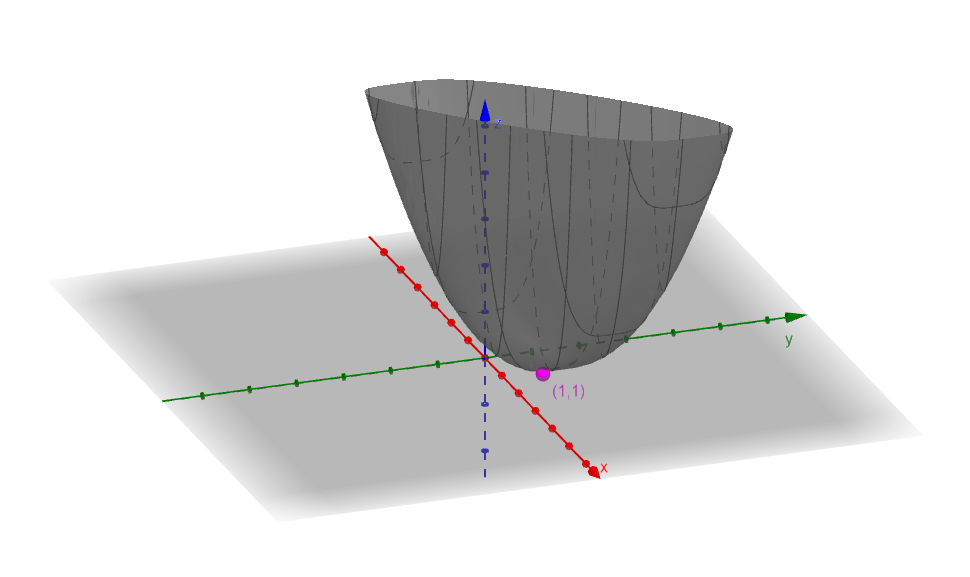
\includegraphics[width=0.5\textwidth]{Extremos20242c.png} % Cambia esta ruta por la ubicación de tu imagen
    \caption{Gráfica de $f$.}
    \label{fig:ejemplo} % Etiqueta para hacer referencia a la imagen
\end{figure}
\end{solution}
 no se pq no compila, desp lo arreglo -Vito
            
        \newpage
        \section{Fecha 11 de noviembre de 2024}
            %------------Ejercicio 1---------------------------------------

\begin{question}
    Sea la superficie $S = \{(x,y,z) \in \mathbb{R}^3 : x^2 + y^2 = z^2, 0 \leq z \leq 1\}$ y sea el campo $F(x,y,z) = (x + y^2 z, y + z^2 x^2, z)$. Hallar el flujo de $F$ a través de $S$ indicando la orientación elegida.
\end{question}

%------------Ejercicio 2---------------------------------------

\begin{question}
   Sea la superficie $S = \{(x,y,z) \in \mathbb{R}^3 : z + (y - 1)^2 + x^2 = 3, z \geq 0\}$ y sea $C \subset \mathbb{R}^3$ la curva dada por las ecuaciones
\[
C = \begin{cases} 
    y^2 - 2y - z + 1 = 0, \\
    y - x = 1.
\end{cases}
\]
Hallar el plano tangente a $S$ en $P$ para cada punto $P \in (S \cap C)$.
\end{question}

%------------Ejercicio 3---------------------------------------

\begin{question}
    Para la curva simple, cerrada y orientada $C$ formada por los segmentos de $(0,0)$ a $(1,1)$, de $(1,1)$ a $(0,1)$ y de $(0,1)$ vuelta al $(0,0)$, calcular
\[
\oint_C xy \, dx + \sqrt{y^2+1} \, dy.
\]
\end{question}

%------------Ejercicio 4---------------------------------------

\begin{question}
    Sea $\Omega = \{(x,y,z) \in \mathbb{R}^3 : 16x^2 + 4y^2 + z^2 \leq 1\}$ y sea $f$ una función continua sobre el intervalo $[0,1]$. Probar
\[
\iiint_\Omega f(\sqrt{16x^2 + 4y^2 + z^2}) \, dV = \frac{\pi}{2} \int_0^1 x^2f(x) \, dx.
\]

\textit{Nota: recordar que al multiplicar todos los elementos de una fila de una matriz por un número, el determinante de la matriz resultante es igual al de la original multiplicado por ese mismo número.}
\end{question}

%------------Solucion 1---------------------------------------
\newpage
\begin{solution} 
En primer lugar, se grafica la superficie a analizar:


   \begin{center}
        \begin{tikzpicture}
            \begin{axis}[
                    view={60}{20},
                    xlabel=$x$,
                    ylabel=$y$,
                    zlabel=$z$,
                    xmin=-1,
                    ymin=-1,
                    zmin=0,
                    xmax=1,
                    ymax=1,
                    zmax=2,
                    samples=50,
                    width=10cm,
                    height=12cm,
                    colormap/viridis,
                ]
                \addplot3[
            surf,
            domain=0:1,
            y domain=0:360,
            samples=30,
            samples y=60
        ]
        ({x*cos(y)},{x*sin(y)},{x}); % Parámetrico: x = r cos(θ), y = r sin(θ), z = r
            \end{axis}
        \end{tikzpicture}
    \end{center}

  

    La idea, es analizar la posibilidad de utilizar el teorema de Gauss. Podemos ver que $S$ no es una superficie cerrada.   Para ello, consideremos una superficie $S'$  cerrada tal  que $S \subseteq S'.$  Definamos   $S'=S\;\cup\;S_{tapa}\;$,  donde $S_1$, es la ``tapa'' superior que le "falta" al cono ``cortado''.  Algebraicamente $S_{tapa}=\{(x,y,z)\in \Re^{3} : x^2+y^2\le 1\;\land z=1\}$.

    Denotemos por $\Omega$  al cuerpo encerrado por $S'$. Al orientar $S'$ de manera exterior estamos en condiciones de usar el teorema de Gauss.
   \[
        \oiint _{S'} \mathbf{F}\cdot d\mathbf{A} =
        \iint _{S} \mathbf{F}\cdot d\mathbf{A} +
        \iint _{S_{tapa}} \mathbf{F}\cdot d\mathbf{A} +
        =\iiint _\Omega \grad \cdot \mathbf{F}\;dV \newline
     \]
    \[ 
        \iff \iint _{S} \mathbf{F}\cdot d\mathbf{A} =
        \iiint _\Omega \grad \cdot \mathbf{F}\;dV -
        \iint _{S_{tapa}} \mathbf{F}\cdot d\mathbf{A} 
    \]
   

    Resolvemos el primer t\'ermino.
    \begin{align*}
        \iiint _\Omega \grad \cdot \mathbf{F}\;dV = \iiint _\Omega3\:dV = 3\:\text{Vol}(\Omega)
    \end{align*}
    Pasando a  $\Omega$ en coordenadas cil\'indricas
    \[\begin{dcases}
            x=\rho \cos \phi \\
            y=\rho \sen \phi \\
            z=z
        \end{dcases}\] donde, $$0\leq\rho\leq z\:\land\:0\leq\phi\leq 2\pi \land 0\leq z \leq 1.$$

    Entonces nos queda    \[
        \text{Vol}(\Omega) =  \int_0^1  \int_0^{2\pi} \int_0^z  \rho\:d\rho\:d\phi \:dz=2\pi  \int_0^1\Big( \frac{\rho^2}{2}\Big|_0^z \Big) \:dz =  \pi   \int_0^1   z^2  \:dz= \frac{ \pi}{3}.
    \] Por lo cuál, 
     \begin{align*}
        \iiint _\Omega \grad \cdot \mathbf{F}\;dV =\pi
    \end{align*}

    Para clacular el segundo término, debemos parametrizar $S_{tapa}$.  Sea  $D_{\text{tapa}} = \{ (\rho, \phi) \in \mathbb{R}^2 : 0 \leq \rho \leq 1, \, 0 \leq \phi < 2\pi \}$ y  sea  $$\boldsymbol{\Sigma}:D_{tapa}\subset\Re^2\to\Re^3  \mbox{ tal que }   \boldsymbol{\Sigma}(\rho,\phi)=(\rho\cos(\phi),\rho\sin(\phi),1).$$
    Entonces podemos reescribir
    \[
        \iint _{S_{tapa}} \mathbf{F}\cdot d\mathbf{A}=\iint _{D_{tapa}} (\mathbf{F}\circ\boldsymbol{\Sigma})\cdot
        (\boldsymbol{\Sigma}_{\rho}\times\boldsymbol{\Sigma}_{\phi})\:d\mathbf{A}.
    \]
    Primero calculamos las derivadas parciales de la parametrizaci\'on.
    \begin{align*}
        \boldsymbol{\Sigma}_{\rho} & =(\cos(\phi),\sin(\phi),0) \\
        \boldsymbol{\Sigma}_{\phi} & =(-\rho \sin(\phi),\rho \cos(\phi),0)
    \end{align*}
    Entonces
    \[
        \boldsymbol{\Sigma}_{\rho}\times\boldsymbol{\Sigma}_{\phi}=(0,0,r)=\boldsymbol{\eta}.
    \]
    Podemos observar que $\boldsymbol{\eta}$ preserva la orientaci\'on  para $S_{tapa}$ heredada  por la orientaci\'on exterior de $S'$ elegida anteriormente para poder aplicar el teorema de Gauss, ya que $r\geq0$. En otras palabras,  $\boldsymbol{\eta}$ ``apunta''  hacia el exterior de $\Omega$.  
   
    Calculamos el término, 
    \[
         \iint _{D_{tapa}} (\mathbf{F}\circ\boldsymbol{\Sigma})\cdot
        (\boldsymbol{\Sigma}_{\rho}\times\boldsymbol{\Sigma}_{\phi})\:d\mathbf{A}=\int_0^1  \int_0^{2\pi}   \rho\:d\rho\:d\phi =2\pi  \Big( \frac{\rho^2}{2}\Big|_0^1 \Big) \:dz =  \pi   
    \]

    $$\therefore\;\iint _{S} \mathbf{F}\cdot d\mathbf{A}=\pi - \pi=0$$
\end{solution}

%------------Solucion 2---------------------------------------

\begin{solution}
En primer lugar, vamos a encontrar los puntos $P$ donde la superficie $S$ intersecta la curva $C$. Escribiremos las ecuaciones que definen a la curva $C $ en terminos de $y$:
   \[
   \begin{cases}
   y^2 - 2y - z + 1 = 0 \\
   y - x = 1
   \end{cases}
   \iff
   \begin{cases}
    z= y^2 - 2y  + 1 \\
    x =y- 1
   \end{cases}
  \]
Sustituyendo estos valores de y en las ecuaciones paramétricas de la curva, obtenemos los puntos de intersección
 \[
    (y^2 - 2y + 1) + (y - 1)^2 + (y - 1)^2 = 3
 \]
Expandiendo los términos y factorizando llegamos a que
 \[
    3y(y - 2) = 0 \iff 
    \begin{cases}
    y=0\\
    y=2
    \end{cases}
 \]

Ahora simplemente reemplazamos en las ecuaciones de la curva para obtener los valores de $x$ y $z$, con lo cual determinamos dos puntos:
\[
    P_1=(-1,0,1)
 \]
\[
    P_2=(1,2,1)
 \]
\end{solution}
Ahora que obtuvimos los puntos, vamos a buscar cada plano tangente a la superificie $S$ en los puntos $P_1 $ y $ P_2$. Recordamos la formula de plano tangente a una superficie: $\pi: \grad f(xo,yo,zo).(x-xo,y-yo,z-zo)=0$, donde definimos $f$ como $f(x,y,z)=z + (y - 1)^2 + x^2-3$ y calculamos su gradiente
\[
   \grad f(xo,yo,zo)=(2x,2(y-1),1)\quad\backslash 
   \begin{cases}
   \grad f(-1,0,1)=(-2,-2,1)\\
   \grad f(1,2,1)=(2,2,1)
   \end{cases}
 \]
 Por último, calculamos los planos tangentes en cada punto
 \[
 \pi_1: (-2,-2,1)(x+1,y,z-1)=0 \iff -2x-2-2y+z-1=0\iff -2x-2y+z-3=0
 \]
 \[
 \pi_2: (2,2,1)(x-1,y-2,z-1)=0 \iff 2x-2+2y-4+z-1=0\iff 2x+2y+z-7=0
 \]
\newline
$\therefore\;$ Los planos tangentes a $S$ en $P$ para cada punto $P \in (S \cap C)$ son:
\[
\pi_1:-2x-2y+z=3\quad \text {para  }  P_1=(-1,0,1)
 \]
 \[
 \pi_2:2x+2y+z=7\quad \text {para  }  P_2=(1,2,1)
 \]


%------------Solucion 3---------------------------------------

\begin{solution}
    Empezamos gráficando la curva a analizar, la cual se recorre en sentido antihorario
   \begin{center}
    \begin{tikzpicture}[scale=3]
        % Ejes coordenados
        \draw[->] (-0.2,0) -- (1.2,0) node[right] {\footnotesize $x$};
        \draw[->] (0,-0.2) -- (0,1.2) node[above] {\footnotesize $y$};

        % Puntos
        \filldraw (0,0) circle (1pt) node[below left] {\footnotesize (0,0)};
        \filldraw (1,1) circle (1pt) node[above right] {\footnotesize (1,1)};
        \filldraw (0,1) circle (1pt) node[above left] {\footnotesize (0,1)};
        
        % Lados del triángulo
        \draw[thick] (0,0) -- (1,1) -- (0,1) -- cycle;
    \end{tikzpicture}
\end{center}
    Se nos solicita calcular la circulación del campo vectorial $F$ a lo largo de la curva cerrada $C$, siendo $F(x,y)=(xy,\sqrt{y^2+1)}$
    \[
\oint_C xy \, dx + \sqrt{y^2+1} \, dy = \oint_C(xy,\sqrt{y^2+1)}dxdy
\]
Como hablamos de una curva cerrada, simple y orientada en sentido antihorario, utilizamos el teorema de Green. En el mismo, la región $D$ encerrada la definimos como $D = \{ (x, y) \in \mathbb{R}^2 : 0 \leq y \leq 1, \, 0 \leq x < y \}$ la cuál graficamos para comprenderla mejor:
  \begin{center}
        \begin{tikzpicture}
            \begin{axis}[
                    axis lines=center,
                    axis equal,
                    xlabel=$x$,
                    ylabel=$y$,
                    xmin=0,
                    xmax=1,
                    ymin=0,
                    ymax=1.2,
                    xtick distance=1,
                    ytick distance=1,
                ]
                \addplot[name path=A, draw=none]{x} node[pos=0.55, right]{$y=x$};
                \addplot[name path=B, draw=none]{1};
                \addplot[fill=violet!90, opacity=0.7]fill between[of=A and B, soft clip={domain=0:1}];
            \end{axis}
        \end{tikzpicture}
    \end{center}

Por lo tanto, tenemos que 
\[
 \oint_C(xy,\sqrt{y^2+1)}dxdy=\iint _D \mathbf{rot(F)}\cdot d\mathbf{A}=\iint _D 0-x\cdot d\mathbf{A}=-\iint _D x\cdot d\mathbf{A}
\]
Utilizando los extremos de integración de la region $D$, resolvemos
 \[
         -\iint _D x\cdot d\mathbf{A}=-\int_0^1  \int_0^{y}   x\:dx\:dy =-  \int_0^1\Big( \frac{x^2}{2}\Big|_0^y \Big) \:dy=-\Big( \frac{y^3}{6}\Big|_0^1 \Big)=-\frac{1}{6}
    \]
$$\therefore\;\oint_C xy \, dx + \sqrt{y^2+1} \, dy =-\frac{1}{6}$$


\end{solution}

%------------Solucion 4---------------------------------------

\begin{solution}
 En primer lugar, podemos identificar que $\Omega $  es una elipsoide, por lo cuál vamos a comenzar realizando una transformación de la misma a coordenadas esfericas

\[
T(x,y,z) = \left( \frac{1}{4} \rho \cos(\theta)\sin( \varphi), \frac{1}{2} \rho \sin(\theta)\sin( \varphi),  \rho \cos(\varphi) \right)
\]
Donde $\Omega^*$ es el dominio transformado en coordenadas esféricas, definido por
 \[\Omega^*=\begin{cases}
            \;\rho \in [0,1] \\[5pt]
            \; \varphi \in [0,\pi] \\[5pt]
            \;\theta \in [0,2\pi]
        \end{cases}
    \]
De esta manera $T:\Omega^* \rightarrow \Omega$ es una transformación, cuyo determinante de la matriz Jacobiana se puede calcular utilizando el conocido de esfericas y la ayuda de la nota:

\[
J_T(\rho, \theta,\varphi) = \left| \det D_T (\rho, \theta,\varphi) \right| = \frac{1}{4}\frac{1}{2}\rho^2\sin(\varphi)
\]
Para empezar a demostrar la igualdad, partiremos del término izquierdo, donde definiremos una función $g:\Re^3\rightarrow\Re, g(x,y,z)=f(\sqrt{16x^2 + 4y^2 + z^2})$

\[
\iiint_\Omega f(\sqrt{16x^2 + 4y^2 + z^2}) \, dV=\iiint_{\Omega^*}g \circ T (\rho, \theta,\varphi).J_T(\rho, \theta,\varphi)dV=\iiint_{\Omega^*}f(\rho) \frac{1}{8}\rho^2\sin(\varphi)dV
\]
Resolviendo la integral,
\[
\frac{1}{8}\iiint_{\Omega^*}f(\rho) \rho^2\sin(\varphi)dV=\frac{1}{8}\int_0^{1} f(\rho) \rho^2d\rho.\int_0^{2\pi}d\theta.\int_0^{\pi}\sin(\varphi)d\varphi= \frac{\pi}{2}\int_0^{1} f(\rho) \rho^2d\rho
\]

$$\therefore\;\iiint_\Omega f(\sqrt{16x^2 + 4y^2 + z^2}) \, dV = \frac{\pi}{2}\int_0^{1} f(\rho) \rho^2d\rho$$

\end{solution}

            
        \newpage
        \section{Fecha recuperatorio extra}
            %------------------Ejercicio 1--------------------------------

\begin{question}
    Sean  $V=\{ (x,y,z) \in \mathbb{R}^{3}:  x\leq 0, \;  y
        \leq 0, \;  0 \leq  z \leq 1-x^{2}-y^{2}  \}$ y
    $S=\{ (x,y,z) \in \mathbb{R}^{3}:  x\geq 0, \; y \geq 0,
        z\geq 0,\;  z = 1-x^{2}-y^{2}  \}$.
    Calcluar el volumen de $V$ y el \'area de $S$.
\end{question}

%------------------Ejercicio 2--------------------------------

\begin{question}
    Sean  $S$ una superficie  esf\'erica de radio $R$ con
    centro en el primer octante  y  $\mathbf{F}$ un campo de
    clase $C^{1}$  con $\grad\cdot\mathbf{F}(x,y,z) = x+y+z$.
    Probar que  el flujo saliente de $\mathbf{F}$ a trav\'es de
    $S$  es no negativo.
\end{question}

%------------------Ejercicio 3--------------------------------

\begin{question}
    Sean  $C$ el borde del tri\'angulo de v\'ertices $(-1,0)$,
    $(1,0)$ y $(0,1)$ y el campo $\mathbf{F}(x,y) =
        \Big(e^{\cos(x)+x^{2}}+xy^{2}+2y, \ln(1+e^{y^{2}}) +yx^{2}+3x \Big).$
    Calcular,  indicando la orientaci\'on elegida:
    $$ \int_{C} \mathbf{F}\cdot ds$$
\end{question}

%------------------Ejercicio 4--------------------------------

\begin{question}
    Probar que el campo $\mathbf{F}(x,y) = \Big(y e^{xy}+y\cos(xy)
        ,xe^{xy}+\cos(xy) x \Big)$ es conservativo.  Dada $C$ la curva
    parametrizada por $\boldsymbol{\alpha}(t) = (t^{2},t)$ con $t
        \in [0,1]$ calcular el trabajo realizado por $\mathbf{F}$ sobre $C.$
\end{question}

\newpage

%------------------Solucion 1--------------------------------

\begin{solution}
    Nos piden calcular $\iiint_V dV$ y $\iint_S dA$. Para la
    integral de volumen conviene trabajar en coordenadas
    cil\'indricas y para la de superficie habr\'a que parametrizar.

    \begin{center}
        \begin{tikzpicture}
          \begin{axis}[
                axis lines=center,
                axis equal,
                view={110}{20},
                xlabel=$x$,
                ylabel=$y$,
                zlabel=$z$,
                xtick={1},
                ytick={-1,1},
                ztick={1,1.5},
                xmin=-1,
                ymin=-0.5,
                zmin=0,
                xmax=1.7,
                ymax=1.1,
                zmax=1,
                samples=30,
                width=14cm,
                height=12cm,
                colormap/viridis,
                xlabel style={at={(0.31,0.2)}},
            ]
            \addplot3 [surf, opacity=0.8, draw=none, restrict z to domain=0:1,
            data cs=polar, domain=0:90, y domain=0:1] (x, y, 1-y^2);
          \end{axis}
        \end{tikzpicture}
      \end{center}

    Aplicando la transformaci\'on $V \rightarrow V^*$ queda
    \begin{align*}
        V^*      & =\{(\rho, \phi, z)\in\Rn{3}: \rho\cos\phi \leq 0,\;
        \rho\sen\phi \leq 0,\; 0 \leq z \leq 1-\rho^2\}               \\
        \iff V^* & =\{(\rho, \phi, z)\in\Rn{3}: \pi \leq \phi \leq
        \frac{3}{2}\pi,\; 0 \leq z \leq 1,\; 0 \leq \rho \leq
        \sqrt{1-z} \}.
    \end{align*}
    Y por el teorema de cambio de variable tenemos que
    \begin{align*}
        \iiint_V dV & = \iiint_{V^*} \rho\:dV = \int_\pi^{\frac{3}{2}\pi}
        \int_0^1\int_0^{\sqrt{1-z}}\rho\:d\rho dz d\phi                   \\
                    & =\frac{\pi}{2}\int_0^1\frac{1}{2}(1-z)\:dz =
        \frac{\pi}{8}.
    \end{align*}

    Para parametrizar $S$, llamamos
    \[
        D = \{(\rho, \phi)\in\Rn{2} : \pi\leq\phi\leq\frac{3}{2}\pi,\;
        0\leq\rho\leq 1\}.
    \]
    y
    \[
        \boldsymbol{\Sigma}:D\subset\Rn{2}\rightarrow\Rn{3}\text{ tal que }
        \boldsymbol{\Sigma}(\rho,\phi)=(\rho\cos\phi,\;\rho\sen\phi,\;\rho^2).
    \]
    Calculamos las derivadas paraciales de $\boldsymbol{\Sigma}$.
    \begin{align*}
        \boldsymbol{\Sigma}_{\rho}&=(\cos \phi,\;\sen \phi,\; 2\rho)\\
        \boldsymbol{\Sigma}_\phi&=(  -\rho \sen \phi,\;\rho \cos \phi,\;0)
        \end{align*}
    Luego
    $$
        \boldsymbol{\Sigma}_{\rho} \times\boldsymbol{\Sigma}_\phi =
        (-2\rho^2 \cos\phi  , \;-2\rho^2 \sen \phi, \;\rho),
    $$ 
    $$\|\boldsymbol{\Sigma}_{\rho} \times\boldsymbol{\Sigma}_\phi\|
        = \rho\sqrt{4\rho^2+1}.
    $$ 
    Entonces escribimos, por definici\'on, el \'area de $S$ como
    \[
        \iint_S dA = \iint_D \| \boldsymbol{\Sigma}_{\rho}
        \times\boldsymbol{\Sigma}_\phi\|\:d\rho d\phi = \int_\pi^{\frac{3}{2}\pi}\int_0^1\rho\sqrt{4\rho^2+1}\:d\rho d\phi.
    \]
    Nos queda la misma integral que \eqref{eq:integral1}, s\'olo que con distintos l\'imites de integraci\'on. Por lo que, procediendo de la misma manera, sustituyendo $u = 4\rho^2+1$, obtenemos
    \begin{gather*}
        \iint_S dA =
        \frac{1}{8}\int_\pi^{\frac{3}{2}\pi}\int_1^5\sqrt{u}\:du =
        \frac{\pi}{16}\frac{u^{\frac{3}{2}}}{\frac{3}{2}}\Bigg\lvert_1^5 =
        \frac{\pi}{24}(\sqrt{125}-1).
    \end{gather*}
\end{solution}

%------------------Solucion 2--------------------------------

\begin{solution}
    Tenemos que $S=\{(x,y,z)\in\Rn{3}:
        (x-x_0)^2+(y-y_0)^2+(z-z_0)^2=R^2\}$, con $R>0$ y
    $(x_0,y_0,z_0)$ en el primer octante.
    Por el teorema de la divergencia
    \begin{equation}
        \iint_S \mathbf{F}\cdot\:d\mathbf{A} = \iiint_\Omega
        \grad\cdot\mathbf{F}\:dV
        = \iiint_\Omega (x+y+z)\:dxdydz, \label{eq: divEj2}
    \end{equation}
    tomando la orientaci\'on de $S$ como exterior.

    Aplicando una tranformaci\'on a coordenadas esf\'ericas, tal que
    \begin{align*}
        x & =\rho\sen\phi\cos\theta+x_0 \\
        y & =\rho\sen\phi\sen\theta+y_0 \\
        z & =\rho\cos\phi+z_0,
    \end{align*}
    nos queda el conjunto $S^*$
    \[
        S^*=\{(\rho,\phi,\theta)\in\Rn{3}:0\leq\rho\leq R,\;
        0\leq\theta\leq2\pi,\;0\leq\phi\leq\pi\}.
    \]
    De la ecuaci\'on \eqref{eq: divEj2} y usando el teorema
    de cambio de variable,
    \begin{gather*}
        \iiint_\Omega (x+y+z) \:dV = \iiint_{\Omega^*}
        (\rho\sen\phi\cos\theta + \rho\sen\phi\sen\theta
        + \rho\cos\phi + x_0 + y_0 + z_0)
        \:\rho^2\sen\phi\:d\rho d\theta d\phi=\\
        = \int_0^\pi\int_0^{2\pi}\int_0^R (\rho\sen\phi\cos\theta
        + \rho\sen\phi\sen\theta + \rho\cos\phi
        + x_0 + y_0 + z_0)\rho^2\sen\phi\:d\rho d\theta d\phi.
    \end{gather*}
    Al distribuir el $\rho^2\sen\phi$ entre los primeros dos
    t\'erminos, queda para estos \(\rho^3\sen\phi^2\cos\theta\) y \\
    \(\rho^3\sen\phi^2\sen\theta\); que al integrarlos entre 0
    y $2\pi$, con respecto a $\theta$, se anulan. Entonces queda,
    distribuyendo la suma del integrando,
    \[
        \int_0^\pi\int_0^{2\pi}\int_0^R \rho^3\cos\phi\sen\phi\:
        d\rho d\theta d\phi + \int_0^\pi\int_0^{2\pi}\int_0^R
        (x_0 + y_0 + z_0)\rho^2\sen\phi\:d\rho d\theta d\phi.
    \]
    A su vez, la primer integral es 0 porque al integrar una
    funci\'on peri\'odica impar, $\cos\phi\sen\phi$, en un
    semi per\'iodo \'esta se anula. Por \'ultimo queda
    \[
        (x_0 + y_0 + z_0)\int_0^\pi\int_0^{2\pi}\int_0^R
        \rho^2\sen\phi\:d\rho d\theta d\phi = (x_0 + y_0 + z_0)
        \frac{4}{3}\pi R^3 > 0,
    \]
    pues $(x_0, y_0, z_0)$ pertenece al primer octante.
    Por lo que queda demostrado que el flujo es positivo.

    \textcolor{red}{por qu\'e ser\'ia -no negativo-? por ej. 
    cuando R = 0 o cuando el centro de la esfera es el origen es = 0}
\end{solution}

%------------------Solucion 3--------------------------------

\begin{solution}
    Nos piden integrar sobre la siguiente curva $C$.

    \begin{center}
        \begin{tikzpicture}
            \begin{axis}[
                    axis lines=center,
                    axis equal,
                    xlabel=$x$, ylabel=$y$,
                    xmin=-1.5, xmax=1.5,
                    ymin=0, ymax=1,
                    xtick distance=1, ytick distance=1,
                ]
                \draw[cyan, thick] (-1,0) -- (1,0) -- (0,1) -- cycle;
            \end{axis}
        \end{tikzpicture}
    \end{center}

    Tomamos la orientaci\'on de $C$ como antihoraria.
    % depende de como este definido el interior de una curva
    Dado que el tri\'angulo $T$  es simplemente conexo,   $T
        \in \text{dom}(\mathbf{F})$ y $\mathbf{F}\in \mathcal{C}^1$, entonces
    por el teorema de Green
    \[
        \oint_C \mathbf{F}\cdot d\mathbf{s} = \iint_T
        \grad\times\mathbf{F}\:dA.
    \]
    Como $\grad\times\mathbf{F} = 1$, queda que \[\oint_C
        \mathbf{F}\cdot d\mathbf{s} = \iint_T dA = \textcolor{red}{Area}(T)
        = \frac{2\cdot1}{2} = 1.\]
\end{solution}

%------------------Solucion 4--------------------------------

\begin{solution}
    Ya que nos piden demostrar que $\mathbf{F}$ es conservativo
    y calcular una integral de l\'inea sobre una curva no
    cerrada nos conviene buscar, si es que existe, la funci\'on
    potencial de $\mathbf{F}$. Nos encontramos con la ecuaci\'on
    $\grad f = \mathbf{F}$, la cual describe el siguiente
    sistema de ecuaciones diferenciales.
    \[
        \begin{dcases}
            f_x(x,y) = ye^{xy} + y \cos{(xy)} \\[.2cm]
            f_y(x,y) = xe^{xy} + x \cos{(xy)}
        \end{dcases}
    \]
    Mirando cada t\'ermino detenidamente se puede llegar a
    la conclusi\'on de que $$f(x,y) = e^{xy} + \sen{(xy)} + C,
        \mbox{ con } C\in\R$$ es soluci\'on del sistema. Lo que
    significa que $\mathbf{F}$ es un campo conservativo.

    Luego para calcular $\int_C \mathbf{F}\cdot d\mathbf{s}$
    utilizamos el siguiente teorema.
    \[
        \int_C \grad f\cdot d\mathbf{s} =
        f(\boldsymbol{\alpha}(1)) - f(\boldsymbol{\alpha}(0)) =
        f((1,1)) - f((0,0)) = e + \sen1 - 1.
    \]
\end{solution}



    
\end{document}
